% =====================================================================================
%  Solving Poker: the numerical analysis behind poker solvers
%  Numerical Analysis Research Club -- ~60 minutes
%  Compile slides:  pdflatex talk.tex   (twice)
%  Compile notes :  pdflatex -jobname=talk-notes "\def\notesmode{1}% =====================================================================================
%  Solving Poker: the numerical analysis behind poker solvers
%  Numerical Analysis Research Club -- ~60 minutes
%  Compile slides:  pdflatex talk.tex   (twice)
%  Compile notes :  pdflatex -jobname=talk-notes "\def\notesmode{1}% =====================================================================================
%  Solving Poker: the numerical analysis behind poker solvers
%  Numerical Analysis Research Club -- ~60 minutes
%  Compile slides:  pdflatex talk.tex   (twice)
%  Compile notes :  pdflatex -jobname=talk-notes "\def\notesmode{1}% =====================================================================================
%  Solving Poker: the numerical analysis behind poker solvers
%  Numerical Analysis Research Club -- ~60 minutes
%  Compile slides:  pdflatex talk.tex   (twice)
%  Compile notes :  pdflatex -jobname=talk-notes "\def\notesmode{1}\input{talk.tex}"
%  This is the simplified deck that goes with the live demonstration (../app). The longer version is talk-detailed.tex.
%  Every number marked "we computed" comes from ../solver (see numbers.tex, generated by gen_numbers.py)
% =====================================================================================
\providecommand\notesmode{0}
\ifnum\notesmode=1 \PassOptionsToClass{handout}{beamer}\fi
\documentclass[10pt,aspectratio=169]{beamer}
\usetheme[progressbar=frametitle,numbering=fraction,block=fill]{metropolis}
\ifnum\notesmode=1
  \setbeameroption{show only notes}
\fi
\usepackage[T1]{fontenc}
\usepackage{lmodern}
\usepackage{amsmath,amssymb,mathtools}
\usepackage{booktabs}
\usepackage{xcolor}
\usepackage{tikz}
\usetikzlibrary{arrows.meta,positioning,calc,shapes.geometric,fit,backgrounds,decorations.pathreplacing}
\usepackage{graphicx}
\usepackage{fancyvrb}
\graphicspath{{../figs/}}
\input{numbers.tex}

% ---------- palette (validated categorical slots + inks) ----------
\definecolor{cblue}{HTML}{2A78D6}
\definecolor{corange}{HTML}{EB6834}
\definecolor{caqua}{HTML}{1BAF7A}
\definecolor{cyellow}{HTML}{EDA100}
\definecolor{cmagenta}{HTML}{E87BA4}
\definecolor{ink}{HTML}{0B0B0B}
\definecolor{ink2}{HTML}{52514E}
\definecolor{paper}{HTML}{FCFCFB}
\definecolor{lightblue}{HTML}{CDE2FB}
\definecolor{lightgray}{HTML}{E4E3DF}
\definecolor{felt}{HTML}{1F6B4A}
\definecolor{suitred}{HTML}{C8102E}
\definecolor{suitblue}{HTML}{1C5CAB}
\definecolor{suitgreen}{HTML}{147A3A}
\setbeamercolor{normal text}{fg=ink,bg=paper}
\setbeamercolor{alerted text}{fg=corange}
\setbeamercolor{progress bar}{fg=cblue,bg=lightgray}
\setbeamercolor{frametitle}{bg=ink,fg=paper}
\setbeamercolor{block title}{bg=lightblue,fg=ink}
\setbeamercolor{block body}{bg=lightblue!35,fg=ink}
\setbeamercolor{example text}{fg=caqua!80!black}
\metroset{titleformat frame=regular}
\setbeamerfont{note page}{size=\scriptsize}

% ---------- notation ----------
\newcommand{\src}[1]{{\par\vfill\hfill\tiny\color{ink2}#1}}
\newcommand{\R}{\mathbb{R}}
\newcommand{\ex}{\operatorname{expl}}
\newcommand{\tagP}{\tikz[baseline=-0.6ex]\node[fill=felt,text=white,rounded corners=1.5pt,inner sep=1.6pt,font=\tiny\bfseries]{POKER};}
\newcommand{\tagM}{\tikz[baseline=-0.6ex]\node[fill=cblue,text=white,rounded corners=1.5pt,inner sep=1.6pt,font=\tiny\bfseries]{MATH};}
\newcommand{\tagO}{\tikz[baseline=-0.6ex]\node[fill=corange,text=white,rounded corners=1.5pt,inner sep=1.6pt,font=\tiny\bfseries]{NEW};}

% ---------- playing cards (four-colour deck) ----------
\colorlet{suit-s}{ink}\colorlet{suit-h}{suitred}\colorlet{suit-d}{suitblue}\colorlet{suit-c}{suitgreen}
\newcommand{\suitsym}[1]{\ensuremath{\csname suit@#1\endcsname}}
\makeatletter
\def\suit@s{\spadesuit}\def\suit@h{\heartsuit}\def\suit@d{\diamondsuit}\def\suit@c{\clubsuit}
\makeatother
\newcommand{\pcard}[3][1]{% [scale]{rank}{suit}
  \tikz[baseline=-0.7ex]{\node[draw=ink2,fill=white,rounded corners=2.5pt,minimum width=#1*0.62cm,
  minimum height=#1*0.86cm,inner sep=0pt,text=suit-#3,font=\bfseries\sffamily]
  {\shortstack{#2\\[-1pt]\suitsym{#3}}};}}
\newcommand{\cardback}{\tikz[baseline=-0.7ex]{\node[draw=white,fill=suitred!80!black,rounded corners=2pt,
  minimum width=0.42cm,minimum height=0.6cm,inner sep=0pt]{};}}

\title{Solving Poker}
\subtitle{The numerical analysis behind poker solvers\\ --- and a second-order finish for them}
\author{Numerical Analysis Research Club}
\date{}

\begin{document}

% =====================================================================================
\begin{frame}
  \titlepage
\note{
\textbf{Timing plan for 60 minutes.} Opening and rules 5 $\cdot$ Games, equilibria and the linear program 9 $\cdot$
Regret minimisation and CFR 9 $\cdot$ Live demonstration 12 $\cdot$ The new method 13 $\cdot$ Results, limits and wrap-up 8.
That leaves about four minutes for questions during the talk.\\[4pt]
If running late, shorten the demonstration to its five minute version (see \texttt{app/DEMO\_NOTES.md}) and give the slide
``Making it robust and fast'' one sentence.\\[4pt]
Opening line: ``Ten years ago the best poker players in the world lost to programs whose core is a few lines of
arithmetic repeated a few billion times. This talk is about that arithmetic, read as numerical analysis, and about
what a numerical analyst can add to it.''\\[4pt]
The slides alternate between \textsc{poker} (green tag) and \textsc{math} (blue tag). The orange tag \textsc{new} marks
our own contribution. Every number that we computed comes from the Python solver in the repository. The more detailed
version of this deck, with all citations and extra slides, is \texttt{talk-detailed.pdf}.
}
\end{frame}

% =====================================================================================
\begin{frame}{\tagP\ Ten years of superhuman poker}
\begin{columns}[T]
\column{0.58\textwidth}
In 2015 a program called Cepheus essentially solved two-player limit hold'em.

\medskip
In 2017 two programs, DeepStack and Libratus, beat professional players at the no-limit game, which is far larger.
In 2019 Pluribus did the same at a table of six.

\medskip
Today every serious player studies with a \alert{solver}. You describe one situation, and the program computes how
to play every possible hand in it.

\medskip
All of these programs share one simple iteration. This talk explains it and then tries to improve on it.
\column{0.4\textwidth}
\centering
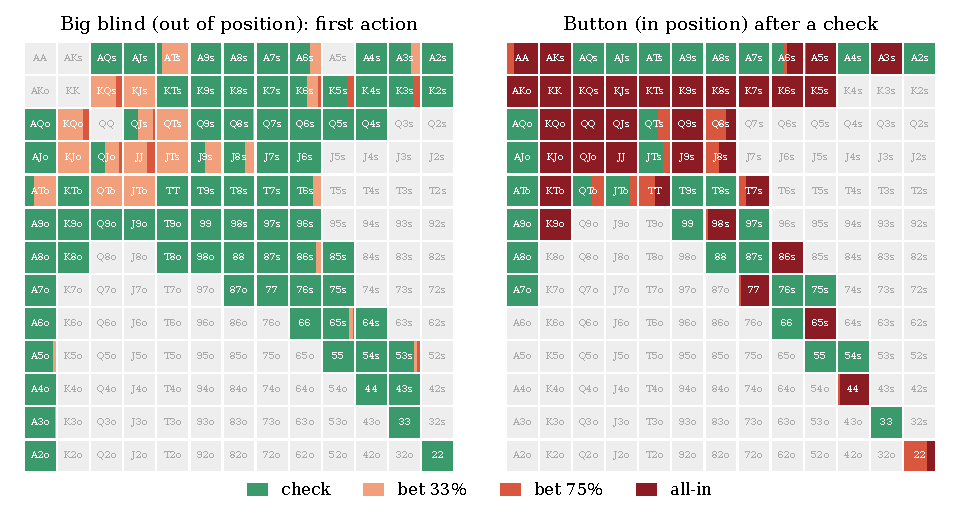
\includegraphics[height=0.6\textheight,trim=0 22 245 0,clip]{grid_root.pdf}\\[-2pt]
{\scriptsize\color{ink2} A solver's answer, computed by our own code. Each square is a starting hand and the colours are actions.}
\end{columns}
\note{
The common core of all these programs is an iterative method, counterfactual regret minimisation, applied to a very large
saddle-point problem. Libratus and DeepStack add abstraction (shrinking the game) and subgame solving
(solving again the part of the game you are actually in), but the inner loop is still a method of the CFR family.\\[3pt]
Commercial solvers such as PioSolver, GTO+ and GTO Wizard are what human players use. You give the board, the
two ranges and the allowed bet sizes, and the program computes an equilibrium of that subgame. The picture on the right is
exactly such an output, produced by our solver for the river situation that we use for the whole talk.\\[3pt]
References if asked: Bowling et al., Science 2015. Morav\v{c}\'ik et al., Science 2017. Brown and Sandholm, Science 2018 and 2019.
}
\end{frame}

% =====================================================================================
\begin{frame}{The plan: poker $\leftrightarrow$ math}
\centering
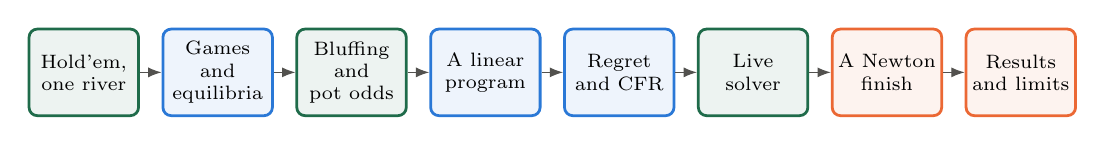
\begin{tikzpicture}[x=1cm,y=1cm,every node/.style={font=\scriptsize}]
  \foreach \i/\t/\c in {0/{Hold'em,\\ one river}/felt, 1/{Games and\\ equilibria}/cblue, 2/{Bluffing and\\ pot odds}/felt,
                       3/{A linear\\ program}/cblue, 4/{Regret\\ and CFR}/cblue, 5/{Live\\ solver}/felt,
                       6/{A Newton\\ finish}/corange, 7/{Results\\ and limits}/corange}{
    \node[draw=\c,line width=1pt,rounded corners=3pt,text width=1.25cm,minimum height=1.1cm,align=center,
          inner sep=2pt,fill=\c!8] (n\i) at (1.7*\i,0) {\t};
  }
  \foreach \i [evaluate=\i as \j using int(\i+1)] in {0,...,6} { \draw[-{Latex},ink2] (n\i) -- (n\j); }
\end{tikzpicture}

\vspace{1.4em}
\raggedright
The equilibrium of a poker game is the solution of a very large and very structured saddle-point problem.
Solvers attack it with a first-order method whose steps are cheap and whose last digits are slow.

\medskip
In the middle of the talk we solve a real hand live in the browser and look at the answer together.

\medskip
Our own contribution comes last. We treat the end of the solve as a nonsmooth equation and finish it with a Newton
method, which reaches machine precision where the first-order method would need millions of iterations.
\note{
Say what the audience will get. First, enough poker to read the output of a solver. Second, the mathematics of why CFR converges
and why it is fast in practice. Third, a live demonstration in which they can ask for any change to the hand. Fourth, a new method
from the numerical optimisation toolbox, with honest results: where it wins by orders of magnitude, and where it does not yet.
}
\end{frame}

% =====================================================================================
\begin{frame}{\tagP\ Texas hold'em in one slide}
\begin{columns}[T]
\column{0.5\textwidth}
Each of the two players is dealt two private cards. Five public cards, the \emph{board}, are then revealed in three
stages called the flop, the turn and the river.

\medskip
There is a round of betting before the flop and after each stage. A player may check, bet, call, raise or fold, and in the
no-limit game a bet can be any size up to the player's stack.

\medskip
If nobody folds, the best five-card hand made from the seven available cards wins the pot.
\column{0.48\textwidth}
\centering
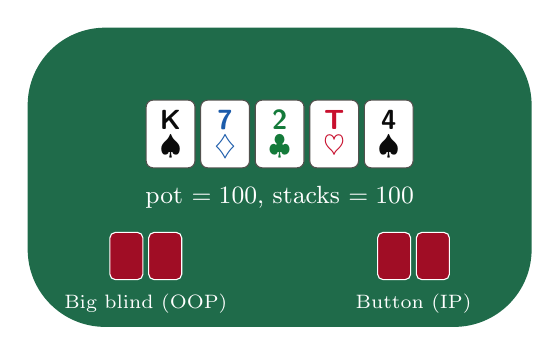
\begin{tikzpicture}
  \fill[felt,rounded corners=28pt] (-3.2,-1.9) rectangle (3.2,1.9);
  \node at (0,0.55) {\pcard{K}{s}\,\pcard{7}{d}\,\pcard{2}{c}\,\pcard{T}{h}\,\pcard{4}{s}};
  \node[text=white,font=\small] at (0,-0.25) {pot $= 100$, stacks $= 100$};
  \node at (-1.7,-1.0) {\cardback\,\cardback};
  \node at (1.7,-1.0) {\cardback\,\cardback};
  \node[text=white,font=\scriptsize] at (-1.7,-1.6) {Big blind (OOP)};
  \node[text=white,font=\scriptsize] at (1.7,-1.6) {Button (IP)};
\end{tikzpicture}\\[4pt]
{\small Our running example is the \alert{river}, the last round of betting.\\
The big blind acts first, which is called being out of position.}
\end{columns}
\note{
Keep this light, since most of the audience has played or watched poker. The key structural fact is that the board is
public and the two hole cards are private. A strategy must therefore be a function of
the public history and your own cards. You do not know the opponent's cards, only a probability distribution over them,
which poker players call a \textbf{range}.\\[3pt]
The river situation is fixed for the whole talk: board K$\spadesuit$ 7$\diamondsuit$ 2$\clubsuit$ T$\heartsuit$ 4$\spadesuit$, pot 100, both players
have 100 behind. The big blind may check or bet 33\% or 75\% of the pot or go all-in. Facing a bet you may fold, call or go all-in.
The live demonstration uses exactly this table.
}
\end{frame}

% =====================================================================================
\begin{frame}{\tagP\ Ranges: what a solver takes as input}
\begin{columns}[T]
\column{0.6\textwidth}
\centering
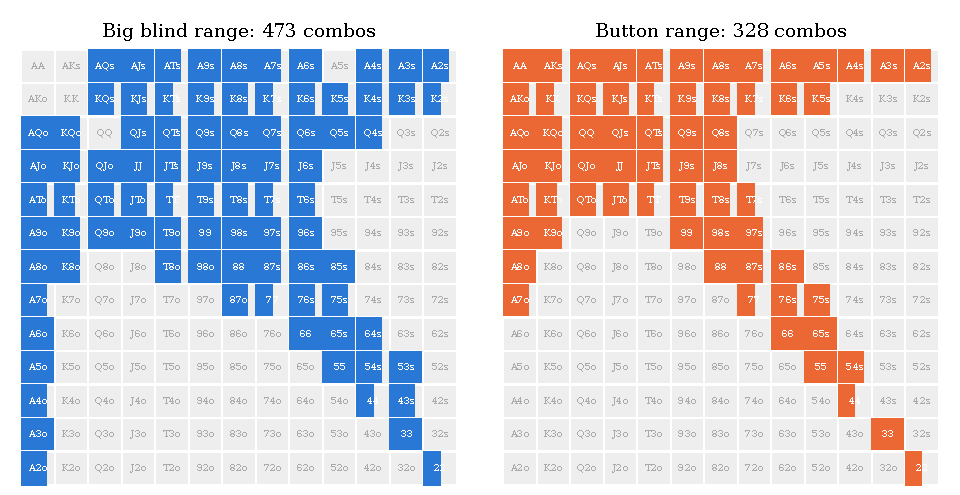
\includegraphics[width=\linewidth]{ranges.pdf}
\column{0.38\textwidth}
A \textbf{range} is a probability vector over the two-card hands a player can hold. There are 1326 such hands, and 1081
once the five board cards are known.

\medskip
In our example the big blind called a raise before the flop and the button made that raise, so the two ranges are
different.

\medskip
The solver returns, for every point of the betting and for every hand, a probability for each action.
\end{columns}
\note{
The 13 by 13 grid is the standard poker picture. Pairs are on the diagonal, suited hands above it and offsuit hands below it.
Each cell is a class of hands, for example AKs stands for 4 combinations. Mathematically the input is two nonnegative vectors
$r_1\in\R^{n_1}$ and $r_2\in\R^{n_2}$. Two hands that share a card cannot both be dealt, which is called card removal, and it is a 0/1
compatibility matrix $C$ between the ranges. Both will appear in the formulas later.\\[3pt]
The width of each bar shows how many combinations are still possible given the board. The king of spades is on the board, so there
are fewer hands with a king.
}
\end{frame}

% =====================================================================================
\begin{frame}{\tagM\ Two-player zero-sum games and Nash equilibrium}
Each player chooses a strategy from a compact convex set, $x\in X$ and $y\in Y$, and the first player receives the
bilinear payoff $x^\top A y$ from the second.
\begin{block}{Minimax theorem (von Neumann 1928)}
\[ \max_{x\in X}\min_{y\in Y} x^\top A y \;=\; \min_{y\in Y}\max_{x\in X} x^\top A y \;=:\; v^\ast . \]
\end{block}
A pair $(x^\ast,y^\ast)$ that attains both sides is a \textbf{Nash equilibrium}, and $v^\ast$ is the value of the game.
Playing $x^\ast$ guarantees at least $v^\ast$ against any opponent, which is what poker players mean by an unexploitable strategy.
\begin{block}{The error that every solver reports is the exploitability}
\[\ex(x,y) \;=\; \tfrac12\Big(\max_{x'} x'^\top A y \;-\; \min_{y'} x^\top A y'\Big)\;\ge 0 ,
  \qquad\text{with equality exactly at an equilibrium.}\]
\end{block}
\note{
For an applied mathematics audience this is a convex-concave saddle-point problem with a bilinear coupling, and the exploitability
is the primal-dual gap. Everything later is a method for driving this gap to zero. Its unit is chips per hand.\\[3pt]
Practical solvers stop at an exploitability of a fraction of a percent of the pot. We will push to $10^{-13}$.
Our numbers are in chips with a pot of 100, so $10^{-2}$ chips is $10^{-4}$ of the pot.
}
\end{frame}

% =====================================================================================
\begin{frame}{\tagP\ Why equilibria mix: bluffing and pot odds}
\begin{columns}[T]
\column{0.56\textwidth}
Take a toy river with a pot of 1. The bettor holds either the best hand or nothing and bets $s$. The caller holds a
medium hand that only beats a bluff.

\medskip
The caller is indifferent between calling and folding when bluffs are a fraction $\beta = \dfrac{s}{1+2s}$ of the bets.

\medskip
The bettor's bluffs are indifferent when the caller continues with probability $\dfrac{1}{1+s}$. Poker players call
this the \emph{minimum defence frequency}.

\medskip
Any pure strategy can be exploited here. The equilibrium randomises, and it does so exactly where the opponent
is made indifferent.
\column{0.4\textwidth}
\centering
\begin{tabular}{ccc}
\toprule
bet $s$ & bluffs $\beta$ & defend \\ \midrule
$1/3$ & 20\% & 75\% \\
$3/4$ & 30\% & 57\% \\
$1$ & 33\% & 50\% \\
$2$ & 40\% & 33\% \\ \bottomrule
\end{tabular}\\[10pt]
{\small We will check the last column against the live solver.}
\end{columns}
\note{
Derivation, to say and not to write. For the caller, calling wins $1+s$ against a bluff and loses $s$ against a value bet.
The caller is indifferent when $\beta(1+s) = (1-\beta)s$, which gives $\beta = s/(1+2s)$. For the bettor with nothing, betting wins the pot $1$
when the caller folds and loses $s$ when called, and checking wins nothing. The bettor is indifferent when $(1-c)\cdot 1 = c\, s$, which gives $c = 1/(1+s)$.\\[3pt]
The mathematical point: at an equilibrium every action played with positive probability is a best response. This is
complementary slackness in the linear program that we are about to write down. Mixing happens exactly where reduced costs vanish.
}
\end{frame}

% =====================================================================================
\begin{frame}{\tagM\ Games on trees with hidden information}
\begin{columns}[T]
\column{0.52\textwidth}
Poker is a game tree. Chance deals the cards, the players act in turn, and the leaves carry the payoffs.

\medskip
A player cannot see the opponent's cards, so several nodes look the same to that player. Such a group of
nodes is an \textbf{information set}, and a strategy assigns a probability distribution over actions to each one.

\medskip
{\footnotesize
\begin{tabular}{lr}
\toprule
game & information sets \\ \midrule
Kuhn poker & 12 \\
Leduc hold'em & 288 \\
Limit hold'em & $3.2\times10^{14}$ \\
No-limit hold'em & about $10^{161}$ \\ \bottomrule
\end{tabular}}
\column{0.46\textwidth}
\centering
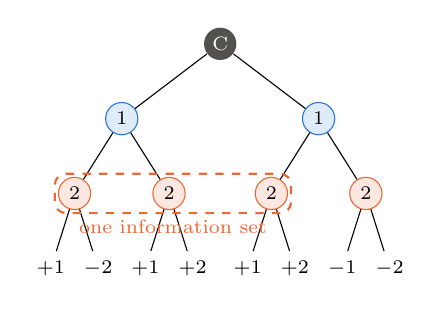
\begin{tikzpicture}[level distance=0.95cm,
   level 1/.style={sibling distance=2.5cm},level 2/.style={sibling distance=1.2cm},level 3/.style={sibling distance=0.6cm},
   every node/.style={font=\scriptsize}]
  \node[circle,fill=ink2,text=white,inner sep=1.5pt] {C}
    child { node[circle,draw=cblue,fill=cblue!15,inner sep=2pt] (a) {1}
       child { node[circle,draw=corange,fill=corange!15,inner sep=2pt] (b1) {2} child{node{$+1$}} child{node{$-2$}} }
       child { node[circle,draw=corange,fill=corange!15,inner sep=2pt] (b2) {2} child{node{$+1$}} child{node{$+2$}} } }
    child { node[circle,draw=cblue,fill=cblue!15,inner sep=2pt] (c) {1}
       child { node[circle,draw=corange,fill=corange!15,inner sep=2pt] (d1) {2} child{node{$+1$}} child{node{$+2$}} }
       child { node[circle,draw=corange,fill=corange!15,inner sep=2pt] (d2) {2} child{node{$-1$}} child{node{$-2$}} } };
  \draw[corange,dashed,thick,rounded corners] ($(b1)+(-0.25,0.25)$) -- ($(d1)+(0.25,0.25)$) -- ($(d1)+(0.25,-0.25)$) -- ($(b1)+(-0.25,-0.25)$) -- cycle;
  \node[corange,font=\scriptsize] at ($(b1)!0.5!(d1)+(0,-0.42)$) {one information set};
\end{tikzpicture}\\[2pt]
{\scriptsize Player 2 sees the action of player 1 but not the deal.}
\end{columns}
\note{
Leduc hold'em is the standard research benchmark. It has a deck of six cards, one private
card each, one public card, and two betting rounds. It has 288 information sets and we use it as our small test problem.\\[3pt]
The size column is the reason the subject exists. Nobody can write down no-limit hold'em. Real systems solve an abstraction
in which similar hands and bet sizes are merged, and then solve subgames like our river again during play.\\[3pt]
We assume perfect recall: a player never forgets what he knew or did. Sizes are from Bowling et al.\ 2015 and Johanson 2013.
Kuhn and Leduc were counted by our code.
}
\end{frame}

% =====================================================================================
\begin{frame}{\tagM\ The sequence form: equilibrium is a linear program}
Give player 1 one variable $x_\sigma$ for each \emph{sequence} $\sigma$ of her own
actions, equal to the product of her probabilities along it. These variables satisfy linear flow constraints
$Ex = e$, $x\ge 0$, and the expected payoff is bilinear in them, $u(x,y) = x^\top A y$.
\begin{block}{Theorem (Koller, Megiddo and von Stengel 1996)}
An equilibrium strategy of player 1 solves
\[\max_{x,\,q}\ f^\top q\quad \text{subject to}\quad A^\top x - F^\top q \ge 0,\quad Ex = e,\quad x\ge 0 ,\]
a linear program whose size is \emph{linear} in the size of the game tree.
\end{block}
So why not call an LP solver? On our river $A$ has 2.9 million nonzeros, because every leaf couples every hand of one
player to every hand of the other, and a good LP code did not finish in 25 minutes. The iteration we describe next
reaches $\MedDCFRExpl$ chips in \MedDCFRTime\ seconds.
\note{
This is the key modelling step. Mixed strategies over the pure strategies of the normal form would have exponentially many
variables. Realisation plans have one variable per sequence, and perfect recall makes the payoff bilinear in them.\\[3pt]
$E$ and $F$ are very sparse, with one row per information set and entries $\pm1$, and they encode flow conservation on a tree.
$A$ is where the poker lives. The program has 17{,}626 unknowns on our river. Say that the dual variables $q$ are the values of the opponent's information sets, and remember them: they are values of information sets, the same quantities
that CFR computes in every iteration. This is how we will warm-start the duals later.\\[3pt]
The LP run used HiGHS through SciPy with default settings on one core and we stopped it after 25 minutes. On the smaller test
problems the LP is perfectly fine: 0.04 s on Leduc and 1.6 s on a small river. The DCFR figure is for \MedDCFRIters\ iterations.
}
\end{frame}

% =====================================================================================
\begin{frame}{\tagM\ Regret matching}
\begin{columns}[T]
\column{0.62\textwidth}
We face the same decision many times. The \emph{regret} $R_T(a)$ of an action is how much better it would have done
than what we played. Regret matching plays each action in proportion to its positive regret.
{\small\[ R_T(a) = \sum_{t=1}^T \big(u_t(a) - u_t(\sigma_t)\big),\quad
   \sigma_{T+1}(a) = \frac{[R_T(a)]^+}{\sum_b [R_T(b)]^+}. \]}
\begin{block}{Theorem (Hart and Mas-Colell 2000)}
The regrets grow only like $\sqrt{T}$: $\ \max_a R_T(a) \le \Delta\sqrt{|A|\,T}$.
\end{block}
When both players of a zero-sum game do this, their \emph{average} strategies converge to an equilibrium.
\column{0.36\textwidth}
\centering
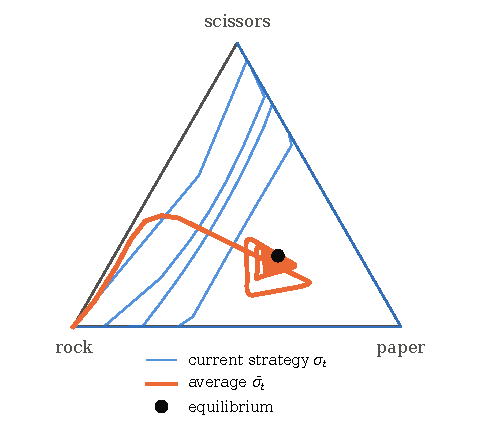
\includegraphics[width=\linewidth]{rm_rps.pdf}\\
{\scriptsize Our computation on a weighted rock-paper-scissors game. The current strategy cycles and the average converges.}
\end{columns}
\note{
Idea of the proof. The regret vector satisfies $\|[R_{T}]^+\|^2 \le \|[R_{T-1}]^+\|^2 + \Delta^2|A|$ because the
cross term $\langle [R_{T-1}]^+, r_T\rangle$ vanishes by the choice of $\sigma_T$: the instantaneous regret is orthogonal to the
current positive regrets. Sum and take square roots. This is Blackwell approachability, and $\Delta$ is the range of the payoffs.\\[3pt]
The folk theorem: if both players have average regret at most $\varepsilon$ then the average strategies are a $2\varepsilon$-equilibrium,
because $\max_{x'} x'^\top A \bar y - \min_{y'} \bar x^\top A y' \le 2\varepsilon$.\\[3pt]
In the figure the limit is $(\frac14,\frac12,\frac14)$.
}
\end{frame}

% =====================================================================================
\begin{frame}{\tagM\ Counterfactual regret minimisation (CFR)}
CFR runs regret matching separately at every information set $I$. The payoff it feeds to each one is the
\textbf{counterfactual value} of an action, which is the expected payoff weighted by the probability that the opponent and
chance lead to $I$, as if the player herself had tried to get there.
\[ v_i(\sigma, I, a) = \sum_{h\in I}\ \pi_{-i}^{\sigma}(h)\sum_{z \sqsupset ha} \pi^{\sigma}(ha\to z)\, u_i(z) \]
\begin{block}{Theorem (Zinkevich, Johanson, Bowling and Piccione 2007)}
The regret of the whole strategy is at most the sum of the local regrets. Therefore the average strategies satisfy
\[ \ex(\bar x_T,\bar y_T) \ \le\ \frac{\Delta\,|\mathcal I|\sqrt{|A|}}{\sqrt T}. \]
\end{block}
One iteration is one pass over the tree, with reach probabilities computed on the way down and values on the way up.
The matrix $A$ is never formed.
\note{
The decomposition is the whole trick. A global regret over an exponentially large strategy space is bounded by a sum of small
local regrets, and each of them is minimised by plain regret matching. This is why CFR scales: the cost of an iteration is linear in the tree
and so is the storage, two numbers for each information set and action.\\[3pt]
In the language of linear algebra, one CFR iteration computes $Ay$ and $A^\top x$ for the current realisation plans by walking the tree.
These are the same two products that any first-order saddle-point method needs.
}
\end{frame}

% =====================================================================================
\begin{frame}{\tagP\tagM\ CFR for poker: one pass for all hands}
In poker the betting is public and only the cards are hidden. At each point of the betting we store
\emph{vectors} indexed by hands, such as the reach probabilities $\pi_1$ and $\pi_2$.
At a leaf the values of all hands come from one matrix-vector product.
\[ v_1 = \text{amount}\cdot B\,\pi_2,\qquad
   B_{ij} = \underbrace{C_{ij}}_{\text{no shared card}}\cdot\begin{cases} 1 & \text{after a fold}\\ \operatorname{sign}(s_i - s_j) & \text{at a showdown}\end{cases} \]
Here $s_i$ is the strength of hand $i$. The matrix $B$ is dense but very structured. Once the hands are sorted by
strength, the sign matrix is all ones below the diagonal and all minus ones above it, and $C$ is the all-ones matrix
minus a sparse correction for hands that share a card.

\medskip
As a result $B\pi$ costs one sort and a running sum, which is $O(n\log n)$ operations and not $n^2$.
\note{
This is the bridge between the tree picture and the implementation. The information sets at a public node are indexed by the
private hand of the player to act, so all information sets at this node form a vector and every CFR operation becomes a vector operation.\\[3pt]
This is also the poker-specific numerical linear algebra. Each terminal block is low rank plus sparse. The fold block is
rank one minus a sparse correction. The showdown block, after sorting, is a sign matrix, which is semiseparable (think of the inverse of
a bidiagonal matrix), times the compatibility mask. The trick is due to Johanson et al.\ 2011.\\[3pt]
The public tree itself is drawn live in the demonstration, so it is not on a slide any more. It has 12 decision points and 21 leaves, and one iteration takes about a millisecond in the browser. Keep in mind that this structure is what a
scalable Newton method would have to exploit, which comes back at the end of the talk.
}
\end{frame}

% =====================================================================================
\begin{frame}{\tagM\ Four variants of one loop}
Modern solvers change how CFR weights the old regrets and how it averages the strategies.

\smallskip
\renewcommand{\arraystretch}{1.15}\small
\begin{tabular}{p{1.5cm}p{6.4cm}p{5.0cm}}
\toprule
method & what changes & a numerical analyst would say \\ \midrule
CFR$^+$ & Negative regrets are reset to zero and later strategies get more weight in the average. & projection onto the nonnegative orthant \\
DCFR & Old regrets and old strategies are multiplied by factors below one. & forgetting factors that damp the transient \\
PCFR$^+$ & The strategy is computed from the regrets plus a prediction of the next regret. & optimism, as in the extragradient method \\ \bottomrule
\end{tabular}

\smallskip
\normalsize The proven rate is still $T^{-1/2}$ for all four. In practice the modern variants are much faster, and we will
now race them against each other on a real hand.
\note{
CFR$^+$ (Tammelin 2014) is what solved limit hold'em. DCFR (Brown and Sandholm 2019) with parameters $(1.5, 0, 2)$ is the default in many solvers:
positive regrets are multiplied by $t^{1.5}/(t^{1.5}+1)$, negative ones by $1/2$, and the average by $(t/(t+1))^2$.
PCFR$^+$ (Farina, Kroer and Sandholm 2021) uses the last instantaneous regret as its prediction and connects regret matching to optimistic mirror descent.\\[3pt]
All four also update the two players in turn, so that the second player already sees the new strategy of the first, which is Gauss-Seidel in place of Jacobi.\\[3pt]
The observed rates are between $T^{-1}$ and $T^{-3/2}$ for the averages, while the last iterate oscillates. Explaining this gap to the
theory is an open question. The rates are still sublinear, and that is the gap our method addresses.
}
\end{frame}

% =====================================================================================
\begin{frame}{\tagP\tagM\ Live demonstration: the river solver table}
\begin{columns}[c]
\column{0.55\textwidth}
\centering
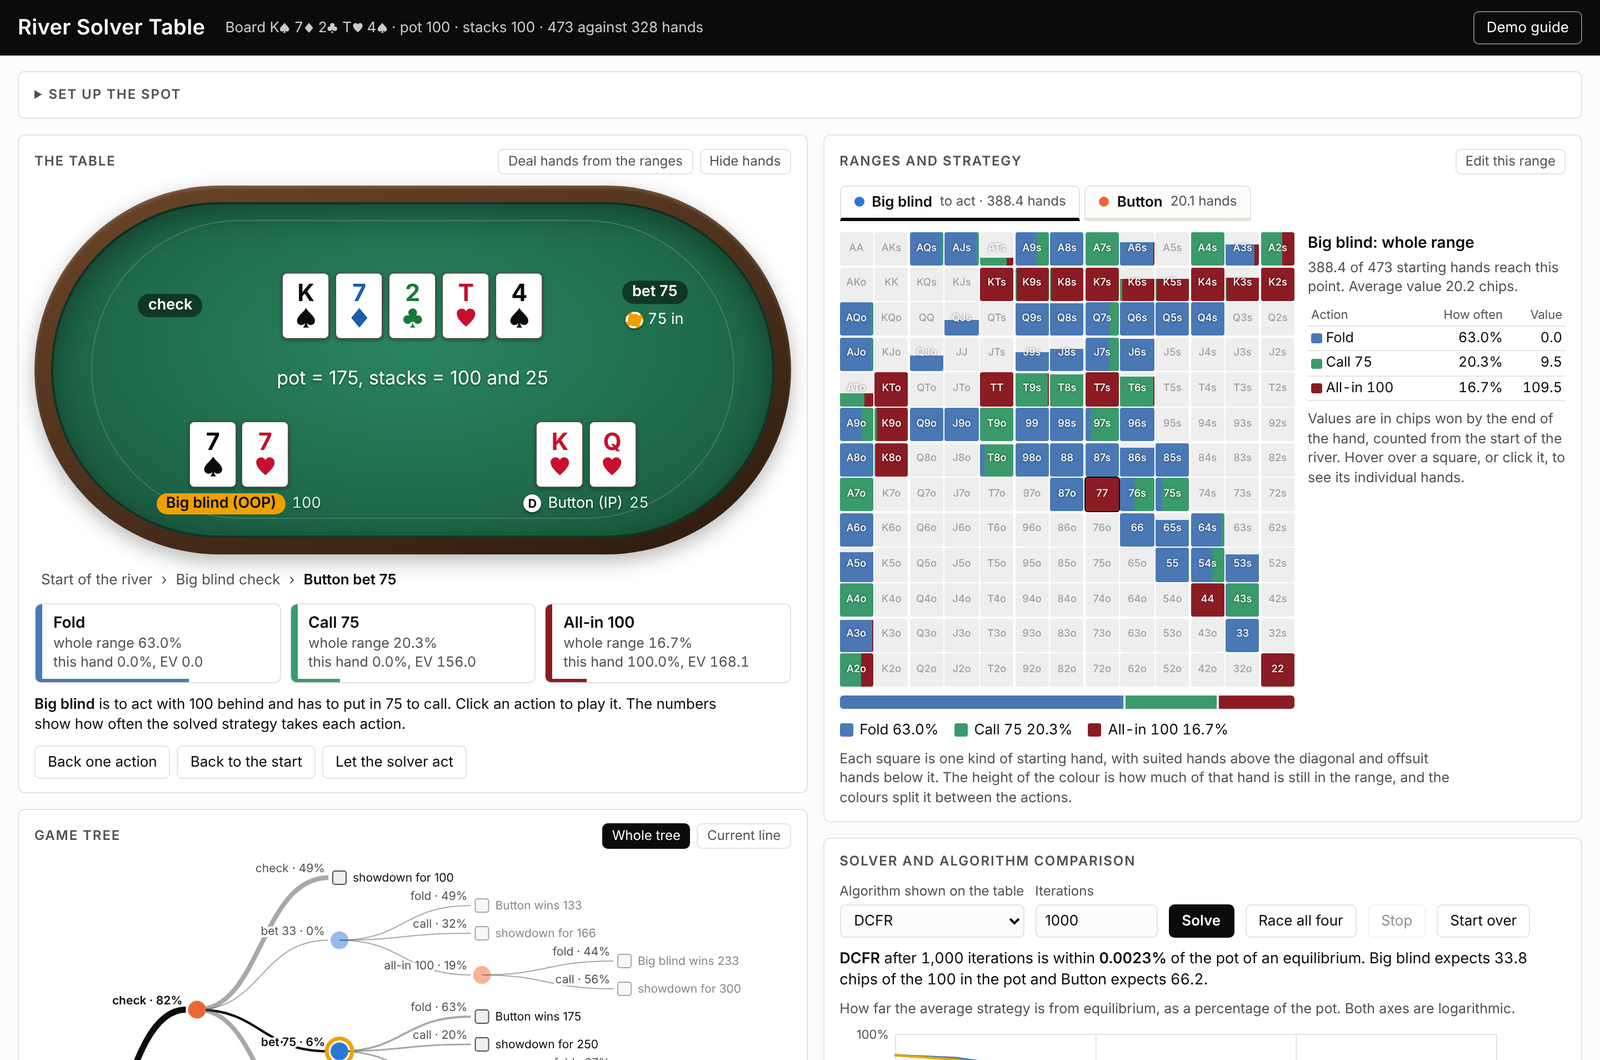
\includegraphics[width=\linewidth]{app_slide.png}
\column{0.43\textwidth}
The page \texttt{app/poker-solver.html} solves our river in the browser. It will answer five questions.
\begin{enumerate}\small\setlength\itemsep{2pt}
\item Which of the four algorithms wins a race?
\item What does the big blind do with each of its 473 hands?
\item How do the ranges and the tree change as the hand is played?
\item Does a hand that mixes get the same value from both actions?
\item Does the solver agree with the pot odds formula?
\end{enumerate}
After that the board, the ranges and the bet sizes are yours to change.
\end{columns}
\note{
Switch to the browser now. The full script with what to click and what to say is in \texttt{app/DEMO\_NOTES.md} (also as a PDF),
and the same steps are in the Demo guide inside the page. Budget twelve minutes.\\[3pt]
Short version of the script. (1) Load the page, which solves the spot with DCFR in two seconds. Point at the table, the grid, the tree and the chart.
(2) Press Race all four. After 1000 iterations CFR is at about 0.11\% of the pot, PCFR$^+$ at 0.009\%, CFR$^+$ at 0.007\% and DCFR at 0.002\%.
(3) Read the big blind's grid: check 82\%, bet a third of the pot 16\%, bet three quarters 2\%. Value bets and bluffs.
(4) Give the big blind three sevens: it checks every time, and after the button bets 75 it raises all-in every time.
(5) After check and bet 75, select ace-nine offsuit: it folds 63\% and calls 37\%, and both actions are worth 0.0 chips.
(6) After the big blind bets 33, the button folds 26\%, and the formula says at most 25\%. After a check and an all-in the big blind folds 68\%, far more than the formula's 50\%.
(7) Change the river card to the nine of hearts and solve again. Then take requests from the audience.\\[3pt]
If the browser fails, the static grids are in \texttt{talk-detailed.pdf}, slides 18 and 19.
}
\end{frame}

% =====================================================================================
\begin{frame}{\tagP\ What the demonstration showed}
\begin{columns}[T]
\column{0.42\textwidth}
The solution reads like poker. Strong hands bet, a few hands with nothing bluff, and the hands in between check.

\medskip
A hand that mixes two actions gets the same value from both. This is complementary slackness.

\medskip
The button defends within 1.5 points of the pot odds formula. The big blind folds much more than the formula says,
because the button's bluffs would still win some showdowns by checking.
\column{0.57\textwidth}
\centering
{\scriptsize\setlength\tabcolsep{3pt}
\input{mdf_table.tex}}\\[6pt]
{\scriptsize Exact equilibrium of our river. Here $s$ is the bet as a fraction of the pot, MDF is $1/(1+s)$, and a jam is an all-in bet.}
\end{columns}
\note{
This is a consistency check of the whole pipeline. When the big blind bets, the button defends 74.3\% against 75.2\%, 55.8\% against
57.1\% and 49.1\% against 50.0\%, so the toy formula is almost exact. When the button bets after a check, the big blind folds much
more. We checked that the button's weakest betting hands mix between checking and going all-in, so the indifference that fixes
the defence frequency is ``value of the all-in equals value of checking, which is positive'' and not ``value of the all-in equals zero''.\\[3pt]
The numbers in the table come from the exact equilibrium computed by the method of the next part, so they can differ in the last digit from what the
browser showed after 1000 iterations.
}
\end{frame}

% =====================================================================================
\begin{frame}{\tagM\ Why push the precision further?}
\begin{columns}[T]
\column{0.58\textwidth}
Practical solvers stop at about 0.1\% of the pot, and for a human studying a hand that is plenty.

\medskip
More digits matter when a program stitches many small solves together and their errors add up, when we ask exactly which
hands mix, and when research needs a ground truth with a certificate.

\medskip
For a numerical analyst, CFR is a first-order method on a nonsmooth and degenerate problem. It is
robust and cheap, and its tail is sublinear. The classical cure for a slow tail is a \alert{local method of higher
order}, started from a good point.
\column{0.4\textwidth}
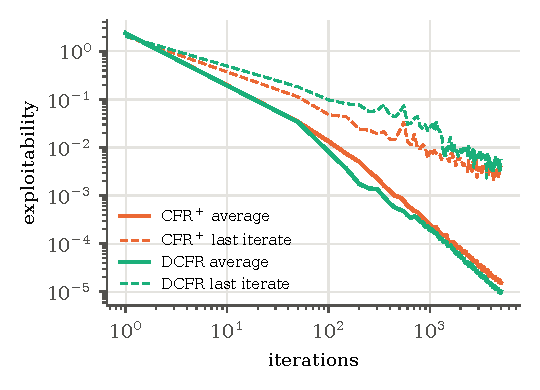
\includegraphics[width=\linewidth]{avg_vs_last.pdf}\\
{\scriptsize Our computation on Leduc. Only the average converges, and each extra digit costs about ten times more iterations.}
\end{columns}
\note{
Make the case without overselling. Precision matters for machines (solving subgames again, evaluation) and for science
(knowing the exact equilibrium, for example the exact bluffing frequencies, or whether a hand mixes at all).\\[3pt]
The analogy for this audience: CFR is like a stationary iterative method. It is fantastic for the first
digits and hopeless for the last ones, and the obvious idea is to switch to a Newton-type method near the solution.\\[3pt]
Numbers for Leduc: CFR$^+$ reaches $\LeducCFRplusLong$ after 50{,}000 iterations and \LeducCFRplusLongTime\ seconds. The curves are on a backup slide.
}
\end{frame}

% =====================================================================================
\begin{frame}{\tagO\ Step 1: write the equilibrium as a variational inequality}
Collect both strategies and both vectors of information-set values in one unknown $z = (x, y, p, q)$. An
equilibrium is a point that satisfies the optimality conditions of both players' linear programs.
\[
\begin{aligned}
 0\le x \ &\perp\ E^\top p - A y \ \ge 0, & Ex &= e,\\
 0\le y \ &\perp\ A^\top x - F^\top q \ \ge 0, & Fy &= f.
\end{aligned}
\]
These conditions have the form $w = Mz + b$ with a matrix that is \textbf{skew-symmetric}.
\[ M = \begin{pmatrix} 0 & -A & E^\top & 0\\ A^\top & 0 & 0 & -F^\top\\ -E & 0 & 0 & 0\\ 0 & F & 0 & 0\end{pmatrix},
   \qquad M + M^\top = 0 . \]
Skew symmetry makes the problem monotone. It also means that the solutions form a polyhedron and
not a single point, so Newton's method cannot be applied directly. CFR gives a starting point for all of $z$ for free.
\note{
This is a mixed linear complementarity problem. The reduced cost $E^\top p - Ay$ of a sequence is its counterfactual
regret scaled by reach, and complementarity says ``play only actions with zero regret''. So CFR and this system talk
about the same quantities: the CFR average strategies are $x$ and $y$, and its best-response values are $p$ and $q$.\\[3pt]
Skewness: the $x$-$y$ block is the zero-sum coupling. The $(x,p)$ and $(y,q)$ blocks are pairs of constraints and multipliers, arranged
with signs so that $M^\top = -M$.\\[3pt]
Non-uniqueness is already visible in Kuhn poker, where the equilibria form a one-parameter family (backup slide).\\[3pt]
If asked what we tried first: Anderson acceleration of the CFR$^+$ map, vector extrapolation of the averages, and Levenberg-Marquardt on the
optimality system. None of them beat DCFR on Leduc. The CFR map is piecewise linear with non-isolated fixed points, and the acceleration theory needs a smooth contraction.
The details are in \texttt{talk-detailed.pdf}.
}
\end{frame}

% =====================================================================================
\begin{frame}{\tagO\ Step 2: the proximal point method makes each problem well posed}
We add a small multiple of the identity. Given $z^k$, the next iterate $z^{k+1}$ solves the same conditions with
\[ w_\rho(z) = (M + \rho I)\,z + b - \rho\, z^{k} . \]
\begin{columns}[T]
\column{0.56\textwidth}
Since $d^\top(M+\rho I)d = \rho\|d\|^2$, the matrix $M+\rho I$ is positive definite and each regularised problem
has exactly one solution.

\medskip
\textbf{Theorem (Rockafellar 1976, Luque 1984).} The iterates converge to a solution of the original problem for every
$\rho>0$. For a polyhedral problem the rate is linear, with a factor that tends to zero with $\rho$.

\medskip
A small $\rho$ gives a fast outer loop and badly conditioned inner problems.
\column{0.41\textwidth}
\begin{block}{Our computation on Leduc with $\rho = 10^{-5}$}
\small The residual after each outer step:\\[2pt]
$3.4\!\times\!10^{-2} \to 4.8\!\times\!10^{-6} \to 3.3\!\times\!10^{-9}$\\ $\to 6.9\!\times\!10^{-12} \to 2.0\!\times\!10^{-14}$\\[3pt]
About three digits for each step.
\end{block}
\end{columns}
\note{
The proximal term fixes the non-uniqueness. Each subproblem has exactly one solution, so Newton's method has a well defined and
nonsingular target. For polyhedral monotone problems the inverse operator is upper Lipschitz (Robinson 1981), which gives linear
convergence of the proximal point method with a factor that tends to zero as $\rho\to0$.\\[3pt]
The trade-off is the whole story of the last part of the talk. A small $\rho$ makes the outer loop fast and the inner problems
nearly as ill posed as the original one, since $\|(M+\rho I)^{-1}\|\le 1/\rho$. There is a backup slide with the rate.
}
\end{frame}

% =====================================================================================
\begin{frame}{\tagO\ Step 3: Newton's method on a piecewise-linear equation}
Each regularised problem can be written as one equation. For every action, either its probability is zero or its
reduced cost is zero, and that is the same as $\min\big(x_i,\ w_\rho(z)_i\big)=0$.

\medskip
A Newton step for this equation guesses which actions are dropped, imposes indifference on all the others, and solves
one linear system. Its matrix has the form $V = D_a + D_b(M+\rho I)$ with nonnegative diagonal matrices $D_a$ and $D_b$.
\begin{block}{Lemma. Every such $V$ with $D_a+D_b$ positive definite is nonsingular.}
\small Suppose $Vd=0$ and put $u = (M+\rho I)d$. Row $i$ reads $(D_a)_{ii}d_i + (D_b)_{ii}u_i = 0$ with nonnegative coefficients
that are not both zero, so $d_i u_i \le 0$. Hence $\rho\|d\|^2 = d^\top u = \sum_i d_i u_i \le 0$, and $d=0$. \hfill$\square$
\end{block}
If the guess of the dropped actions is right, a single step gives the \emph{exact} solution. If it is wrong there is no
global guarantee, so the method needs a good starting guess.
\note{
The min-function turns complementarity into a piecewise-linear equation. Semismooth Newton on it is exactly the
primal-dual active-set method (Hinterm\"uller, Ito and Kunisch 2002). The lemma is the reason
for the proximal term: without $\rho$ we have $d^\top M d = 0$ and the argument fails. Newton matrices of the unregularised problem
are singular at degenerate solutions, which is what we saw with Levenberg-Marquardt.\\[3pt]
The lemma also covers the Fischer-Burmeister reformulation, which has a smooth merit function and a globally convergent damped Newton method.
We tried it first. It worked on Leduc and on a small river with 50 to 70 linear solves, but on the river of the demonstration it
took steps of size $10^{-3}$ for dozens of iterations. That pushed us to the interior-point start on the next slide.
}
\end{frame}

% =====================================================================================
\begin{frame}{\tagO\ Step 4: making it robust and fast}
\begin{columns}[T]
\column{0.55\textwidth}
\textbf{A robust start.} The first regularised problem is the hardest. We solve it with an interior-point method
started at the CFR point. Its solution tells us which actions are dropped, and from there the Newton steps land
exactly on the solution. Every later problem needs only one to three linear solves.

\medskip
\textbf{Fast linear algebra.} After a change of signs in half of the rows, every linear system is symmetric and
\emph{quasi-definite}. By a theorem of Vanderbei, such a matrix has an $LDL^\top$ factorisation for every ordering of
the unknowns, so we can order for sparsity alone and never pivot.
\column{0.42\textwidth}
\begin{block}{One factorisation, in seconds}
\footnotesize
\begin{tabular}{@{}l@{\ \ }c@{\ \ }c@{}}
& small river & our river\\ \midrule
general sparse LU & 0.11 & 25\\
quasi-definite $LDL^\top$ & 0.04 & 7.6
\end{tabular}
\end{block}
\vspace{4pt}
{\small The whole solve from the CFR point to a residual of $10^{-13}$ takes \LeducSolves\ linear solves on Leduc and
\SmallSolves\ on the small river.}
\end{columns}
\note{
The first problem is the hardest because many actions enter or leave the support. The division of labour mirrors what commercial LP solvers do, interior point and then crossover to a vertex, but inside a proximal
loop and with a game-theoretic warm start. We use Mehrotra's predictor-corrector method. In our runs the interior-point phase took 6 to 8 factorisations on Leduc and the small
river, the crossover a few active-set steps, and every later proximal step 1 to 3 steps. We use $\rho=10^{-5}$ throughout.\\[3pt]
Quasi-definite means the block form $\begin{psmallmatrix} P & B\\ B^\top & -N\end{psmallmatrix}$ with $P$ and $N$ positive definite, after grouping $(x,q)$ and $(y,p)$.
Vanderbei's theorem (1995) lets us choose a fill-reducing ordering before seeing the numbers, which is the same reason interior-point
codes like quasi-definite systems. The timings compare SuperLU with QDLDL on one core.\\[3pt]
A caveat: with only $\pm10^{-5}$ on the diagonal, as in the pure active-set systems, static pivoting is too unstable. There we use a
pivoted sparse LU, which is cheap because the active-set system lives on the support only.
}
\end{frame}

% =====================================================================================
\begin{frame}{\tagP\tagO\ Step 5: restrict to the support, solve exactly, then verify}
\begin{columns}[T]
\column{0.54\textwidth}
On larger hands the method so far fails. Many actions are never played and many positions are never
reached, and in those directions the set of equilibria is \emph{flat}. A point with a tiny residual can be far
from a solution, and the Newton step guesses the wrong dropped actions.

\medskip
The cure is to remove those directions. We keep only the actions that DCFR plays with probability above $10^{-3}$ and
solve this smaller problem exactly.

\medskip
Then we check the answer in the full game. If a removed action would have been profitable we put it back and solve again.
\column{0.43\textwidth}
\begin{block}{The complete method}
\small
\begin{enumerate}\setlength\itemsep{2pt}
\item DCFR for a few thousand iterations
\item keep the actions that it uses
\item solve the restricted problem to machine precision
\item compute exact best responses in the full game
\item add back any profitable action and return to 3
\end{enumerate}
\end{block}
{\small Step 4 is a certificate. The final exploitability is measured in the full game and not assumed.}
\end{columns}
\note{
The verification loop is column generation, the same idea as the double-oracle algorithms for games (McMahan, Gordon and Blum 2003,
Bo\v{s}ansk\'y et al.\ 2014). We also keep only the positions that both players can still reach with the kept actions. What is new is the combination with a support predicted by CFR and an exact
second-order solve of the restricted problem.\\[3pt]
Poker helps here. Equilibria are mostly pure, because mixing happens only at indifference. In the exact Leduc equilibrium about half of the
reachable pairs of information set and hand play a single action, and on the small river 71\%. About half of all sequences are outside the
support, and the dense payoff blocks shrink to the hands that actually reach each leaf.\\[3pt]
On our problems Leduc needed 2 rounds, the small river 1, and the river of the demonstration 3, with 16 actions added back in total. The restricted
problem had about 35\% of the unknowns of the full one.
}
\end{frame}

% =====================================================================================
\begin{frame}{\tagO\ Result on the benchmark game, Leduc hold'em}
\begin{columns}[c]
\column{0.6\textwidth}
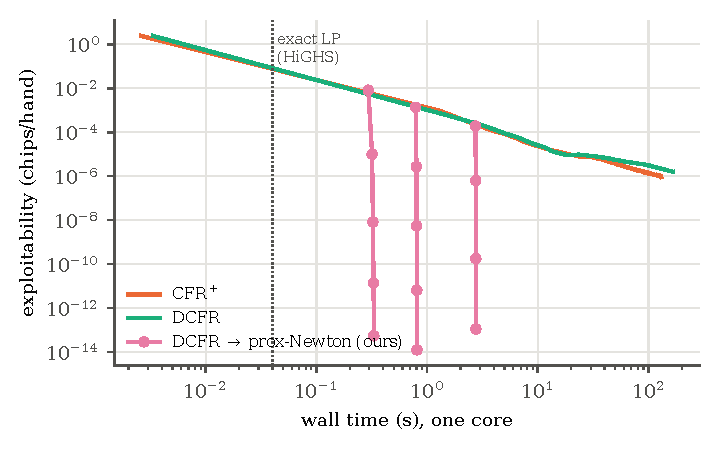
\includegraphics[width=\linewidth]{hybrid_leduc.pdf}
\column{0.38\textwidth}
Each pink curve starts where a short DCFR run stopped and drops straight down to machine precision.

\medskip
From \SuppLeducWarm\ DCFR iterations our method reaches $\SuppLeducExpl$ in \alert{\SuppLeducTime\
seconds}. CFR$^+$ is at $\LeducCFRplusLong$ after \LeducCFRplusLongTime\ seconds.

\medskip
Leduc is tiny and an LP solver needs 0.04 seconds. What matters is the shape of the curves.
\end{columns}
\note{
Each pink curve starts where the DCFR warm start stopped, after 100, 300 or 1000 iterations. The points are verification rounds.
Starting from 100 DCFR iterations is enough and costs one extra round. Starting later only costs DCFR time. The run used \SuppLeducRounds\ rounds and \SuppLeducSolves\ linear solves.\\[3pt]
The value of the game that we obtain, $-0.085606424078\ldots$ chips for the first player, agrees with the LP in all printed digits.\\[3pt]
Be upfront about the LP. Leduc has 964 unknowns and a simplex method finishes in 40 ms. The question is what happens when
the LP does not fit, which is the next slide.
}
\end{frame}

% =====================================================================================
\begin{frame}{\tagO\ Result on the river from the demonstration}
\begin{columns}[T]
\column{0.52\textwidth}
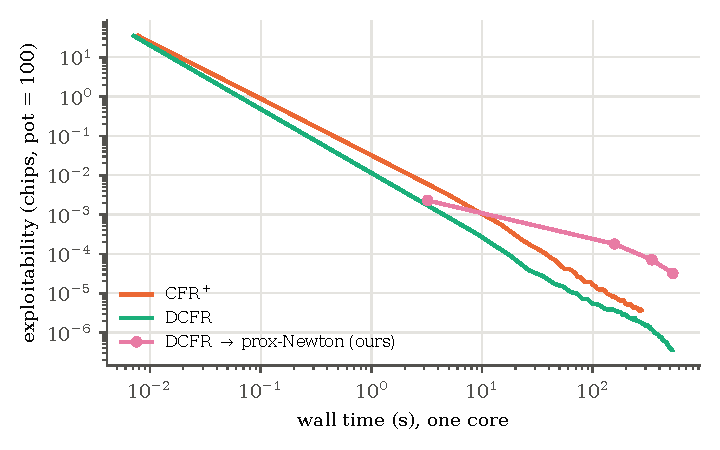
\includegraphics[width=\linewidth]{hybrid_medium.pdf}\\
{\scriptsize 473 against 328 hands and 17{,}626 unknowns. The points are verification rounds.}
\column{0.46\textwidth}
Our method runs DCFR for \SuppMedWarm\ iterations and then needs \SuppMedRounds\ rounds on a problem with \SuppMedFrac\%
of the unknowns. It reaches \alert{$\SuppMedExpl$ chips in \SuppMedTime\ seconds}.

\medskip
At that moment DCFR alone is at $\MedDCFRAtSuppTime$, and after \MedDCFRLongTwoIters\ iterations and \MedDCFRLongTwoTime\
seconds it is at $\MedDCFRLongTwoExpl$.

\medskip
Without the restriction to the support the Newton finish \emph{loses} to DCFR on this hand. The LP solver did not finish in 25
minutes.
\end{columns}
\note{
This is the slide that took the longest to earn. The first version of the method, Newton on the full sequence-form problem, worked
on Leduc and the small river and lost to DCFR here, with $\MedHybExpl$ after \MedHybTime\ seconds. The crossover from the interior point kept landing on a wrong active set,
because the equilibrium set is flat in directions that do not matter, and with
$\rho=10^{-5}$ an error in those directions is amplified by $1/\rho$. A larger $\rho$ made the active-set steps work and the
outer loop crawl. Anderson acceleration of the proximal map helped, to $8\times10^{-7}$ in 8 minutes, and then stalled.\\[3pt]
Restricting to the support predicted by CFR and verifying afterwards removes exactly those directions. \SuppMedAdded\ actions were added back in total.
Starting from 1{,}000 DCFR iterations gives $\SuppMedOneKExpl$ in \SuppMedOneKTime\ seconds.\\[3pt]
On the small river (147 against 139 hands) the method reaches $\SuppSmallExpl$ in \SuppSmallTime\ seconds, DCFR is at $\SmallDCFRExpl$ after \SmallDCFRTime\ seconds, and the LP takes 1.6 seconds. This is on a backup slide.
}
\end{frame}

% =====================================================================================
\begin{frame}{\tagO\ Where it stops winning, and what is open}
\begin{block}{Full ranges: all 1{,}081 hands for both players, 47{,}568 unknowns}
\small The restricted problem still has 43\% of the unknowns and one factorisation takes about 10 seconds. After 80 minutes our
method is at $4.1\times10^{-6}$ chips. DCFR reaches $9.5\times10^{-6}$ in 10 minutes. \textbf{Here CFR wins.}
\end{block}

\medskip
The bottleneck is the linear algebra. Each payoff block is dense, but it is a sorted sign matrix plus a sparse correction,
and a product with it costs $O(n\log n)$. A Newton--Krylov step would then cost only a few CFR iterations, provided we can
find a good preconditioner for systems of the form ``diagonal plus skew''. We think this is the most promising open problem,
and it is a problem in numerical linear algebra.

\medskip
Two further directions are a better prediction of the support from the CFR regrets, which would save verification rounds,
and the use of exact solves inside programs that play in real time.
\note{
The run with full ranges is the honest boundary of the method as implemented. The restriction still removes more than half of the
unknowns, but each factorisation of the remaining system with 20{,}000 unknowns takes about 10 seconds because the payoff blocks between
the hands that remain in play are dense. The first round needed 201 solves and 50 minutes, the second 116, and the second did not
reach machine precision (the proximal loop stalled at a residual of $5\times10^{-7}$).
DCFR does 40{,}000 iterations in 10 minutes.\\[3pt]
The research directions are natural ones for this club. The first is the one I would bet on: the structure that
makes CFR fast (sorting, running sums, card-removal corrections) is exactly the structure that a fast direct or preconditioned iterative
solver for the Newton systems would need. Hierarchical factorisations of the blocks are a candidate.
}
\end{frame}

% =====================================================================================
\begin{frame}{\tagO\ What is new here, and what is not}
The ingredients are classical: the sequence form, the proximal point method, semismooth Newton,
interior point with crossover, quasi-definite factorisations and the CFR family.

\medskip
The closest work is by Yang, Gao, Lin and Kroer (2025), who use a semismooth Newton method for \emph{matrix} games after a
first-order warm start.

\medskip
What we add is a second-order finish that works directly on the sequence form of a poker game. It has four parts:
\begin{itemize}\setlength\itemsep{0pt}
\item the skew formulation with a proximal term, which gives nonsingular Newton matrices by a one-line proof,
\item a warm start for both the strategies and the values taken from CFR,
\item the restriction to the support predicted by CFR, which removes the flat directions,
\item and the verification by exact best responses in the full game.
\end{itemize}
\note{
Be precise about novelty. The general idea of a first-order warm start followed by semismooth Newton for zero-sum games was proposed
for matrix games by Yang, Gao, Lin and Kroer in December 2025 (arXiv 2512.12910). Their Newton system lives on the normal form, they use
Douglas-Rachford splitting and a PRM$^+$ warm start, and they do not treat the structure of extensive-form games.\\[3pt]
To our knowledge no solver based on CFR hands over to a second-order method for the last digits. Early work solved small abstracted games exactly as linear programs (Gilpin and Sandholm 2005). The commercial and research poker solvers that we know of
(PioSolver, GTO+, Libratus, DeepStack) are first-order.
}
\end{frame}

% =====================================================================================
\begin{frame}{Takeaways}
A poker equilibrium is the solution of a structured saddle-point problem, and the sequence form turns it into a linear program
whose size is linear in the game tree.

\medskip
CFR is regret matching at every information set. It never forms the matrix, its proven rate is $T^{-1/2}$, and its modern
variants are much faster in practice, as the race in the browser showed.

\medskip
The output is readable poker: value bets, bluffs, traps and a defence that follows the pot odds.

\medskip
Read as a skew variational inequality, the same problem can be finished by a proximal Newton method. The obstacle is the
flatness of the equilibrium set, and restricting to the support that CFR predicts removes it. On our river this gives
an exploitability of $10^{-12}$ in about two minutes, where DCFR alone is at $10^{-6}$. With full ranges the linear algebra becomes the
bottleneck and CFR wins again.

\medskip
{\small The solver, the interactive page, the benchmarks and these slides are at \texttt{github.com/dwangnumbers/Poker-Solver}.}
\note{
End with the invitation. The open problem on the earlier slide is a natural one for this club: a preconditioner for
shifted skew systems whose off-diagonal blocks are a sorted sign matrix plus a sparse correction.\\[3pt]
If there is time left, go back to the browser and take requests: another board, another range, other bet sizes.
}
\end{frame}

% =====================================================================================
\begin{frame}{Main references}
\footnotesize
\begin{itemize}\setlength\itemsep{1pt}
\item D.~Koller, N.~Megiddo, B.~von Stengel. Efficient computation of equilibria for extensive two-person games. \emph{Games Econ.\ Behav.} 14 (1996).
\item M.~Zinkevich, M.~Johanson, M.~Bowling, C.~Piccione. Regret minimization in games with incomplete information. \emph{NeurIPS} 2007.
\item N.~Brown, T.~Sandholm. Solving imperfect-information games via discounted regret minimization. \emph{AAAI} 2019.
\item R.~T. Rockafellar. Monotone operators and the proximal point algorithm. \emph{SIAM J.\ Control Optim.} 14 (1976).
\item M.~Hinterm\"uller, K.~Ito, K.~Kunisch. The primal-dual active set strategy as a semismooth Newton method. \emph{SIAM J.\ Optim.} 13 (2002).
\item R.~J. Vanderbei. Symmetric quasidefinite matrices. \emph{SIAM J.\ Optim.} 5 (1995).
\item D.~Yang, Y.~Gao, T.~Lin, C.~Kroer. A direct second-order method for solving two-player zero-sum games. arXiv:2512.12910 (2025).
\end{itemize}
The complete list of references is in \texttt{talk-detailed.pdf}.
\end{frame}

% =====================================================================================
\appendix
\begin{frame}{Backup: Kuhn poker, where the equilibrium is not unique}
\begin{columns}[T]
\column{0.55\textwidth}
Kuhn poker uses the three cards \pcard[0.8]{J}{s}\,\pcard[0.8]{Q}{s}\,\pcard[0.8]{K}{s}. Each player puts in one chip and gets one card, and
there is a single bet of one chip.

\medskip
Its equilibria form a one-parameter family. The first player bets the jack as a bluff with any probability
$\alpha$ between 0 and $\tfrac13$, and bets the king with probability $3\alpha$. The value of the game is $-\tfrac1{18}$.

\medskip
The set of equilibria is a polytope and not a point, and any method has to cope with that.
\column{0.42\textwidth}
\begin{block}{Our computation}
\small
The Newton finish returns $\alpha = 0.198$ and bets the king with probability $0.593 = 3\alpha$.\\[2pt]
Value $-0.0555\ldots = -1/18$.\\[2pt]
Exploitability $1.1\times10^{-16}$.
\end{block}
\end{columns}
\note{Kuhn poker is the poker analogue of a two by two test matrix. Jacobians at a solution are
singular, and the proximal term picks one member of the family.}
\end{frame}

\begin{frame}{Backup: the first-order methods on Leduc hold'em}
\begin{columns}[c]
\column{0.58\textwidth}
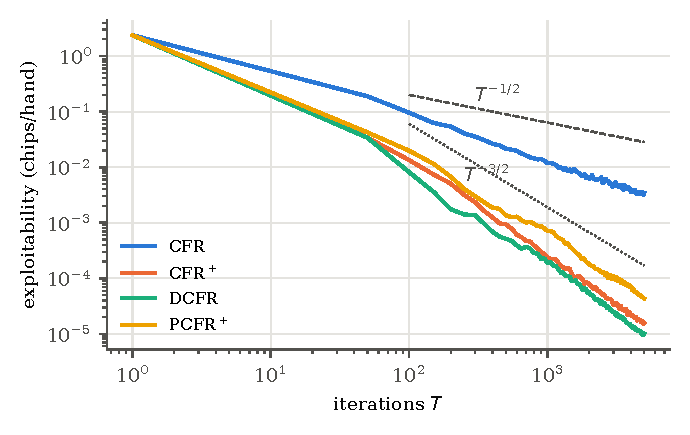
\includegraphics[width=\linewidth]{conv_leduc_iters.pdf}
\column{0.4\textwidth}
The curves show the exploitability of the average strategy for our implementation.

\medskip
After 5{,}000 iterations and \LeducDCFRfiveTime\ seconds DCFR reaches $\LeducDCFRfive$. After 50{,}000 iterations and
\LeducCFRplusLongTime\ seconds CFR$^+$ reaches $\LeducCFRplusLong$ and DCFR $\LeducDCFRLong$.

\medskip
Each extra digit costs about ten times more iterations.
\end{columns}
\note{Exploitability is in chips per hand, and the antes in Leduc are 1 chip.}
\end{frame}

\begin{frame}{Backup: a small river, and every linear solve of one exact solve}
\begin{columns}[c]
\column{0.5\textwidth}
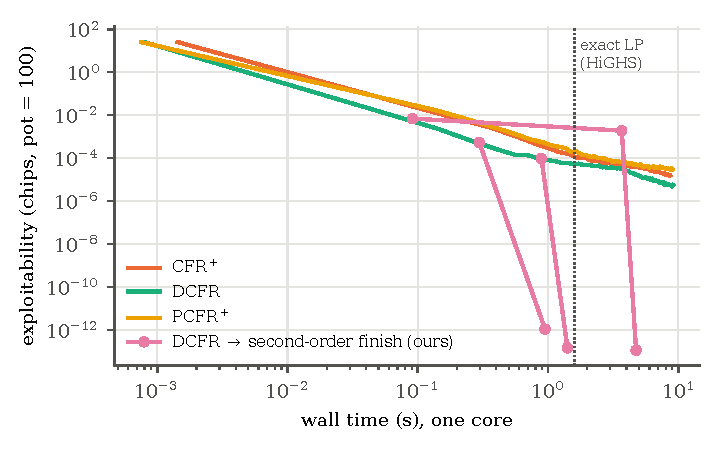
\includegraphics[width=\linewidth]{hybrid_small.pdf}
\column{0.48\textwidth}
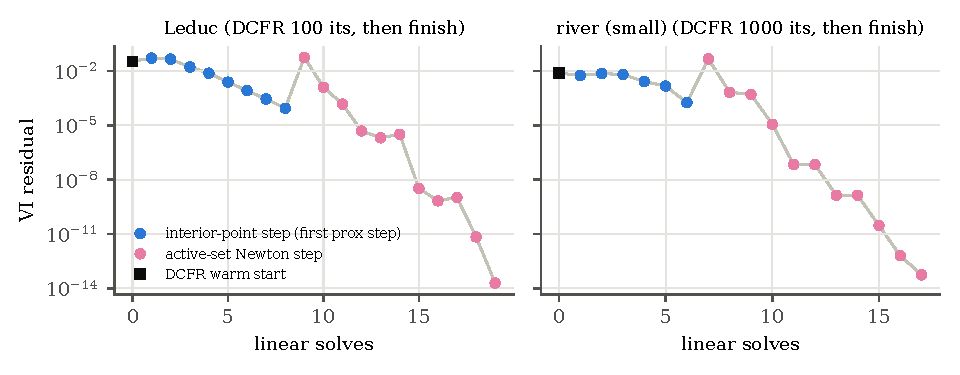
\includegraphics[width=\linewidth]{newton_inner.pdf}
\end{columns}
\medskip
\small On the left is a river with 147 against 139 hands. Our method reaches $\SuppSmallExpl$ chips in \SuppSmallTime\ seconds, DCFR is at
$\SmallDCFRExpl$ after \SmallDCFRTime\ seconds, and the LP takes 1.6 seconds. On the right is the residual after every linear solve. The blue
points are interior-point iterations and the pink points are Newton steps.
\note{The crossover lands on the exact solution of the first regularised
subproblem, whose residual is $\rho\|z^1-z^0\|$, hence the jump. After that each proximal step is solved exactly in one to three steps.}
\end{frame}

\begin{frame}{Backup: the rate of the proximal point method, and why flat equilibria hurt}
The proximal step is the resolvent of a maximal monotone operator $T$, so the iterates move monotonically towards the solution set $Z$.

\medskip
If $T^{-1}$ is upper Lipschitz at $0$ with modulus $a$, which holds for polyhedral problems, then
\[ \operatorname{dist}(z^{k+1}, Z) \ \le\ \frac{a\rho}{\sqrt{1 + a^2\rho^2}}\ \operatorname{dist}(z^k, Z). \]
The modulus $a$ measures how far a point with a small residual can be from $Z$. It is large when the equilibrium set is flat,
that is, when many hands have actions that barely matter.

\medskip
A fast outer loop needs $\rho$ much smaller than $1/a$. But $\|(M+\rho I)^{-1}\|\approx 1/\rho$ then makes the active set of each
subproblem fragile. On Leduc we observe a factor of about $10^{-3}$ for each step at $\rho=10^{-5}$. On the full river of the demonstration no
value of $\rho$ gave both, and the restriction to the support removes the flat directions instead.
\note{Backup for questions about the outer loop. Rockafellar 1976, Luque 1984, Robinson 1981.}
\end{frame}

\end{document}
"
%  This is the simplified deck that goes with the live demonstration (../app). The longer version is talk-detailed.tex.
%  Every number marked "we computed" comes from ../solver (see numbers.tex, generated by gen_numbers.py)
% =====================================================================================
\providecommand\notesmode{0}
\ifnum\notesmode=1 \PassOptionsToClass{handout}{beamer}\fi
\documentclass[10pt,aspectratio=169]{beamer}
\usetheme[progressbar=frametitle,numbering=fraction,block=fill]{metropolis}
\ifnum\notesmode=1
  \setbeameroption{show only notes}
\fi
\usepackage[T1]{fontenc}
\usepackage{lmodern}
\usepackage{amsmath,amssymb,mathtools}
\usepackage{booktabs}
\usepackage{xcolor}
\usepackage{tikz}
\usetikzlibrary{arrows.meta,positioning,calc,shapes.geometric,fit,backgrounds,decorations.pathreplacing}
\usepackage{graphicx}
\usepackage{fancyvrb}
\graphicspath{{../figs/}}
\newcommand{\LeducDCFRfive}{1.0\times 10^{-5}}
\newcommand{\LeducDCFRfiveTime}{14}
\newcommand{\LeducCFRplusLong}{9.2\times 10^{-7}}
\newcommand{\LeducCFRplusLongTime}{130}
\newcommand{\LeducDCFRLong}{1.6\times 10^{-6}}
\newcommand{\LeducHybWarm}{100}
\newcommand{\LeducHybTime}{0.33}
\newcommand{\LeducHybExpl}{5.5\times 10^{-14}}
\newcommand{\LeducHybOuter}{4}
\newcommand{\LeducHybNewton}{19}
\newcommand{\SmallDCFRTime}{9}
\newcommand{\SmallDCFRIters}{30{,}000}
\newcommand{\SmallDCFRExpl}{5.4\times 10^{-6}}
\newcommand{\SmallHybTime}{1.9}
\newcommand{\SmallHybExpl}{3.9\times 10^{-14}}
\newcommand{\SmallHybNewton}{17}
\newcommand{\SmallHybOuter}{6}
\newcommand{\MedDCFRTime}{16}
\newcommand{\MedDCFRExpl}{1.3\times 10^{-4}}
\newcommand{\MedDCFRIters}{5{,}000}
\newcommand{\MedHybTime}{528}
\newcommand{\MedHybExpl}{3.2\times 10^{-5}}
\newcommand{\MedHybOuter}{3}
\newcommand{\MedDCFRLongExpl}{1.8\times 10^{-6}}
\newcommand{\MedDCFRLongTime}{282}
\newcommand{\MedDCFRLongTwoExpl}{3.6\times 10^{-7}}
\newcommand{\MedDCFRLongTwoTime}{520}
\newcommand{\MedDCFRLongTwoIters}{190{,}000}
\newcommand{\MedCFRpLongExpl}{3.8\times 10^{-6}}
\newcommand{\LeducSolves}{19}
\newcommand{\LeducIPM}{8}
\newcommand{\LeducFinishTime}{0.04}
\newcommand{\LeducWarmTime}{0.29}
\newcommand{\SmallSolves}{17}
\newcommand{\SmallIPM}{6}
\newcommand{\SmallFinishTime}{1.58}
\newcommand{\SmallWarmTime}{0.30}
\newcommand{\LeducPure}{49}
\newcommand{\LeducSupport}{59}
\newcommand{\LeducN}{964}
\newcommand{\SmallPure}{71}
\newcommand{\SmallSupport}{52}
\newcommand{\SmallN}{2{,}864}
\newcommand{\SuppLeducTime}{0.30}
\newcommand{\SuppLeducExpl}{6.8\times 10^{-14}}
\newcommand{\SuppLeducRounds}{2}
\newcommand{\SuppLeducWarm}{100}
\newcommand{\SuppLeducSolves}{26}
\newcommand{\SuppSmallTime}{0.95}
\newcommand{\SuppSmallExpl}{1.1\times 10^{-12}}
\newcommand{\SuppSmallRounds}{1}
\newcommand{\SuppSmallWarm}{1{,}000}
\newcommand{\SuppSmallSolves}{16}
\newcommand{\SuppMedTime}{131}
\newcommand{\SuppMedExpl}{2.8\times 10^{-12}}
\newcommand{\SuppMedRounds}{3}
\newcommand{\SuppMedWarm}{3{,}000}
\newcommand{\SuppMedSolves}{163}
\newcommand{\SuppMedFrac}{34}
\newcommand{\SuppMedAdded}{16}
\newcommand{\MedDCFRAtSuppTime}{3.9\times 10^{-6}}
\newcommand{\MedDCFRAtSuppIters}{47{,}490}
\newcommand{\SuppMedOneKTime}{152}
\newcommand{\SuppMedOneKExpl}{3.8\times 10^{-12}}


% ---------- palette (validated categorical slots + inks) ----------
\definecolor{cblue}{HTML}{2A78D6}
\definecolor{corange}{HTML}{EB6834}
\definecolor{caqua}{HTML}{1BAF7A}
\definecolor{cyellow}{HTML}{EDA100}
\definecolor{cmagenta}{HTML}{E87BA4}
\definecolor{ink}{HTML}{0B0B0B}
\definecolor{ink2}{HTML}{52514E}
\definecolor{paper}{HTML}{FCFCFB}
\definecolor{lightblue}{HTML}{CDE2FB}
\definecolor{lightgray}{HTML}{E4E3DF}
\definecolor{felt}{HTML}{1F6B4A}
\definecolor{suitred}{HTML}{C8102E}
\definecolor{suitblue}{HTML}{1C5CAB}
\definecolor{suitgreen}{HTML}{147A3A}
\setbeamercolor{normal text}{fg=ink,bg=paper}
\setbeamercolor{alerted text}{fg=corange}
\setbeamercolor{progress bar}{fg=cblue,bg=lightgray}
\setbeamercolor{frametitle}{bg=ink,fg=paper}
\setbeamercolor{block title}{bg=lightblue,fg=ink}
\setbeamercolor{block body}{bg=lightblue!35,fg=ink}
\setbeamercolor{example text}{fg=caqua!80!black}
\metroset{titleformat frame=regular}
\setbeamerfont{note page}{size=\scriptsize}

% ---------- notation ----------
\newcommand{\src}[1]{{\par\vfill\hfill\tiny\color{ink2}#1}}
\newcommand{\R}{\mathbb{R}}
\newcommand{\ex}{\operatorname{expl}}
\newcommand{\tagP}{\tikz[baseline=-0.6ex]\node[fill=felt,text=white,rounded corners=1.5pt,inner sep=1.6pt,font=\tiny\bfseries]{POKER};}
\newcommand{\tagM}{\tikz[baseline=-0.6ex]\node[fill=cblue,text=white,rounded corners=1.5pt,inner sep=1.6pt,font=\tiny\bfseries]{MATH};}
\newcommand{\tagO}{\tikz[baseline=-0.6ex]\node[fill=corange,text=white,rounded corners=1.5pt,inner sep=1.6pt,font=\tiny\bfseries]{NEW};}

% ---------- playing cards (four-colour deck) ----------
\colorlet{suit-s}{ink}\colorlet{suit-h}{suitred}\colorlet{suit-d}{suitblue}\colorlet{suit-c}{suitgreen}
\newcommand{\suitsym}[1]{\ensuremath{\csname suit@#1\endcsname}}
\makeatletter
\def\suit@s{\spadesuit}\def\suit@h{\heartsuit}\def\suit@d{\diamondsuit}\def\suit@c{\clubsuit}
\makeatother
\newcommand{\pcard}[3][1]{% [scale]{rank}{suit}
  \tikz[baseline=-0.7ex]{\node[draw=ink2,fill=white,rounded corners=2.5pt,minimum width=#1*0.62cm,
  minimum height=#1*0.86cm,inner sep=0pt,text=suit-#3,font=\bfseries\sffamily]
  {\shortstack{#2\\[-1pt]\suitsym{#3}}};}}
\newcommand{\cardback}{\tikz[baseline=-0.7ex]{\node[draw=white,fill=suitred!80!black,rounded corners=2pt,
  minimum width=0.42cm,minimum height=0.6cm,inner sep=0pt]{};}}

\title{Solving Poker}
\subtitle{The numerical analysis behind poker solvers\\ --- and a second-order finish for them}
\author{Numerical Analysis Research Club}
\date{}

\begin{document}

% =====================================================================================
\begin{frame}
  \titlepage
\note{
\textbf{Timing plan for 60 minutes.} Opening and rules 5 $\cdot$ Games, equilibria and the linear program 9 $\cdot$
Regret minimisation and CFR 9 $\cdot$ Live demonstration 12 $\cdot$ The new method 13 $\cdot$ Results, limits and wrap-up 8.
That leaves about four minutes for questions during the talk.\\[4pt]
If running late, shorten the demonstration to its five minute version (see \texttt{app/DEMO\_NOTES.md}) and give the slide
``Making it robust and fast'' one sentence.\\[4pt]
Opening line: ``Ten years ago the best poker players in the world lost to programs whose core is a few lines of
arithmetic repeated a few billion times. This talk is about that arithmetic, read as numerical analysis, and about
what a numerical analyst can add to it.''\\[4pt]
The slides alternate between \textsc{poker} (green tag) and \textsc{math} (blue tag). The orange tag \textsc{new} marks
our own contribution. Every number that we computed comes from the Python solver in the repository. The more detailed
version of this deck, with all citations and extra slides, is \texttt{talk-detailed.pdf}.
}
\end{frame}

% =====================================================================================
\begin{frame}{\tagP\ Ten years of superhuman poker}
\begin{columns}[T]
\column{0.58\textwidth}
In 2015 a program called Cepheus essentially solved two-player limit hold'em.

\medskip
In 2017 two programs, DeepStack and Libratus, beat professional players at the no-limit game, which is far larger.
In 2019 Pluribus did the same at a table of six.

\medskip
Today every serious player studies with a \alert{solver}. You describe one situation, and the program computes how
to play every possible hand in it.

\medskip
All of these programs share one simple iteration. This talk explains it and then tries to improve on it.
\column{0.4\textwidth}
\centering
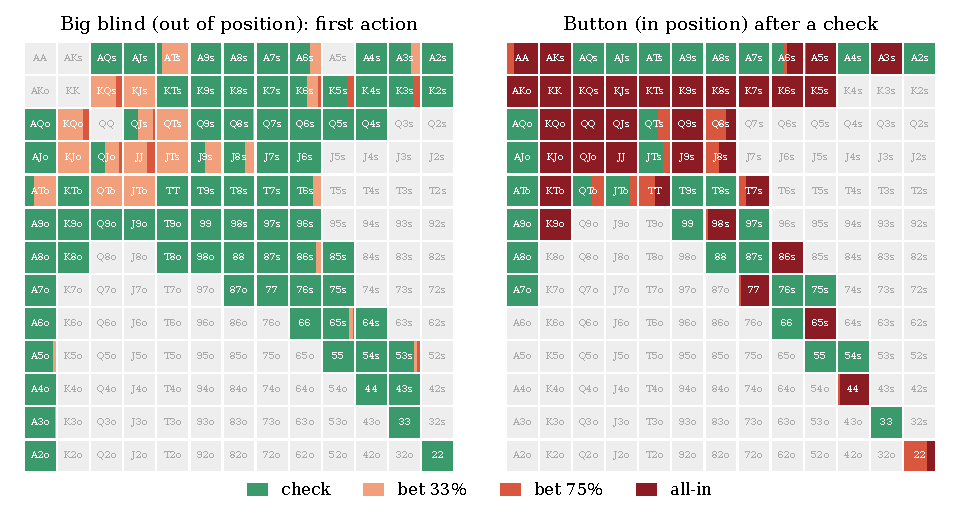
\includegraphics[height=0.6\textheight,trim=0 22 245 0,clip]{grid_root.pdf}\\[-2pt]
{\scriptsize\color{ink2} A solver's answer, computed by our own code. Each square is a starting hand and the colours are actions.}
\end{columns}
\note{
The common core of all these programs is an iterative method, counterfactual regret minimisation, applied to a very large
saddle-point problem. Libratus and DeepStack add abstraction (shrinking the game) and subgame solving
(solving again the part of the game you are actually in), but the inner loop is still a method of the CFR family.\\[3pt]
Commercial solvers such as PioSolver, GTO+ and GTO Wizard are what human players use. You give the board, the
two ranges and the allowed bet sizes, and the program computes an equilibrium of that subgame. The picture on the right is
exactly such an output, produced by our solver for the river situation that we use for the whole talk.\\[3pt]
References if asked: Bowling et al., Science 2015. Morav\v{c}\'ik et al., Science 2017. Brown and Sandholm, Science 2018 and 2019.
}
\end{frame}

% =====================================================================================
\begin{frame}{The plan: poker $\leftrightarrow$ math}
\centering
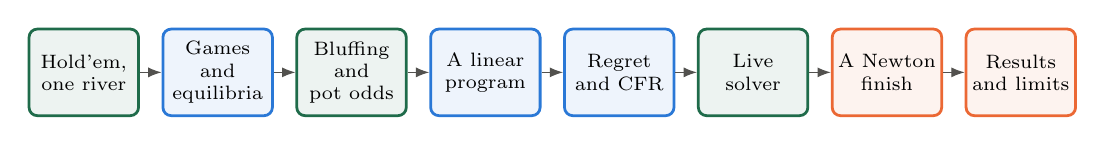
\begin{tikzpicture}[x=1cm,y=1cm,every node/.style={font=\scriptsize}]
  \foreach \i/\t/\c in {0/{Hold'em,\\ one river}/felt, 1/{Games and\\ equilibria}/cblue, 2/{Bluffing and\\ pot odds}/felt,
                       3/{A linear\\ program}/cblue, 4/{Regret\\ and CFR}/cblue, 5/{Live\\ solver}/felt,
                       6/{A Newton\\ finish}/corange, 7/{Results\\ and limits}/corange}{
    \node[draw=\c,line width=1pt,rounded corners=3pt,text width=1.25cm,minimum height=1.1cm,align=center,
          inner sep=2pt,fill=\c!8] (n\i) at (1.7*\i,0) {\t};
  }
  \foreach \i [evaluate=\i as \j using int(\i+1)] in {0,...,6} { \draw[-{Latex},ink2] (n\i) -- (n\j); }
\end{tikzpicture}

\vspace{1.4em}
\raggedright
The equilibrium of a poker game is the solution of a very large and very structured saddle-point problem.
Solvers attack it with a first-order method whose steps are cheap and whose last digits are slow.

\medskip
In the middle of the talk we solve a real hand live in the browser and look at the answer together.

\medskip
Our own contribution comes last. We treat the end of the solve as a nonsmooth equation and finish it with a Newton
method, which reaches machine precision where the first-order method would need millions of iterations.
\note{
Say what the audience will get. First, enough poker to read the output of a solver. Second, the mathematics of why CFR converges
and why it is fast in practice. Third, a live demonstration in which they can ask for any change to the hand. Fourth, a new method
from the numerical optimisation toolbox, with honest results: where it wins by orders of magnitude, and where it does not yet.
}
\end{frame}

% =====================================================================================
\begin{frame}{\tagP\ Texas hold'em in one slide}
\begin{columns}[T]
\column{0.5\textwidth}
Each of the two players is dealt two private cards. Five public cards, the \emph{board}, are then revealed in three
stages called the flop, the turn and the river.

\medskip
There is a round of betting before the flop and after each stage. A player may check, bet, call, raise or fold, and in the
no-limit game a bet can be any size up to the player's stack.

\medskip
If nobody folds, the best five-card hand made from the seven available cards wins the pot.
\column{0.48\textwidth}
\centering
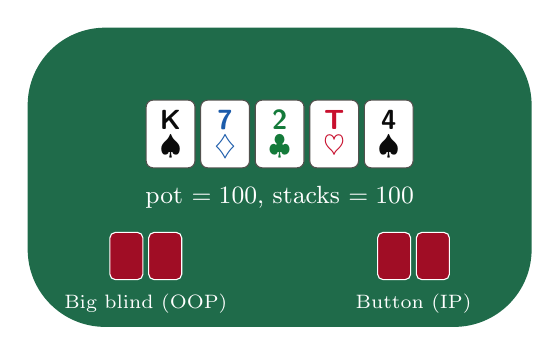
\begin{tikzpicture}
  \fill[felt,rounded corners=28pt] (-3.2,-1.9) rectangle (3.2,1.9);
  \node at (0,0.55) {\pcard{K}{s}\,\pcard{7}{d}\,\pcard{2}{c}\,\pcard{T}{h}\,\pcard{4}{s}};
  \node[text=white,font=\small] at (0,-0.25) {pot $= 100$, stacks $= 100$};
  \node at (-1.7,-1.0) {\cardback\,\cardback};
  \node at (1.7,-1.0) {\cardback\,\cardback};
  \node[text=white,font=\scriptsize] at (-1.7,-1.6) {Big blind (OOP)};
  \node[text=white,font=\scriptsize] at (1.7,-1.6) {Button (IP)};
\end{tikzpicture}\\[4pt]
{\small Our running example is the \alert{river}, the last round of betting.\\
The big blind acts first, which is called being out of position.}
\end{columns}
\note{
Keep this light, since most of the audience has played or watched poker. The key structural fact is that the board is
public and the two hole cards are private. A strategy must therefore be a function of
the public history and your own cards. You do not know the opponent's cards, only a probability distribution over them,
which poker players call a \textbf{range}.\\[3pt]
The river situation is fixed for the whole talk: board K$\spadesuit$ 7$\diamondsuit$ 2$\clubsuit$ T$\heartsuit$ 4$\spadesuit$, pot 100, both players
have 100 behind. The big blind may check or bet 33\% or 75\% of the pot or go all-in. Facing a bet you may fold, call or go all-in.
The live demonstration uses exactly this table.
}
\end{frame}

% =====================================================================================
\begin{frame}{\tagP\ Ranges: what a solver takes as input}
\begin{columns}[T]
\column{0.6\textwidth}
\centering
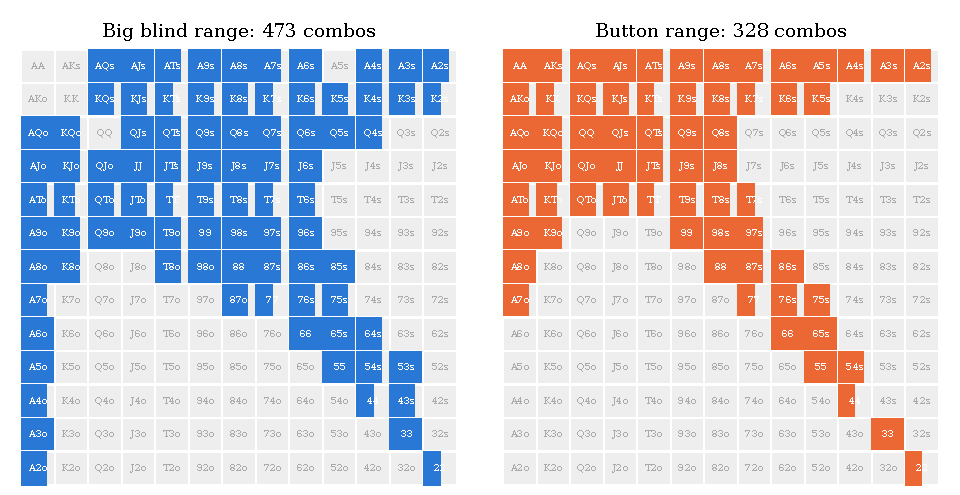
\includegraphics[width=\linewidth]{ranges.pdf}
\column{0.38\textwidth}
A \textbf{range} is a probability vector over the two-card hands a player can hold. There are 1326 such hands, and 1081
once the five board cards are known.

\medskip
In our example the big blind called a raise before the flop and the button made that raise, so the two ranges are
different.

\medskip
The solver returns, for every point of the betting and for every hand, a probability for each action.
\end{columns}
\note{
The 13 by 13 grid is the standard poker picture. Pairs are on the diagonal, suited hands above it and offsuit hands below it.
Each cell is a class of hands, for example AKs stands for 4 combinations. Mathematically the input is two nonnegative vectors
$r_1\in\R^{n_1}$ and $r_2\in\R^{n_2}$. Two hands that share a card cannot both be dealt, which is called card removal, and it is a 0/1
compatibility matrix $C$ between the ranges. Both will appear in the formulas later.\\[3pt]
The width of each bar shows how many combinations are still possible given the board. The king of spades is on the board, so there
are fewer hands with a king.
}
\end{frame}

% =====================================================================================
\begin{frame}{\tagM\ Two-player zero-sum games and Nash equilibrium}
Each player chooses a strategy from a compact convex set, $x\in X$ and $y\in Y$, and the first player receives the
bilinear payoff $x^\top A y$ from the second.
\begin{block}{Minimax theorem (von Neumann 1928)}
\[ \max_{x\in X}\min_{y\in Y} x^\top A y \;=\; \min_{y\in Y}\max_{x\in X} x^\top A y \;=:\; v^\ast . \]
\end{block}
A pair $(x^\ast,y^\ast)$ that attains both sides is a \textbf{Nash equilibrium}, and $v^\ast$ is the value of the game.
Playing $x^\ast$ guarantees at least $v^\ast$ against any opponent, which is what poker players mean by an unexploitable strategy.
\begin{block}{The error that every solver reports is the exploitability}
\[\ex(x,y) \;=\; \tfrac12\Big(\max_{x'} x'^\top A y \;-\; \min_{y'} x^\top A y'\Big)\;\ge 0 ,
  \qquad\text{with equality exactly at an equilibrium.}\]
\end{block}
\note{
For an applied mathematics audience this is a convex-concave saddle-point problem with a bilinear coupling, and the exploitability
is the primal-dual gap. Everything later is a method for driving this gap to zero. Its unit is chips per hand.\\[3pt]
Practical solvers stop at an exploitability of a fraction of a percent of the pot. We will push to $10^{-13}$.
Our numbers are in chips with a pot of 100, so $10^{-2}$ chips is $10^{-4}$ of the pot.
}
\end{frame}

% =====================================================================================
\begin{frame}{\tagP\ Why equilibria mix: bluffing and pot odds}
\begin{columns}[T]
\column{0.56\textwidth}
Take a toy river with a pot of 1. The bettor holds either the best hand or nothing and bets $s$. The caller holds a
medium hand that only beats a bluff.

\medskip
The caller is indifferent between calling and folding when bluffs are a fraction $\beta = \dfrac{s}{1+2s}$ of the bets.

\medskip
The bettor's bluffs are indifferent when the caller continues with probability $\dfrac{1}{1+s}$. Poker players call
this the \emph{minimum defence frequency}.

\medskip
Any pure strategy can be exploited here. The equilibrium randomises, and it does so exactly where the opponent
is made indifferent.
\column{0.4\textwidth}
\centering
\begin{tabular}{ccc}
\toprule
bet $s$ & bluffs $\beta$ & defend \\ \midrule
$1/3$ & 20\% & 75\% \\
$3/4$ & 30\% & 57\% \\
$1$ & 33\% & 50\% \\
$2$ & 40\% & 33\% \\ \bottomrule
\end{tabular}\\[10pt]
{\small We will check the last column against the live solver.}
\end{columns}
\note{
Derivation, to say and not to write. For the caller, calling wins $1+s$ against a bluff and loses $s$ against a value bet.
The caller is indifferent when $\beta(1+s) = (1-\beta)s$, which gives $\beta = s/(1+2s)$. For the bettor with nothing, betting wins the pot $1$
when the caller folds and loses $s$ when called, and checking wins nothing. The bettor is indifferent when $(1-c)\cdot 1 = c\, s$, which gives $c = 1/(1+s)$.\\[3pt]
The mathematical point: at an equilibrium every action played with positive probability is a best response. This is
complementary slackness in the linear program that we are about to write down. Mixing happens exactly where reduced costs vanish.
}
\end{frame}

% =====================================================================================
\begin{frame}{\tagM\ Games on trees with hidden information}
\begin{columns}[T]
\column{0.52\textwidth}
Poker is a game tree. Chance deals the cards, the players act in turn, and the leaves carry the payoffs.

\medskip
A player cannot see the opponent's cards, so several nodes look the same to that player. Such a group of
nodes is an \textbf{information set}, and a strategy assigns a probability distribution over actions to each one.

\medskip
{\footnotesize
\begin{tabular}{lr}
\toprule
game & information sets \\ \midrule
Kuhn poker & 12 \\
Leduc hold'em & 288 \\
Limit hold'em & $3.2\times10^{14}$ \\
No-limit hold'em & about $10^{161}$ \\ \bottomrule
\end{tabular}}
\column{0.46\textwidth}
\centering
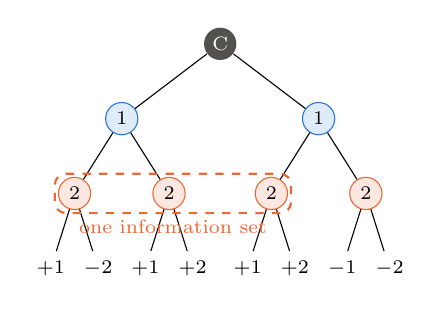
\begin{tikzpicture}[level distance=0.95cm,
   level 1/.style={sibling distance=2.5cm},level 2/.style={sibling distance=1.2cm},level 3/.style={sibling distance=0.6cm},
   every node/.style={font=\scriptsize}]
  \node[circle,fill=ink2,text=white,inner sep=1.5pt] {C}
    child { node[circle,draw=cblue,fill=cblue!15,inner sep=2pt] (a) {1}
       child { node[circle,draw=corange,fill=corange!15,inner sep=2pt] (b1) {2} child{node{$+1$}} child{node{$-2$}} }
       child { node[circle,draw=corange,fill=corange!15,inner sep=2pt] (b2) {2} child{node{$+1$}} child{node{$+2$}} } }
    child { node[circle,draw=cblue,fill=cblue!15,inner sep=2pt] (c) {1}
       child { node[circle,draw=corange,fill=corange!15,inner sep=2pt] (d1) {2} child{node{$+1$}} child{node{$+2$}} }
       child { node[circle,draw=corange,fill=corange!15,inner sep=2pt] (d2) {2} child{node{$-1$}} child{node{$-2$}} } };
  \draw[corange,dashed,thick,rounded corners] ($(b1)+(-0.25,0.25)$) -- ($(d1)+(0.25,0.25)$) -- ($(d1)+(0.25,-0.25)$) -- ($(b1)+(-0.25,-0.25)$) -- cycle;
  \node[corange,font=\scriptsize] at ($(b1)!0.5!(d1)+(0,-0.42)$) {one information set};
\end{tikzpicture}\\[2pt]
{\scriptsize Player 2 sees the action of player 1 but not the deal.}
\end{columns}
\note{
Leduc hold'em is the standard research benchmark. It has a deck of six cards, one private
card each, one public card, and two betting rounds. It has 288 information sets and we use it as our small test problem.\\[3pt]
The size column is the reason the subject exists. Nobody can write down no-limit hold'em. Real systems solve an abstraction
in which similar hands and bet sizes are merged, and then solve subgames like our river again during play.\\[3pt]
We assume perfect recall: a player never forgets what he knew or did. Sizes are from Bowling et al.\ 2015 and Johanson 2013.
Kuhn and Leduc were counted by our code.
}
\end{frame}

% =====================================================================================
\begin{frame}{\tagM\ The sequence form: equilibrium is a linear program}
Give player 1 one variable $x_\sigma$ for each \emph{sequence} $\sigma$ of her own
actions, equal to the product of her probabilities along it. These variables satisfy linear flow constraints
$Ex = e$, $x\ge 0$, and the expected payoff is bilinear in them, $u(x,y) = x^\top A y$.
\begin{block}{Theorem (Koller, Megiddo and von Stengel 1996)}
An equilibrium strategy of player 1 solves
\[\max_{x,\,q}\ f^\top q\quad \text{subject to}\quad A^\top x - F^\top q \ge 0,\quad Ex = e,\quad x\ge 0 ,\]
a linear program whose size is \emph{linear} in the size of the game tree.
\end{block}
So why not call an LP solver? On our river $A$ has 2.9 million nonzeros, because every leaf couples every hand of one
player to every hand of the other, and a good LP code did not finish in 25 minutes. The iteration we describe next
reaches $\MedDCFRExpl$ chips in \MedDCFRTime\ seconds.
\note{
This is the key modelling step. Mixed strategies over the pure strategies of the normal form would have exponentially many
variables. Realisation plans have one variable per sequence, and perfect recall makes the payoff bilinear in them.\\[3pt]
$E$ and $F$ are very sparse, with one row per information set and entries $\pm1$, and they encode flow conservation on a tree.
$A$ is where the poker lives. The program has 17{,}626 unknowns on our river. Say that the dual variables $q$ are the values of the opponent's information sets, and remember them: they are values of information sets, the same quantities
that CFR computes in every iteration. This is how we will warm-start the duals later.\\[3pt]
The LP run used HiGHS through SciPy with default settings on one core and we stopped it after 25 minutes. On the smaller test
problems the LP is perfectly fine: 0.04 s on Leduc and 1.6 s on a small river. The DCFR figure is for \MedDCFRIters\ iterations.
}
\end{frame}

% =====================================================================================
\begin{frame}{\tagM\ Regret matching}
\begin{columns}[T]
\column{0.62\textwidth}
We face the same decision many times. The \emph{regret} $R_T(a)$ of an action is how much better it would have done
than what we played. Regret matching plays each action in proportion to its positive regret.
{\small\[ R_T(a) = \sum_{t=1}^T \big(u_t(a) - u_t(\sigma_t)\big),\quad
   \sigma_{T+1}(a) = \frac{[R_T(a)]^+}{\sum_b [R_T(b)]^+}. \]}
\begin{block}{Theorem (Hart and Mas-Colell 2000)}
The regrets grow only like $\sqrt{T}$: $\ \max_a R_T(a) \le \Delta\sqrt{|A|\,T}$.
\end{block}
When both players of a zero-sum game do this, their \emph{average} strategies converge to an equilibrium.
\column{0.36\textwidth}
\centering
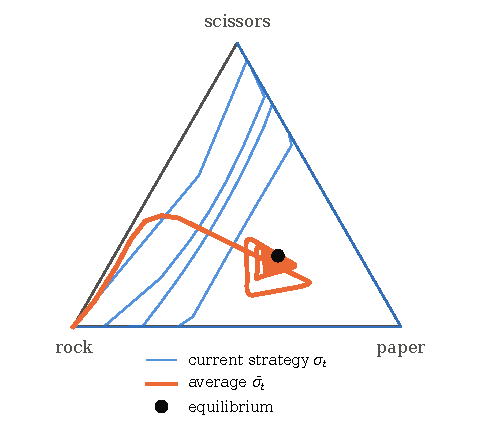
\includegraphics[width=\linewidth]{rm_rps.pdf}\\
{\scriptsize Our computation on a weighted rock-paper-scissors game. The current strategy cycles and the average converges.}
\end{columns}
\note{
Idea of the proof. The regret vector satisfies $\|[R_{T}]^+\|^2 \le \|[R_{T-1}]^+\|^2 + \Delta^2|A|$ because the
cross term $\langle [R_{T-1}]^+, r_T\rangle$ vanishes by the choice of $\sigma_T$: the instantaneous regret is orthogonal to the
current positive regrets. Sum and take square roots. This is Blackwell approachability, and $\Delta$ is the range of the payoffs.\\[3pt]
The folk theorem: if both players have average regret at most $\varepsilon$ then the average strategies are a $2\varepsilon$-equilibrium,
because $\max_{x'} x'^\top A \bar y - \min_{y'} \bar x^\top A y' \le 2\varepsilon$.\\[3pt]
In the figure the limit is $(\frac14,\frac12,\frac14)$.
}
\end{frame}

% =====================================================================================
\begin{frame}{\tagM\ Counterfactual regret minimisation (CFR)}
CFR runs regret matching separately at every information set $I$. The payoff it feeds to each one is the
\textbf{counterfactual value} of an action, which is the expected payoff weighted by the probability that the opponent and
chance lead to $I$, as if the player herself had tried to get there.
\[ v_i(\sigma, I, a) = \sum_{h\in I}\ \pi_{-i}^{\sigma}(h)\sum_{z \sqsupset ha} \pi^{\sigma}(ha\to z)\, u_i(z) \]
\begin{block}{Theorem (Zinkevich, Johanson, Bowling and Piccione 2007)}
The regret of the whole strategy is at most the sum of the local regrets. Therefore the average strategies satisfy
\[ \ex(\bar x_T,\bar y_T) \ \le\ \frac{\Delta\,|\mathcal I|\sqrt{|A|}}{\sqrt T}. \]
\end{block}
One iteration is one pass over the tree, with reach probabilities computed on the way down and values on the way up.
The matrix $A$ is never formed.
\note{
The decomposition is the whole trick. A global regret over an exponentially large strategy space is bounded by a sum of small
local regrets, and each of them is minimised by plain regret matching. This is why CFR scales: the cost of an iteration is linear in the tree
and so is the storage, two numbers for each information set and action.\\[3pt]
In the language of linear algebra, one CFR iteration computes $Ay$ and $A^\top x$ for the current realisation plans by walking the tree.
These are the same two products that any first-order saddle-point method needs.
}
\end{frame}

% =====================================================================================
\begin{frame}{\tagP\tagM\ CFR for poker: one pass for all hands}
In poker the betting is public and only the cards are hidden. At each point of the betting we store
\emph{vectors} indexed by hands, such as the reach probabilities $\pi_1$ and $\pi_2$.
At a leaf the values of all hands come from one matrix-vector product.
\[ v_1 = \text{amount}\cdot B\,\pi_2,\qquad
   B_{ij} = \underbrace{C_{ij}}_{\text{no shared card}}\cdot\begin{cases} 1 & \text{after a fold}\\ \operatorname{sign}(s_i - s_j) & \text{at a showdown}\end{cases} \]
Here $s_i$ is the strength of hand $i$. The matrix $B$ is dense but very structured. Once the hands are sorted by
strength, the sign matrix is all ones below the diagonal and all minus ones above it, and $C$ is the all-ones matrix
minus a sparse correction for hands that share a card.

\medskip
As a result $B\pi$ costs one sort and a running sum, which is $O(n\log n)$ operations and not $n^2$.
\note{
This is the bridge between the tree picture and the implementation. The information sets at a public node are indexed by the
private hand of the player to act, so all information sets at this node form a vector and every CFR operation becomes a vector operation.\\[3pt]
This is also the poker-specific numerical linear algebra. Each terminal block is low rank plus sparse. The fold block is
rank one minus a sparse correction. The showdown block, after sorting, is a sign matrix, which is semiseparable (think of the inverse of
a bidiagonal matrix), times the compatibility mask. The trick is due to Johanson et al.\ 2011.\\[3pt]
The public tree itself is drawn live in the demonstration, so it is not on a slide any more. It has 12 decision points and 21 leaves, and one iteration takes about a millisecond in the browser. Keep in mind that this structure is what a
scalable Newton method would have to exploit, which comes back at the end of the talk.
}
\end{frame}

% =====================================================================================
\begin{frame}{\tagM\ Four variants of one loop}
Modern solvers change how CFR weights the old regrets and how it averages the strategies.

\smallskip
\renewcommand{\arraystretch}{1.15}\small
\begin{tabular}{p{1.5cm}p{6.4cm}p{5.0cm}}
\toprule
method & what changes & a numerical analyst would say \\ \midrule
CFR$^+$ & Negative regrets are reset to zero and later strategies get more weight in the average. & projection onto the nonnegative orthant \\
DCFR & Old regrets and old strategies are multiplied by factors below one. & forgetting factors that damp the transient \\
PCFR$^+$ & The strategy is computed from the regrets plus a prediction of the next regret. & optimism, as in the extragradient method \\ \bottomrule
\end{tabular}

\smallskip
\normalsize The proven rate is still $T^{-1/2}$ for all four. In practice the modern variants are much faster, and we will
now race them against each other on a real hand.
\note{
CFR$^+$ (Tammelin 2014) is what solved limit hold'em. DCFR (Brown and Sandholm 2019) with parameters $(1.5, 0, 2)$ is the default in many solvers:
positive regrets are multiplied by $t^{1.5}/(t^{1.5}+1)$, negative ones by $1/2$, and the average by $(t/(t+1))^2$.
PCFR$^+$ (Farina, Kroer and Sandholm 2021) uses the last instantaneous regret as its prediction and connects regret matching to optimistic mirror descent.\\[3pt]
All four also update the two players in turn, so that the second player already sees the new strategy of the first, which is Gauss-Seidel in place of Jacobi.\\[3pt]
The observed rates are between $T^{-1}$ and $T^{-3/2}$ for the averages, while the last iterate oscillates. Explaining this gap to the
theory is an open question. The rates are still sublinear, and that is the gap our method addresses.
}
\end{frame}

% =====================================================================================
\begin{frame}{\tagP\tagM\ Live demonstration: the river solver table}
\begin{columns}[c]
\column{0.55\textwidth}
\centering
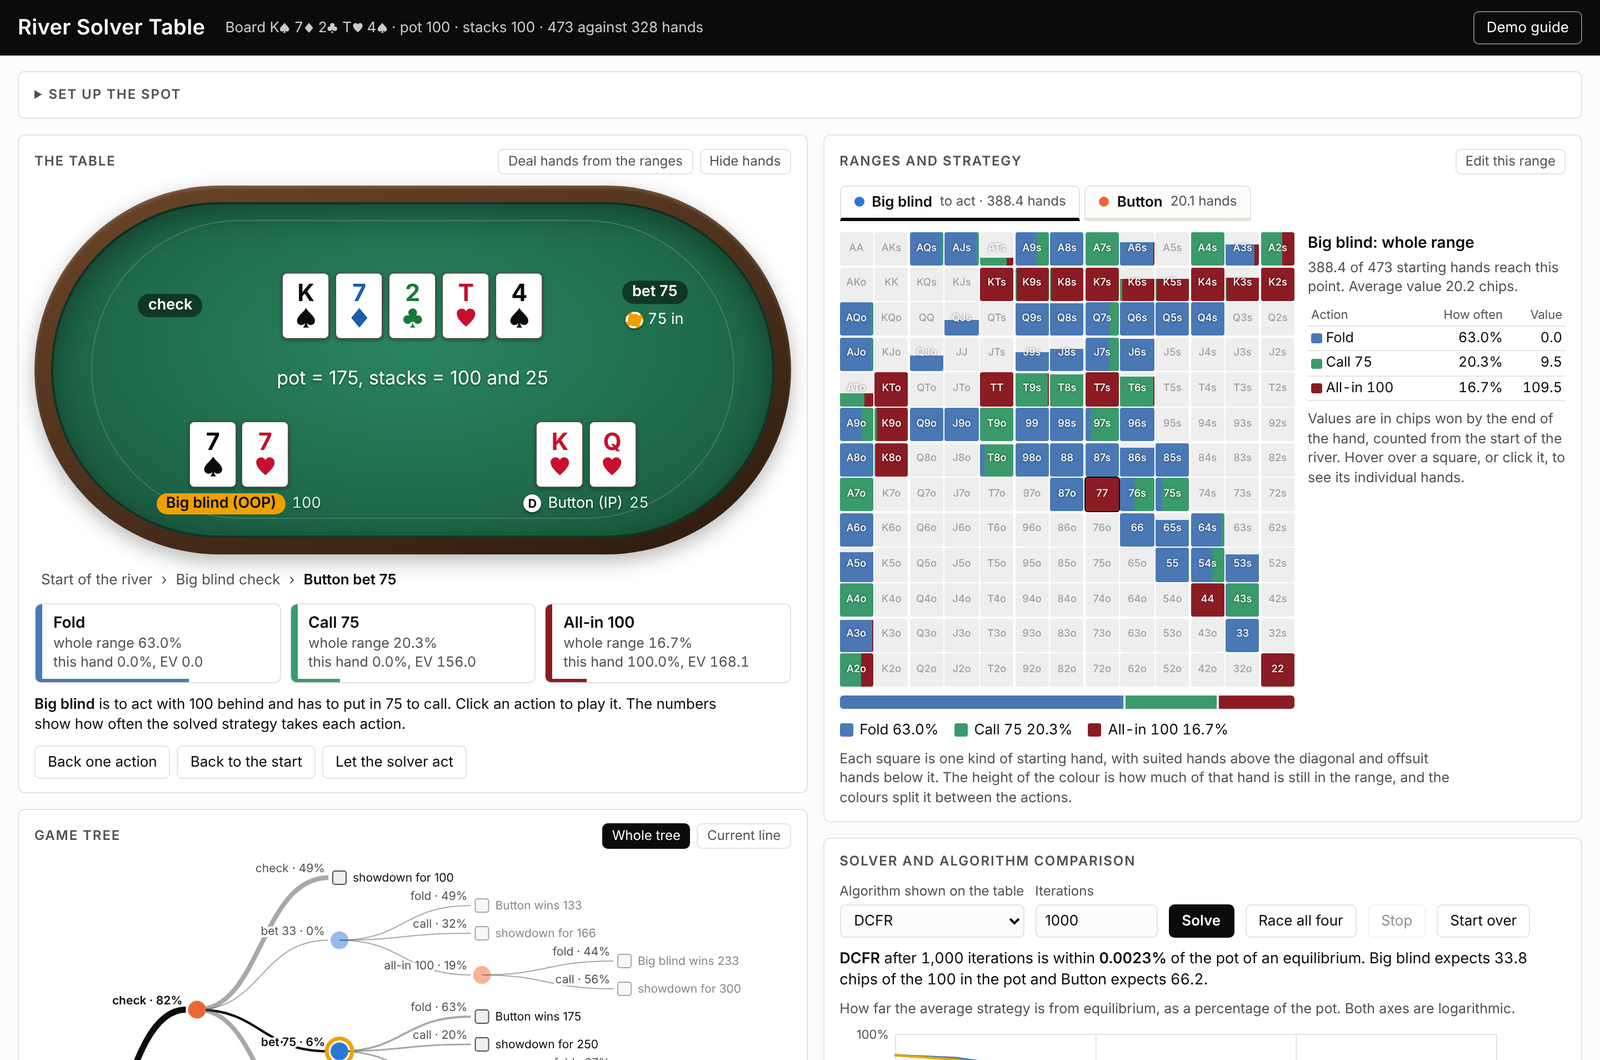
\includegraphics[width=\linewidth]{app_slide.png}
\column{0.43\textwidth}
The page \texttt{app/poker-solver.html} solves our river in the browser. It will answer five questions.
\begin{enumerate}\small\setlength\itemsep{2pt}
\item Which of the four algorithms wins a race?
\item What does the big blind do with each of its 473 hands?
\item How do the ranges and the tree change as the hand is played?
\item Does a hand that mixes get the same value from both actions?
\item Does the solver agree with the pot odds formula?
\end{enumerate}
After that the board, the ranges and the bet sizes are yours to change.
\end{columns}
\note{
Switch to the browser now. The full script with what to click and what to say is in \texttt{app/DEMO\_NOTES.md} (also as a PDF),
and the same steps are in the Demo guide inside the page. Budget twelve minutes.\\[3pt]
Short version of the script. (1) Load the page, which solves the spot with DCFR in two seconds. Point at the table, the grid, the tree and the chart.
(2) Press Race all four. After 1000 iterations CFR is at about 0.11\% of the pot, PCFR$^+$ at 0.009\%, CFR$^+$ at 0.007\% and DCFR at 0.002\%.
(3) Read the big blind's grid: check 82\%, bet a third of the pot 16\%, bet three quarters 2\%. Value bets and bluffs.
(4) Give the big blind three sevens: it checks every time, and after the button bets 75 it raises all-in every time.
(5) After check and bet 75, select ace-nine offsuit: it folds 63\% and calls 37\%, and both actions are worth 0.0 chips.
(6) After the big blind bets 33, the button folds 26\%, and the formula says at most 25\%. After a check and an all-in the big blind folds 68\%, far more than the formula's 50\%.
(7) Change the river card to the nine of hearts and solve again. Then take requests from the audience.\\[3pt]
If the browser fails, the static grids are in \texttt{talk-detailed.pdf}, slides 18 and 19.
}
\end{frame}

% =====================================================================================
\begin{frame}{\tagP\ What the demonstration showed}
\begin{columns}[T]
\column{0.42\textwidth}
The solution reads like poker. Strong hands bet, a few hands with nothing bluff, and the hands in between check.

\medskip
A hand that mixes two actions gets the same value from both. This is complementary slackness.

\medskip
The button defends within 1.5 points of the pot odds formula. The big blind folds much more than the formula says,
because the button's bluffs would still win some showdowns by checking.
\column{0.57\textwidth}
\centering
{\scriptsize\setlength\tabcolsep{3pt}
\begin{tabular}{@{}llccc@{}}
\toprule
defender & line & $s$ & defends & MDF \\ \midrule
Button & BB checks, BTN bets 75, BB jams & $0.10$ & $64.7\%$ & $90.9\%$ \\
Button & BB bets 33 & $0.33$ & $74.3\%$ & $75.2\%$ \\
Button & BB checks, BTN bets 33, BB jams & $0.40$ & $57.8\%$ & $71.2\%$ \\
Button & BB bets 75 & $0.75$ & $55.8\%$ & $57.1\%$ \\
Button & BB bets 100 & $1.00$ & $49.1\%$ & $50.0\%$ \\
Big blind & BB bets 75, BTN jams & $0.10$ & $63.4\%$ & $90.9\%$ \\
Big blind & BB checks, BTN bets 33 & $0.33$ & $52.2\%$ & $75.2\%$ \\
Big blind & BB bets 33, BTN jams & $0.40$ & $56.3\%$ & $71.2\%$ \\
Big blind & BB checks, BTN bets 75 & $0.75$ & $37.5\%$ & $57.1\%$ \\
Big blind & BB checks, BTN bets 100 & $1.00$ & $32.6\%$ & $50.0\%$ \\
\bottomrule
\end{tabular}
}\\[6pt]
{\scriptsize Exact equilibrium of our river. Here $s$ is the bet as a fraction of the pot, MDF is $1/(1+s)$, and a jam is an all-in bet.}
\end{columns}
\note{
This is a consistency check of the whole pipeline. When the big blind bets, the button defends 74.3\% against 75.2\%, 55.8\% against
57.1\% and 49.1\% against 50.0\%, so the toy formula is almost exact. When the button bets after a check, the big blind folds much
more. We checked that the button's weakest betting hands mix between checking and going all-in, so the indifference that fixes
the defence frequency is ``value of the all-in equals value of checking, which is positive'' and not ``value of the all-in equals zero''.\\[3pt]
The numbers in the table come from the exact equilibrium computed by the method of the next part, so they can differ in the last digit from what the
browser showed after 1000 iterations.
}
\end{frame}

% =====================================================================================
\begin{frame}{\tagM\ Why push the precision further?}
\begin{columns}[T]
\column{0.58\textwidth}
Practical solvers stop at about 0.1\% of the pot, and for a human studying a hand that is plenty.

\medskip
More digits matter when a program stitches many small solves together and their errors add up, when we ask exactly which
hands mix, and when research needs a ground truth with a certificate.

\medskip
For a numerical analyst, CFR is a first-order method on a nonsmooth and degenerate problem. It is
robust and cheap, and its tail is sublinear. The classical cure for a slow tail is a \alert{local method of higher
order}, started from a good point.
\column{0.4\textwidth}
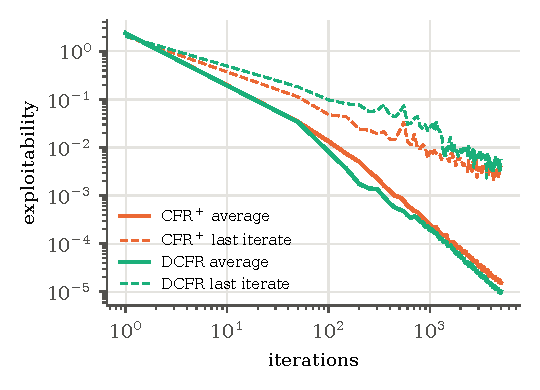
\includegraphics[width=\linewidth]{avg_vs_last.pdf}\\
{\scriptsize Our computation on Leduc. Only the average converges, and each extra digit costs about ten times more iterations.}
\end{columns}
\note{
Make the case without overselling. Precision matters for machines (solving subgames again, evaluation) and for science
(knowing the exact equilibrium, for example the exact bluffing frequencies, or whether a hand mixes at all).\\[3pt]
The analogy for this audience: CFR is like a stationary iterative method. It is fantastic for the first
digits and hopeless for the last ones, and the obvious idea is to switch to a Newton-type method near the solution.\\[3pt]
Numbers for Leduc: CFR$^+$ reaches $\LeducCFRplusLong$ after 50{,}000 iterations and \LeducCFRplusLongTime\ seconds. The curves are on a backup slide.
}
\end{frame}

% =====================================================================================
\begin{frame}{\tagO\ Step 1: write the equilibrium as a variational inequality}
Collect both strategies and both vectors of information-set values in one unknown $z = (x, y, p, q)$. An
equilibrium is a point that satisfies the optimality conditions of both players' linear programs.
\[
\begin{aligned}
 0\le x \ &\perp\ E^\top p - A y \ \ge 0, & Ex &= e,\\
 0\le y \ &\perp\ A^\top x - F^\top q \ \ge 0, & Fy &= f.
\end{aligned}
\]
These conditions have the form $w = Mz + b$ with a matrix that is \textbf{skew-symmetric}.
\[ M = \begin{pmatrix} 0 & -A & E^\top & 0\\ A^\top & 0 & 0 & -F^\top\\ -E & 0 & 0 & 0\\ 0 & F & 0 & 0\end{pmatrix},
   \qquad M + M^\top = 0 . \]
Skew symmetry makes the problem monotone. It also means that the solutions form a polyhedron and
not a single point, so Newton's method cannot be applied directly. CFR gives a starting point for all of $z$ for free.
\note{
This is a mixed linear complementarity problem. The reduced cost $E^\top p - Ay$ of a sequence is its counterfactual
regret scaled by reach, and complementarity says ``play only actions with zero regret''. So CFR and this system talk
about the same quantities: the CFR average strategies are $x$ and $y$, and its best-response values are $p$ and $q$.\\[3pt]
Skewness: the $x$-$y$ block is the zero-sum coupling. The $(x,p)$ and $(y,q)$ blocks are pairs of constraints and multipliers, arranged
with signs so that $M^\top = -M$.\\[3pt]
Non-uniqueness is already visible in Kuhn poker, where the equilibria form a one-parameter family (backup slide).\\[3pt]
If asked what we tried first: Anderson acceleration of the CFR$^+$ map, vector extrapolation of the averages, and Levenberg-Marquardt on the
optimality system. None of them beat DCFR on Leduc. The CFR map is piecewise linear with non-isolated fixed points, and the acceleration theory needs a smooth contraction.
The details are in \texttt{talk-detailed.pdf}.
}
\end{frame}

% =====================================================================================
\begin{frame}{\tagO\ Step 2: the proximal point method makes each problem well posed}
We add a small multiple of the identity. Given $z^k$, the next iterate $z^{k+1}$ solves the same conditions with
\[ w_\rho(z) = (M + \rho I)\,z + b - \rho\, z^{k} . \]
\begin{columns}[T]
\column{0.56\textwidth}
Since $d^\top(M+\rho I)d = \rho\|d\|^2$, the matrix $M+\rho I$ is positive definite and each regularised problem
has exactly one solution.

\medskip
\textbf{Theorem (Rockafellar 1976, Luque 1984).} The iterates converge to a solution of the original problem for every
$\rho>0$. For a polyhedral problem the rate is linear, with a factor that tends to zero with $\rho$.

\medskip
A small $\rho$ gives a fast outer loop and badly conditioned inner problems.
\column{0.41\textwidth}
\begin{block}{Our computation on Leduc with $\rho = 10^{-5}$}
\small The residual after each outer step:\\[2pt]
$3.4\!\times\!10^{-2} \to 4.8\!\times\!10^{-6} \to 3.3\!\times\!10^{-9}$\\ $\to 6.9\!\times\!10^{-12} \to 2.0\!\times\!10^{-14}$\\[3pt]
About three digits for each step.
\end{block}
\end{columns}
\note{
The proximal term fixes the non-uniqueness. Each subproblem has exactly one solution, so Newton's method has a well defined and
nonsingular target. For polyhedral monotone problems the inverse operator is upper Lipschitz (Robinson 1981), which gives linear
convergence of the proximal point method with a factor that tends to zero as $\rho\to0$.\\[3pt]
The trade-off is the whole story of the last part of the talk. A small $\rho$ makes the outer loop fast and the inner problems
nearly as ill posed as the original one, since $\|(M+\rho I)^{-1}\|\le 1/\rho$. There is a backup slide with the rate.
}
\end{frame}

% =====================================================================================
\begin{frame}{\tagO\ Step 3: Newton's method on a piecewise-linear equation}
Each regularised problem can be written as one equation. For every action, either its probability is zero or its
reduced cost is zero, and that is the same as $\min\big(x_i,\ w_\rho(z)_i\big)=0$.

\medskip
A Newton step for this equation guesses which actions are dropped, imposes indifference on all the others, and solves
one linear system. Its matrix has the form $V = D_a + D_b(M+\rho I)$ with nonnegative diagonal matrices $D_a$ and $D_b$.
\begin{block}{Lemma. Every such $V$ with $D_a+D_b$ positive definite is nonsingular.}
\small Suppose $Vd=0$ and put $u = (M+\rho I)d$. Row $i$ reads $(D_a)_{ii}d_i + (D_b)_{ii}u_i = 0$ with nonnegative coefficients
that are not both zero, so $d_i u_i \le 0$. Hence $\rho\|d\|^2 = d^\top u = \sum_i d_i u_i \le 0$, and $d=0$. \hfill$\square$
\end{block}
If the guess of the dropped actions is right, a single step gives the \emph{exact} solution. If it is wrong there is no
global guarantee, so the method needs a good starting guess.
\note{
The min-function turns complementarity into a piecewise-linear equation. Semismooth Newton on it is exactly the
primal-dual active-set method (Hinterm\"uller, Ito and Kunisch 2002). The lemma is the reason
for the proximal term: without $\rho$ we have $d^\top M d = 0$ and the argument fails. Newton matrices of the unregularised problem
are singular at degenerate solutions, which is what we saw with Levenberg-Marquardt.\\[3pt]
The lemma also covers the Fischer-Burmeister reformulation, which has a smooth merit function and a globally convergent damped Newton method.
We tried it first. It worked on Leduc and on a small river with 50 to 70 linear solves, but on the river of the demonstration it
took steps of size $10^{-3}$ for dozens of iterations. That pushed us to the interior-point start on the next slide.
}
\end{frame}

% =====================================================================================
\begin{frame}{\tagO\ Step 4: making it robust and fast}
\begin{columns}[T]
\column{0.55\textwidth}
\textbf{A robust start.} The first regularised problem is the hardest. We solve it with an interior-point method
started at the CFR point. Its solution tells us which actions are dropped, and from there the Newton steps land
exactly on the solution. Every later problem needs only one to three linear solves.

\medskip
\textbf{Fast linear algebra.} After a change of signs in half of the rows, every linear system is symmetric and
\emph{quasi-definite}. By a theorem of Vanderbei, such a matrix has an $LDL^\top$ factorisation for every ordering of
the unknowns, so we can order for sparsity alone and never pivot.
\column{0.42\textwidth}
\begin{block}{One factorisation, in seconds}
\footnotesize
\begin{tabular}{@{}l@{\ \ }c@{\ \ }c@{}}
& small river & our river\\ \midrule
general sparse LU & 0.11 & 25\\
quasi-definite $LDL^\top$ & 0.04 & 7.6
\end{tabular}
\end{block}
\vspace{4pt}
{\small The whole solve from the CFR point to a residual of $10^{-13}$ takes \LeducSolves\ linear solves on Leduc and
\SmallSolves\ on the small river.}
\end{columns}
\note{
The first problem is the hardest because many actions enter or leave the support. The division of labour mirrors what commercial LP solvers do, interior point and then crossover to a vertex, but inside a proximal
loop and with a game-theoretic warm start. We use Mehrotra's predictor-corrector method. In our runs the interior-point phase took 6 to 8 factorisations on Leduc and the small
river, the crossover a few active-set steps, and every later proximal step 1 to 3 steps. We use $\rho=10^{-5}$ throughout.\\[3pt]
Quasi-definite means the block form $\begin{psmallmatrix} P & B\\ B^\top & -N\end{psmallmatrix}$ with $P$ and $N$ positive definite, after grouping $(x,q)$ and $(y,p)$.
Vanderbei's theorem (1995) lets us choose a fill-reducing ordering before seeing the numbers, which is the same reason interior-point
codes like quasi-definite systems. The timings compare SuperLU with QDLDL on one core.\\[3pt]
A caveat: with only $\pm10^{-5}$ on the diagonal, as in the pure active-set systems, static pivoting is too unstable. There we use a
pivoted sparse LU, which is cheap because the active-set system lives on the support only.
}
\end{frame}

% =====================================================================================
\begin{frame}{\tagP\tagO\ Step 5: restrict to the support, solve exactly, then verify}
\begin{columns}[T]
\column{0.54\textwidth}
On larger hands the method so far fails. Many actions are never played and many positions are never
reached, and in those directions the set of equilibria is \emph{flat}. A point with a tiny residual can be far
from a solution, and the Newton step guesses the wrong dropped actions.

\medskip
The cure is to remove those directions. We keep only the actions that DCFR plays with probability above $10^{-3}$ and
solve this smaller problem exactly.

\medskip
Then we check the answer in the full game. If a removed action would have been profitable we put it back and solve again.
\column{0.43\textwidth}
\begin{block}{The complete method}
\small
\begin{enumerate}\setlength\itemsep{2pt}
\item DCFR for a few thousand iterations
\item keep the actions that it uses
\item solve the restricted problem to machine precision
\item compute exact best responses in the full game
\item add back any profitable action and return to 3
\end{enumerate}
\end{block}
{\small Step 4 is a certificate. The final exploitability is measured in the full game and not assumed.}
\end{columns}
\note{
The verification loop is column generation, the same idea as the double-oracle algorithms for games (McMahan, Gordon and Blum 2003,
Bo\v{s}ansk\'y et al.\ 2014). We also keep only the positions that both players can still reach with the kept actions. What is new is the combination with a support predicted by CFR and an exact
second-order solve of the restricted problem.\\[3pt]
Poker helps here. Equilibria are mostly pure, because mixing happens only at indifference. In the exact Leduc equilibrium about half of the
reachable pairs of information set and hand play a single action, and on the small river 71\%. About half of all sequences are outside the
support, and the dense payoff blocks shrink to the hands that actually reach each leaf.\\[3pt]
On our problems Leduc needed 2 rounds, the small river 1, and the river of the demonstration 3, with 16 actions added back in total. The restricted
problem had about 35\% of the unknowns of the full one.
}
\end{frame}

% =====================================================================================
\begin{frame}{\tagO\ Result on the benchmark game, Leduc hold'em}
\begin{columns}[c]
\column{0.6\textwidth}
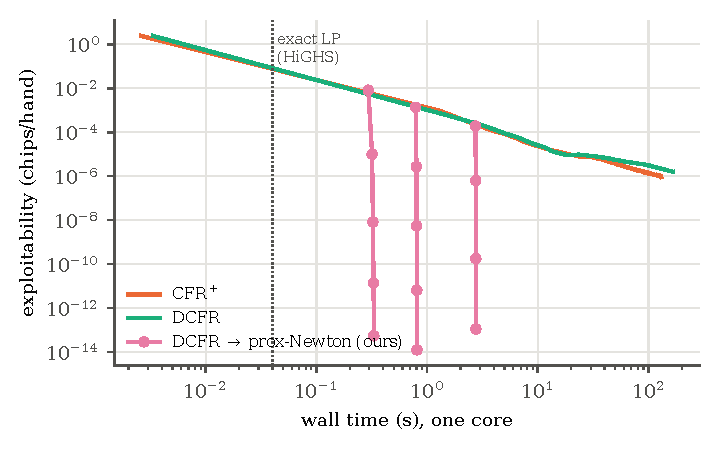
\includegraphics[width=\linewidth]{hybrid_leduc.pdf}
\column{0.38\textwidth}
Each pink curve starts where a short DCFR run stopped and drops straight down to machine precision.

\medskip
From \SuppLeducWarm\ DCFR iterations our method reaches $\SuppLeducExpl$ in \alert{\SuppLeducTime\
seconds}. CFR$^+$ is at $\LeducCFRplusLong$ after \LeducCFRplusLongTime\ seconds.

\medskip
Leduc is tiny and an LP solver needs 0.04 seconds. What matters is the shape of the curves.
\end{columns}
\note{
Each pink curve starts where the DCFR warm start stopped, after 100, 300 or 1000 iterations. The points are verification rounds.
Starting from 100 DCFR iterations is enough and costs one extra round. Starting later only costs DCFR time. The run used \SuppLeducRounds\ rounds and \SuppLeducSolves\ linear solves.\\[3pt]
The value of the game that we obtain, $-0.085606424078\ldots$ chips for the first player, agrees with the LP in all printed digits.\\[3pt]
Be upfront about the LP. Leduc has 964 unknowns and a simplex method finishes in 40 ms. The question is what happens when
the LP does not fit, which is the next slide.
}
\end{frame}

% =====================================================================================
\begin{frame}{\tagO\ Result on the river from the demonstration}
\begin{columns}[T]
\column{0.52\textwidth}
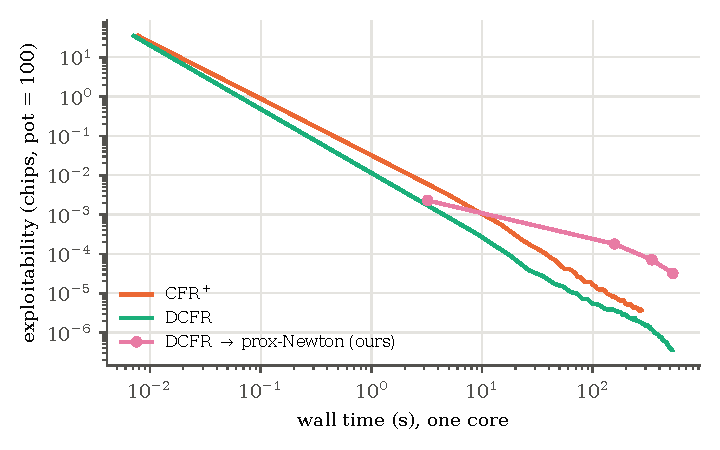
\includegraphics[width=\linewidth]{hybrid_medium.pdf}\\
{\scriptsize 473 against 328 hands and 17{,}626 unknowns. The points are verification rounds.}
\column{0.46\textwidth}
Our method runs DCFR for \SuppMedWarm\ iterations and then needs \SuppMedRounds\ rounds on a problem with \SuppMedFrac\%
of the unknowns. It reaches \alert{$\SuppMedExpl$ chips in \SuppMedTime\ seconds}.

\medskip
At that moment DCFR alone is at $\MedDCFRAtSuppTime$, and after \MedDCFRLongTwoIters\ iterations and \MedDCFRLongTwoTime\
seconds it is at $\MedDCFRLongTwoExpl$.

\medskip
Without the restriction to the support the Newton finish \emph{loses} to DCFR on this hand. The LP solver did not finish in 25
minutes.
\end{columns}
\note{
This is the slide that took the longest to earn. The first version of the method, Newton on the full sequence-form problem, worked
on Leduc and the small river and lost to DCFR here, with $\MedHybExpl$ after \MedHybTime\ seconds. The crossover from the interior point kept landing on a wrong active set,
because the equilibrium set is flat in directions that do not matter, and with
$\rho=10^{-5}$ an error in those directions is amplified by $1/\rho$. A larger $\rho$ made the active-set steps work and the
outer loop crawl. Anderson acceleration of the proximal map helped, to $8\times10^{-7}$ in 8 minutes, and then stalled.\\[3pt]
Restricting to the support predicted by CFR and verifying afterwards removes exactly those directions. \SuppMedAdded\ actions were added back in total.
Starting from 1{,}000 DCFR iterations gives $\SuppMedOneKExpl$ in \SuppMedOneKTime\ seconds.\\[3pt]
On the small river (147 against 139 hands) the method reaches $\SuppSmallExpl$ in \SuppSmallTime\ seconds, DCFR is at $\SmallDCFRExpl$ after \SmallDCFRTime\ seconds, and the LP takes 1.6 seconds. This is on a backup slide.
}
\end{frame}

% =====================================================================================
\begin{frame}{\tagO\ Where it stops winning, and what is open}
\begin{block}{Full ranges: all 1{,}081 hands for both players, 47{,}568 unknowns}
\small The restricted problem still has 43\% of the unknowns and one factorisation takes about 10 seconds. After 80 minutes our
method is at $4.1\times10^{-6}$ chips. DCFR reaches $9.5\times10^{-6}$ in 10 minutes. \textbf{Here CFR wins.}
\end{block}

\medskip
The bottleneck is the linear algebra. Each payoff block is dense, but it is a sorted sign matrix plus a sparse correction,
and a product with it costs $O(n\log n)$. A Newton--Krylov step would then cost only a few CFR iterations, provided we can
find a good preconditioner for systems of the form ``diagonal plus skew''. We think this is the most promising open problem,
and it is a problem in numerical linear algebra.

\medskip
Two further directions are a better prediction of the support from the CFR regrets, which would save verification rounds,
and the use of exact solves inside programs that play in real time.
\note{
The run with full ranges is the honest boundary of the method as implemented. The restriction still removes more than half of the
unknowns, but each factorisation of the remaining system with 20{,}000 unknowns takes about 10 seconds because the payoff blocks between
the hands that remain in play are dense. The first round needed 201 solves and 50 minutes, the second 116, and the second did not
reach machine precision (the proximal loop stalled at a residual of $5\times10^{-7}$).
DCFR does 40{,}000 iterations in 10 minutes.\\[3pt]
The research directions are natural ones for this club. The first is the one I would bet on: the structure that
makes CFR fast (sorting, running sums, card-removal corrections) is exactly the structure that a fast direct or preconditioned iterative
solver for the Newton systems would need. Hierarchical factorisations of the blocks are a candidate.
}
\end{frame}

% =====================================================================================
\begin{frame}{\tagO\ What is new here, and what is not}
The ingredients are classical: the sequence form, the proximal point method, semismooth Newton,
interior point with crossover, quasi-definite factorisations and the CFR family.

\medskip
The closest work is by Yang, Gao, Lin and Kroer (2025), who use a semismooth Newton method for \emph{matrix} games after a
first-order warm start.

\medskip
What we add is a second-order finish that works directly on the sequence form of a poker game. It has four parts:
\begin{itemize}\setlength\itemsep{0pt}
\item the skew formulation with a proximal term, which gives nonsingular Newton matrices by a one-line proof,
\item a warm start for both the strategies and the values taken from CFR,
\item the restriction to the support predicted by CFR, which removes the flat directions,
\item and the verification by exact best responses in the full game.
\end{itemize}
\note{
Be precise about novelty. The general idea of a first-order warm start followed by semismooth Newton for zero-sum games was proposed
for matrix games by Yang, Gao, Lin and Kroer in December 2025 (arXiv 2512.12910). Their Newton system lives on the normal form, they use
Douglas-Rachford splitting and a PRM$^+$ warm start, and they do not treat the structure of extensive-form games.\\[3pt]
To our knowledge no solver based on CFR hands over to a second-order method for the last digits. Early work solved small abstracted games exactly as linear programs (Gilpin and Sandholm 2005). The commercial and research poker solvers that we know of
(PioSolver, GTO+, Libratus, DeepStack) are first-order.
}
\end{frame}

% =====================================================================================
\begin{frame}{Takeaways}
A poker equilibrium is the solution of a structured saddle-point problem, and the sequence form turns it into a linear program
whose size is linear in the game tree.

\medskip
CFR is regret matching at every information set. It never forms the matrix, its proven rate is $T^{-1/2}$, and its modern
variants are much faster in practice, as the race in the browser showed.

\medskip
The output is readable poker: value bets, bluffs, traps and a defence that follows the pot odds.

\medskip
Read as a skew variational inequality, the same problem can be finished by a proximal Newton method. The obstacle is the
flatness of the equilibrium set, and restricting to the support that CFR predicts removes it. On our river this gives
an exploitability of $10^{-12}$ in about two minutes, where DCFR alone is at $10^{-6}$. With full ranges the linear algebra becomes the
bottleneck and CFR wins again.

\medskip
{\small The solver, the interactive page, the benchmarks and these slides are at \texttt{github.com/dwangnumbers/Poker-Solver}.}
\note{
End with the invitation. The open problem on the earlier slide is a natural one for this club: a preconditioner for
shifted skew systems whose off-diagonal blocks are a sorted sign matrix plus a sparse correction.\\[3pt]
If there is time left, go back to the browser and take requests: another board, another range, other bet sizes.
}
\end{frame}

% =====================================================================================
\begin{frame}{Main references}
\footnotesize
\begin{itemize}\setlength\itemsep{1pt}
\item D.~Koller, N.~Megiddo, B.~von Stengel. Efficient computation of equilibria for extensive two-person games. \emph{Games Econ.\ Behav.} 14 (1996).
\item M.~Zinkevich, M.~Johanson, M.~Bowling, C.~Piccione. Regret minimization in games with incomplete information. \emph{NeurIPS} 2007.
\item N.~Brown, T.~Sandholm. Solving imperfect-information games via discounted regret minimization. \emph{AAAI} 2019.
\item R.~T. Rockafellar. Monotone operators and the proximal point algorithm. \emph{SIAM J.\ Control Optim.} 14 (1976).
\item M.~Hinterm\"uller, K.~Ito, K.~Kunisch. The primal-dual active set strategy as a semismooth Newton method. \emph{SIAM J.\ Optim.} 13 (2002).
\item R.~J. Vanderbei. Symmetric quasidefinite matrices. \emph{SIAM J.\ Optim.} 5 (1995).
\item D.~Yang, Y.~Gao, T.~Lin, C.~Kroer. A direct second-order method for solving two-player zero-sum games. arXiv:2512.12910 (2025).
\end{itemize}
The complete list of references is in \texttt{talk-detailed.pdf}.
\end{frame}

% =====================================================================================
\appendix
\begin{frame}{Backup: Kuhn poker, where the equilibrium is not unique}
\begin{columns}[T]
\column{0.55\textwidth}
Kuhn poker uses the three cards \pcard[0.8]{J}{s}\,\pcard[0.8]{Q}{s}\,\pcard[0.8]{K}{s}. Each player puts in one chip and gets one card, and
there is a single bet of one chip.

\medskip
Its equilibria form a one-parameter family. The first player bets the jack as a bluff with any probability
$\alpha$ between 0 and $\tfrac13$, and bets the king with probability $3\alpha$. The value of the game is $-\tfrac1{18}$.

\medskip
The set of equilibria is a polytope and not a point, and any method has to cope with that.
\column{0.42\textwidth}
\begin{block}{Our computation}
\small
The Newton finish returns $\alpha = 0.198$ and bets the king with probability $0.593 = 3\alpha$.\\[2pt]
Value $-0.0555\ldots = -1/18$.\\[2pt]
Exploitability $1.1\times10^{-16}$.
\end{block}
\end{columns}
\note{Kuhn poker is the poker analogue of a two by two test matrix. Jacobians at a solution are
singular, and the proximal term picks one member of the family.}
\end{frame}

\begin{frame}{Backup: the first-order methods on Leduc hold'em}
\begin{columns}[c]
\column{0.58\textwidth}
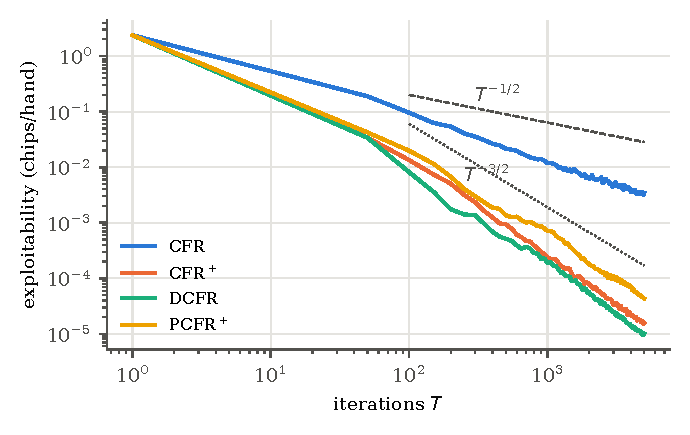
\includegraphics[width=\linewidth]{conv_leduc_iters.pdf}
\column{0.4\textwidth}
The curves show the exploitability of the average strategy for our implementation.

\medskip
After 5{,}000 iterations and \LeducDCFRfiveTime\ seconds DCFR reaches $\LeducDCFRfive$. After 50{,}000 iterations and
\LeducCFRplusLongTime\ seconds CFR$^+$ reaches $\LeducCFRplusLong$ and DCFR $\LeducDCFRLong$.

\medskip
Each extra digit costs about ten times more iterations.
\end{columns}
\note{Exploitability is in chips per hand, and the antes in Leduc are 1 chip.}
\end{frame}

\begin{frame}{Backup: a small river, and every linear solve of one exact solve}
\begin{columns}[c]
\column{0.5\textwidth}
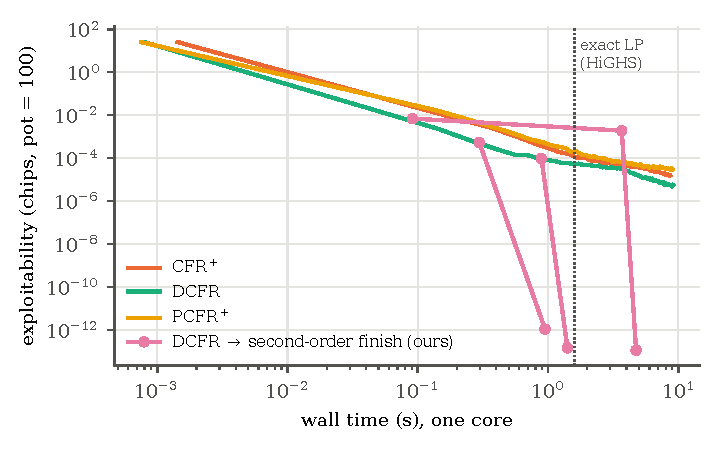
\includegraphics[width=\linewidth]{hybrid_small.pdf}
\column{0.48\textwidth}
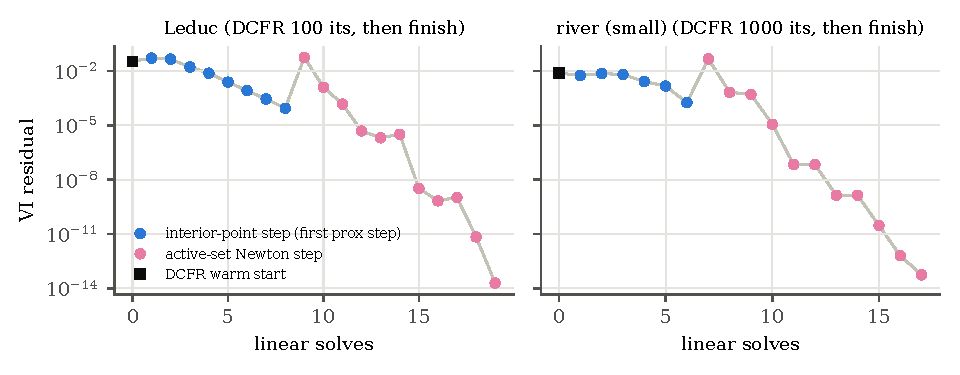
\includegraphics[width=\linewidth]{newton_inner.pdf}
\end{columns}
\medskip
\small On the left is a river with 147 against 139 hands. Our method reaches $\SuppSmallExpl$ chips in \SuppSmallTime\ seconds, DCFR is at
$\SmallDCFRExpl$ after \SmallDCFRTime\ seconds, and the LP takes 1.6 seconds. On the right is the residual after every linear solve. The blue
points are interior-point iterations and the pink points are Newton steps.
\note{The crossover lands on the exact solution of the first regularised
subproblem, whose residual is $\rho\|z^1-z^0\|$, hence the jump. After that each proximal step is solved exactly in one to three steps.}
\end{frame}

\begin{frame}{Backup: the rate of the proximal point method, and why flat equilibria hurt}
The proximal step is the resolvent of a maximal monotone operator $T$, so the iterates move monotonically towards the solution set $Z$.

\medskip
If $T^{-1}$ is upper Lipschitz at $0$ with modulus $a$, which holds for polyhedral problems, then
\[ \operatorname{dist}(z^{k+1}, Z) \ \le\ \frac{a\rho}{\sqrt{1 + a^2\rho^2}}\ \operatorname{dist}(z^k, Z). \]
The modulus $a$ measures how far a point with a small residual can be from $Z$. It is large when the equilibrium set is flat,
that is, when many hands have actions that barely matter.

\medskip
A fast outer loop needs $\rho$ much smaller than $1/a$. But $\|(M+\rho I)^{-1}\|\approx 1/\rho$ then makes the active set of each
subproblem fragile. On Leduc we observe a factor of about $10^{-3}$ for each step at $\rho=10^{-5}$. On the full river of the demonstration no
value of $\rho$ gave both, and the restriction to the support removes the flat directions instead.
\note{Backup for questions about the outer loop. Rockafellar 1976, Luque 1984, Robinson 1981.}
\end{frame}

\end{document}
"
%  This is the simplified deck that goes with the live demonstration (../app). The longer version is talk-detailed.tex.
%  Every number marked "we computed" comes from ../solver (see numbers.tex, generated by gen_numbers.py)
% =====================================================================================
\providecommand\notesmode{0}
\ifnum\notesmode=1 \PassOptionsToClass{handout}{beamer}\fi
\documentclass[10pt,aspectratio=169]{beamer}
\usetheme[progressbar=frametitle,numbering=fraction,block=fill]{metropolis}
\ifnum\notesmode=1
  \setbeameroption{show only notes}
\fi
\usepackage[T1]{fontenc}
\usepackage{lmodern}
\usepackage{amsmath,amssymb,mathtools}
\usepackage{booktabs}
\usepackage{xcolor}
\usepackage{tikz}
\usetikzlibrary{arrows.meta,positioning,calc,shapes.geometric,fit,backgrounds,decorations.pathreplacing}
\usepackage{graphicx}
\usepackage{fancyvrb}
\graphicspath{{../figs/}}
\newcommand{\LeducDCFRfive}{1.0\times 10^{-5}}
\newcommand{\LeducDCFRfiveTime}{14}
\newcommand{\LeducCFRplusLong}{9.2\times 10^{-7}}
\newcommand{\LeducCFRplusLongTime}{130}
\newcommand{\LeducDCFRLong}{1.6\times 10^{-6}}
\newcommand{\LeducHybWarm}{100}
\newcommand{\LeducHybTime}{0.33}
\newcommand{\LeducHybExpl}{5.5\times 10^{-14}}
\newcommand{\LeducHybOuter}{4}
\newcommand{\LeducHybNewton}{19}
\newcommand{\SmallDCFRTime}{9}
\newcommand{\SmallDCFRIters}{30{,}000}
\newcommand{\SmallDCFRExpl}{5.4\times 10^{-6}}
\newcommand{\SmallHybTime}{1.9}
\newcommand{\SmallHybExpl}{3.9\times 10^{-14}}
\newcommand{\SmallHybNewton}{17}
\newcommand{\SmallHybOuter}{6}
\newcommand{\MedDCFRTime}{16}
\newcommand{\MedDCFRExpl}{1.3\times 10^{-4}}
\newcommand{\MedDCFRIters}{5{,}000}
\newcommand{\MedHybTime}{528}
\newcommand{\MedHybExpl}{3.2\times 10^{-5}}
\newcommand{\MedHybOuter}{3}
\newcommand{\MedDCFRLongExpl}{1.8\times 10^{-6}}
\newcommand{\MedDCFRLongTime}{282}
\newcommand{\MedDCFRLongTwoExpl}{3.6\times 10^{-7}}
\newcommand{\MedDCFRLongTwoTime}{520}
\newcommand{\MedDCFRLongTwoIters}{190{,}000}
\newcommand{\MedCFRpLongExpl}{3.8\times 10^{-6}}
\newcommand{\LeducSolves}{19}
\newcommand{\LeducIPM}{8}
\newcommand{\LeducFinishTime}{0.04}
\newcommand{\LeducWarmTime}{0.29}
\newcommand{\SmallSolves}{17}
\newcommand{\SmallIPM}{6}
\newcommand{\SmallFinishTime}{1.58}
\newcommand{\SmallWarmTime}{0.30}
\newcommand{\LeducPure}{49}
\newcommand{\LeducSupport}{59}
\newcommand{\LeducN}{964}
\newcommand{\SmallPure}{71}
\newcommand{\SmallSupport}{52}
\newcommand{\SmallN}{2{,}864}
\newcommand{\SuppLeducTime}{0.30}
\newcommand{\SuppLeducExpl}{6.8\times 10^{-14}}
\newcommand{\SuppLeducRounds}{2}
\newcommand{\SuppLeducWarm}{100}
\newcommand{\SuppLeducSolves}{26}
\newcommand{\SuppSmallTime}{0.95}
\newcommand{\SuppSmallExpl}{1.1\times 10^{-12}}
\newcommand{\SuppSmallRounds}{1}
\newcommand{\SuppSmallWarm}{1{,}000}
\newcommand{\SuppSmallSolves}{16}
\newcommand{\SuppMedTime}{131}
\newcommand{\SuppMedExpl}{2.8\times 10^{-12}}
\newcommand{\SuppMedRounds}{3}
\newcommand{\SuppMedWarm}{3{,}000}
\newcommand{\SuppMedSolves}{163}
\newcommand{\SuppMedFrac}{34}
\newcommand{\SuppMedAdded}{16}
\newcommand{\MedDCFRAtSuppTime}{3.9\times 10^{-6}}
\newcommand{\MedDCFRAtSuppIters}{47{,}490}
\newcommand{\SuppMedOneKTime}{152}
\newcommand{\SuppMedOneKExpl}{3.8\times 10^{-12}}


% ---------- palette (validated categorical slots + inks) ----------
\definecolor{cblue}{HTML}{2A78D6}
\definecolor{corange}{HTML}{EB6834}
\definecolor{caqua}{HTML}{1BAF7A}
\definecolor{cyellow}{HTML}{EDA100}
\definecolor{cmagenta}{HTML}{E87BA4}
\definecolor{ink}{HTML}{0B0B0B}
\definecolor{ink2}{HTML}{52514E}
\definecolor{paper}{HTML}{FCFCFB}
\definecolor{lightblue}{HTML}{CDE2FB}
\definecolor{lightgray}{HTML}{E4E3DF}
\definecolor{felt}{HTML}{1F6B4A}
\definecolor{suitred}{HTML}{C8102E}
\definecolor{suitblue}{HTML}{1C5CAB}
\definecolor{suitgreen}{HTML}{147A3A}
\setbeamercolor{normal text}{fg=ink,bg=paper}
\setbeamercolor{alerted text}{fg=corange}
\setbeamercolor{progress bar}{fg=cblue,bg=lightgray}
\setbeamercolor{frametitle}{bg=ink,fg=paper}
\setbeamercolor{block title}{bg=lightblue,fg=ink}
\setbeamercolor{block body}{bg=lightblue!35,fg=ink}
\setbeamercolor{example text}{fg=caqua!80!black}
\metroset{titleformat frame=regular}
\setbeamerfont{note page}{size=\scriptsize}

% ---------- notation ----------
\newcommand{\src}[1]{{\par\vfill\hfill\tiny\color{ink2}#1}}
\newcommand{\R}{\mathbb{R}}
\newcommand{\ex}{\operatorname{expl}}
\newcommand{\tagP}{\tikz[baseline=-0.6ex]\node[fill=felt,text=white,rounded corners=1.5pt,inner sep=1.6pt,font=\tiny\bfseries]{POKER};}
\newcommand{\tagM}{\tikz[baseline=-0.6ex]\node[fill=cblue,text=white,rounded corners=1.5pt,inner sep=1.6pt,font=\tiny\bfseries]{MATH};}
\newcommand{\tagO}{\tikz[baseline=-0.6ex]\node[fill=corange,text=white,rounded corners=1.5pt,inner sep=1.6pt,font=\tiny\bfseries]{NEW};}

% ---------- playing cards (four-colour deck) ----------
\colorlet{suit-s}{ink}\colorlet{suit-h}{suitred}\colorlet{suit-d}{suitblue}\colorlet{suit-c}{suitgreen}
\newcommand{\suitsym}[1]{\ensuremath{\csname suit@#1\endcsname}}
\makeatletter
\def\suit@s{\spadesuit}\def\suit@h{\heartsuit}\def\suit@d{\diamondsuit}\def\suit@c{\clubsuit}
\makeatother
\newcommand{\pcard}[3][1]{% [scale]{rank}{suit}
  \tikz[baseline=-0.7ex]{\node[draw=ink2,fill=white,rounded corners=2.5pt,minimum width=#1*0.62cm,
  minimum height=#1*0.86cm,inner sep=0pt,text=suit-#3,font=\bfseries\sffamily]
  {\shortstack{#2\\[-1pt]\suitsym{#3}}};}}
\newcommand{\cardback}{\tikz[baseline=-0.7ex]{\node[draw=white,fill=suitred!80!black,rounded corners=2pt,
  minimum width=0.42cm,minimum height=0.6cm,inner sep=0pt]{};}}

\title{Solving Poker}
\subtitle{The numerical analysis behind poker solvers\\ --- and a second-order finish for them}
\author{Numerical Analysis Research Club}
\date{}

\begin{document}

% =====================================================================================
\begin{frame}
  \titlepage
\note{
\textbf{Timing plan for 60 minutes.} Opening and rules 5 $\cdot$ Games, equilibria and the linear program 9 $\cdot$
Regret minimisation and CFR 9 $\cdot$ Live demonstration 12 $\cdot$ The new method 13 $\cdot$ Results, limits and wrap-up 8.
That leaves about four minutes for questions during the talk.\\[4pt]
If running late, shorten the demonstration to its five minute version (see \texttt{app/DEMO\_NOTES.md}) and give the slide
``Making it robust and fast'' one sentence.\\[4pt]
Opening line: ``Ten years ago the best poker players in the world lost to programs whose core is a few lines of
arithmetic repeated a few billion times. This talk is about that arithmetic, read as numerical analysis, and about
what a numerical analyst can add to it.''\\[4pt]
The slides alternate between \textsc{poker} (green tag) and \textsc{math} (blue tag). The orange tag \textsc{new} marks
our own contribution. Every number that we computed comes from the Python solver in the repository. The more detailed
version of this deck, with all citations and extra slides, is \texttt{talk-detailed.pdf}.
}
\end{frame}

% =====================================================================================
\begin{frame}{\tagP\ Ten years of superhuman poker}
\begin{columns}[T]
\column{0.58\textwidth}
In 2015 a program called Cepheus essentially solved two-player limit hold'em.

\medskip
In 2017 two programs, DeepStack and Libratus, beat professional players at the no-limit game, which is far larger.
In 2019 Pluribus did the same at a table of six.

\medskip
Today every serious player studies with a \alert{solver}. You describe one situation, and the program computes how
to play every possible hand in it.

\medskip
All of these programs share one simple iteration. This talk explains it and then tries to improve on it.
\column{0.4\textwidth}
\centering
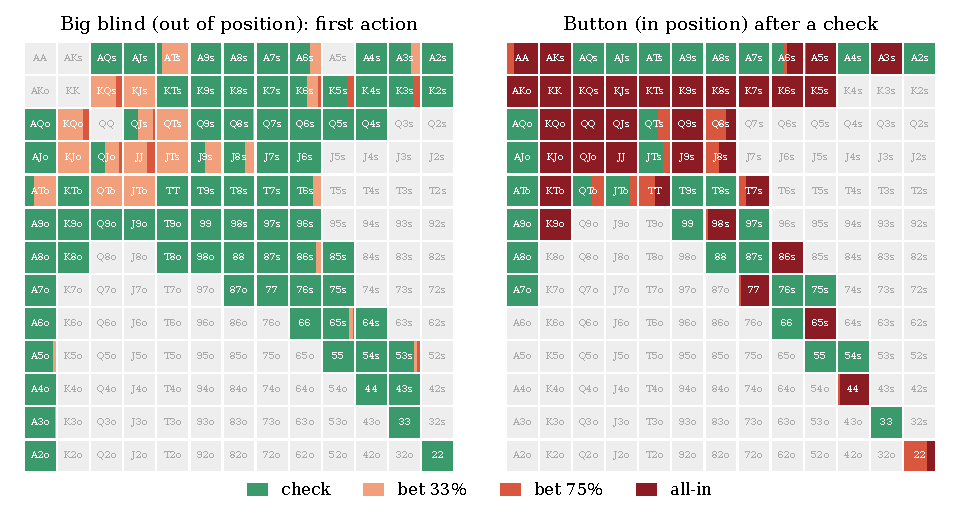
\includegraphics[height=0.6\textheight,trim=0 22 245 0,clip]{grid_root.pdf}\\[-2pt]
{\scriptsize\color{ink2} A solver's answer, computed by our own code. Each square is a starting hand and the colours are actions.}
\end{columns}
\note{
The common core of all these programs is an iterative method, counterfactual regret minimisation, applied to a very large
saddle-point problem. Libratus and DeepStack add abstraction (shrinking the game) and subgame solving
(solving again the part of the game you are actually in), but the inner loop is still a method of the CFR family.\\[3pt]
Commercial solvers such as PioSolver, GTO+ and GTO Wizard are what human players use. You give the board, the
two ranges and the allowed bet sizes, and the program computes an equilibrium of that subgame. The picture on the right is
exactly such an output, produced by our solver for the river situation that we use for the whole talk.\\[3pt]
References if asked: Bowling et al., Science 2015. Morav\v{c}\'ik et al., Science 2017. Brown and Sandholm, Science 2018 and 2019.
}
\end{frame}

% =====================================================================================
\begin{frame}{The plan: poker $\leftrightarrow$ math}
\centering
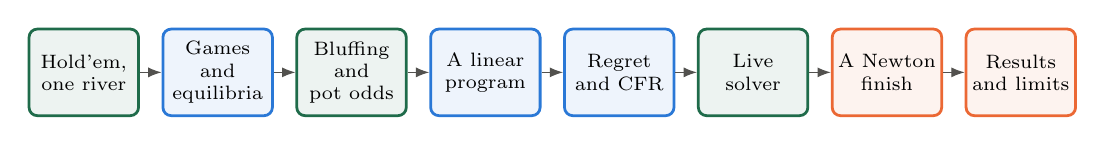
\begin{tikzpicture}[x=1cm,y=1cm,every node/.style={font=\scriptsize}]
  \foreach \i/\t/\c in {0/{Hold'em,\\ one river}/felt, 1/{Games and\\ equilibria}/cblue, 2/{Bluffing and\\ pot odds}/felt,
                       3/{A linear\\ program}/cblue, 4/{Regret\\ and CFR}/cblue, 5/{Live\\ solver}/felt,
                       6/{A Newton\\ finish}/corange, 7/{Results\\ and limits}/corange}{
    \node[draw=\c,line width=1pt,rounded corners=3pt,text width=1.25cm,minimum height=1.1cm,align=center,
          inner sep=2pt,fill=\c!8] (n\i) at (1.7*\i,0) {\t};
  }
  \foreach \i [evaluate=\i as \j using int(\i+1)] in {0,...,6} { \draw[-{Latex},ink2] (n\i) -- (n\j); }
\end{tikzpicture}

\vspace{1.4em}
\raggedright
The equilibrium of a poker game is the solution of a very large and very structured saddle-point problem.
Solvers attack it with a first-order method whose steps are cheap and whose last digits are slow.

\medskip
In the middle of the talk we solve a real hand live in the browser and look at the answer together.

\medskip
Our own contribution comes last. We treat the end of the solve as a nonsmooth equation and finish it with a Newton
method, which reaches machine precision where the first-order method would need millions of iterations.
\note{
Say what the audience will get. First, enough poker to read the output of a solver. Second, the mathematics of why CFR converges
and why it is fast in practice. Third, a live demonstration in which they can ask for any change to the hand. Fourth, a new method
from the numerical optimisation toolbox, with honest results: where it wins by orders of magnitude, and where it does not yet.
}
\end{frame}

% =====================================================================================
\begin{frame}{\tagP\ Texas hold'em in one slide}
\begin{columns}[T]
\column{0.5\textwidth}
Each of the two players is dealt two private cards. Five public cards, the \emph{board}, are then revealed in three
stages called the flop, the turn and the river.

\medskip
There is a round of betting before the flop and after each stage. A player may check, bet, call, raise or fold, and in the
no-limit game a bet can be any size up to the player's stack.

\medskip
If nobody folds, the best five-card hand made from the seven available cards wins the pot.
\column{0.48\textwidth}
\centering
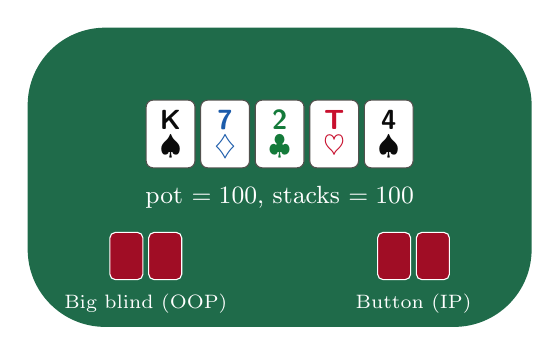
\begin{tikzpicture}
  \fill[felt,rounded corners=28pt] (-3.2,-1.9) rectangle (3.2,1.9);
  \node at (0,0.55) {\pcard{K}{s}\,\pcard{7}{d}\,\pcard{2}{c}\,\pcard{T}{h}\,\pcard{4}{s}};
  \node[text=white,font=\small] at (0,-0.25) {pot $= 100$, stacks $= 100$};
  \node at (-1.7,-1.0) {\cardback\,\cardback};
  \node at (1.7,-1.0) {\cardback\,\cardback};
  \node[text=white,font=\scriptsize] at (-1.7,-1.6) {Big blind (OOP)};
  \node[text=white,font=\scriptsize] at (1.7,-1.6) {Button (IP)};
\end{tikzpicture}\\[4pt]
{\small Our running example is the \alert{river}, the last round of betting.\\
The big blind acts first, which is called being out of position.}
\end{columns}
\note{
Keep this light, since most of the audience has played or watched poker. The key structural fact is that the board is
public and the two hole cards are private. A strategy must therefore be a function of
the public history and your own cards. You do not know the opponent's cards, only a probability distribution over them,
which poker players call a \textbf{range}.\\[3pt]
The river situation is fixed for the whole talk: board K$\spadesuit$ 7$\diamondsuit$ 2$\clubsuit$ T$\heartsuit$ 4$\spadesuit$, pot 100, both players
have 100 behind. The big blind may check or bet 33\% or 75\% of the pot or go all-in. Facing a bet you may fold, call or go all-in.
The live demonstration uses exactly this table.
}
\end{frame}

% =====================================================================================
\begin{frame}{\tagP\ Ranges: what a solver takes as input}
\begin{columns}[T]
\column{0.6\textwidth}
\centering
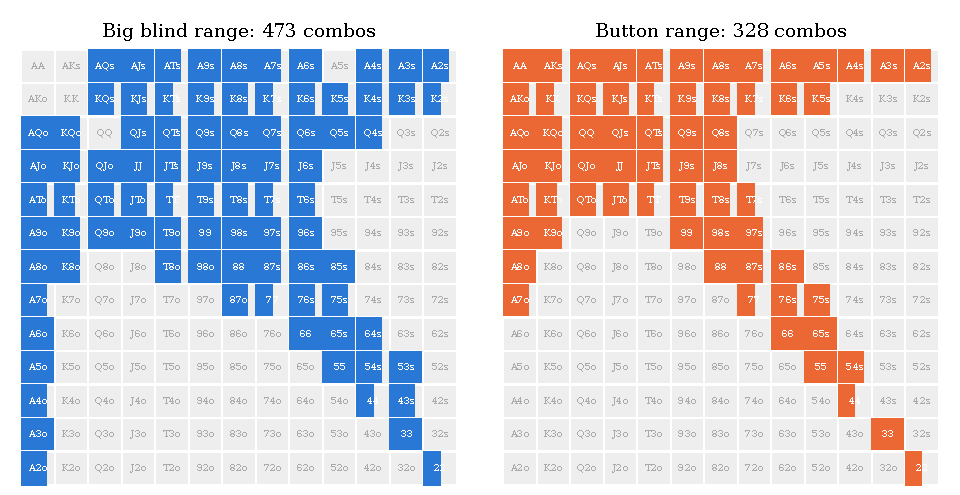
\includegraphics[width=\linewidth]{ranges.pdf}
\column{0.38\textwidth}
A \textbf{range} is a probability vector over the two-card hands a player can hold. There are 1326 such hands, and 1081
once the five board cards are known.

\medskip
In our example the big blind called a raise before the flop and the button made that raise, so the two ranges are
different.

\medskip
The solver returns, for every point of the betting and for every hand, a probability for each action.
\end{columns}
\note{
The 13 by 13 grid is the standard poker picture. Pairs are on the diagonal, suited hands above it and offsuit hands below it.
Each cell is a class of hands, for example AKs stands for 4 combinations. Mathematically the input is two nonnegative vectors
$r_1\in\R^{n_1}$ and $r_2\in\R^{n_2}$. Two hands that share a card cannot both be dealt, which is called card removal, and it is a 0/1
compatibility matrix $C$ between the ranges. Both will appear in the formulas later.\\[3pt]
The width of each bar shows how many combinations are still possible given the board. The king of spades is on the board, so there
are fewer hands with a king.
}
\end{frame}

% =====================================================================================
\begin{frame}{\tagM\ Two-player zero-sum games and Nash equilibrium}
Each player chooses a strategy from a compact convex set, $x\in X$ and $y\in Y$, and the first player receives the
bilinear payoff $x^\top A y$ from the second.
\begin{block}{Minimax theorem (von Neumann 1928)}
\[ \max_{x\in X}\min_{y\in Y} x^\top A y \;=\; \min_{y\in Y}\max_{x\in X} x^\top A y \;=:\; v^\ast . \]
\end{block}
A pair $(x^\ast,y^\ast)$ that attains both sides is a \textbf{Nash equilibrium}, and $v^\ast$ is the value of the game.
Playing $x^\ast$ guarantees at least $v^\ast$ against any opponent, which is what poker players mean by an unexploitable strategy.
\begin{block}{The error that every solver reports is the exploitability}
\[\ex(x,y) \;=\; \tfrac12\Big(\max_{x'} x'^\top A y \;-\; \min_{y'} x^\top A y'\Big)\;\ge 0 ,
  \qquad\text{with equality exactly at an equilibrium.}\]
\end{block}
\note{
For an applied mathematics audience this is a convex-concave saddle-point problem with a bilinear coupling, and the exploitability
is the primal-dual gap. Everything later is a method for driving this gap to zero. Its unit is chips per hand.\\[3pt]
Practical solvers stop at an exploitability of a fraction of a percent of the pot. We will push to $10^{-13}$.
Our numbers are in chips with a pot of 100, so $10^{-2}$ chips is $10^{-4}$ of the pot.
}
\end{frame}

% =====================================================================================
\begin{frame}{\tagP\ Why equilibria mix: bluffing and pot odds}
\begin{columns}[T]
\column{0.56\textwidth}
Take a toy river with a pot of 1. The bettor holds either the best hand or nothing and bets $s$. The caller holds a
medium hand that only beats a bluff.

\medskip
The caller is indifferent between calling and folding when bluffs are a fraction $\beta = \dfrac{s}{1+2s}$ of the bets.

\medskip
The bettor's bluffs are indifferent when the caller continues with probability $\dfrac{1}{1+s}$. Poker players call
this the \emph{minimum defence frequency}.

\medskip
Any pure strategy can be exploited here. The equilibrium randomises, and it does so exactly where the opponent
is made indifferent.
\column{0.4\textwidth}
\centering
\begin{tabular}{ccc}
\toprule
bet $s$ & bluffs $\beta$ & defend \\ \midrule
$1/3$ & 20\% & 75\% \\
$3/4$ & 30\% & 57\% \\
$1$ & 33\% & 50\% \\
$2$ & 40\% & 33\% \\ \bottomrule
\end{tabular}\\[10pt]
{\small We will check the last column against the live solver.}
\end{columns}
\note{
Derivation, to say and not to write. For the caller, calling wins $1+s$ against a bluff and loses $s$ against a value bet.
The caller is indifferent when $\beta(1+s) = (1-\beta)s$, which gives $\beta = s/(1+2s)$. For the bettor with nothing, betting wins the pot $1$
when the caller folds and loses $s$ when called, and checking wins nothing. The bettor is indifferent when $(1-c)\cdot 1 = c\, s$, which gives $c = 1/(1+s)$.\\[3pt]
The mathematical point: at an equilibrium every action played with positive probability is a best response. This is
complementary slackness in the linear program that we are about to write down. Mixing happens exactly where reduced costs vanish.
}
\end{frame}

% =====================================================================================
\begin{frame}{\tagM\ Games on trees with hidden information}
\begin{columns}[T]
\column{0.52\textwidth}
Poker is a game tree. Chance deals the cards, the players act in turn, and the leaves carry the payoffs.

\medskip
A player cannot see the opponent's cards, so several nodes look the same to that player. Such a group of
nodes is an \textbf{information set}, and a strategy assigns a probability distribution over actions to each one.

\medskip
{\footnotesize
\begin{tabular}{lr}
\toprule
game & information sets \\ \midrule
Kuhn poker & 12 \\
Leduc hold'em & 288 \\
Limit hold'em & $3.2\times10^{14}$ \\
No-limit hold'em & about $10^{161}$ \\ \bottomrule
\end{tabular}}
\column{0.46\textwidth}
\centering
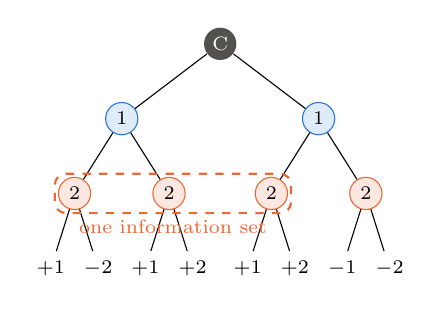
\begin{tikzpicture}[level distance=0.95cm,
   level 1/.style={sibling distance=2.5cm},level 2/.style={sibling distance=1.2cm},level 3/.style={sibling distance=0.6cm},
   every node/.style={font=\scriptsize}]
  \node[circle,fill=ink2,text=white,inner sep=1.5pt] {C}
    child { node[circle,draw=cblue,fill=cblue!15,inner sep=2pt] (a) {1}
       child { node[circle,draw=corange,fill=corange!15,inner sep=2pt] (b1) {2} child{node{$+1$}} child{node{$-2$}} }
       child { node[circle,draw=corange,fill=corange!15,inner sep=2pt] (b2) {2} child{node{$+1$}} child{node{$+2$}} } }
    child { node[circle,draw=cblue,fill=cblue!15,inner sep=2pt] (c) {1}
       child { node[circle,draw=corange,fill=corange!15,inner sep=2pt] (d1) {2} child{node{$+1$}} child{node{$+2$}} }
       child { node[circle,draw=corange,fill=corange!15,inner sep=2pt] (d2) {2} child{node{$-1$}} child{node{$-2$}} } };
  \draw[corange,dashed,thick,rounded corners] ($(b1)+(-0.25,0.25)$) -- ($(d1)+(0.25,0.25)$) -- ($(d1)+(0.25,-0.25)$) -- ($(b1)+(-0.25,-0.25)$) -- cycle;
  \node[corange,font=\scriptsize] at ($(b1)!0.5!(d1)+(0,-0.42)$) {one information set};
\end{tikzpicture}\\[2pt]
{\scriptsize Player 2 sees the action of player 1 but not the deal.}
\end{columns}
\note{
Leduc hold'em is the standard research benchmark. It has a deck of six cards, one private
card each, one public card, and two betting rounds. It has 288 information sets and we use it as our small test problem.\\[3pt]
The size column is the reason the subject exists. Nobody can write down no-limit hold'em. Real systems solve an abstraction
in which similar hands and bet sizes are merged, and then solve subgames like our river again during play.\\[3pt]
We assume perfect recall: a player never forgets what he knew or did. Sizes are from Bowling et al.\ 2015 and Johanson 2013.
Kuhn and Leduc were counted by our code.
}
\end{frame}

% =====================================================================================
\begin{frame}{\tagM\ The sequence form: equilibrium is a linear program}
Give player 1 one variable $x_\sigma$ for each \emph{sequence} $\sigma$ of her own
actions, equal to the product of her probabilities along it. These variables satisfy linear flow constraints
$Ex = e$, $x\ge 0$, and the expected payoff is bilinear in them, $u(x,y) = x^\top A y$.
\begin{block}{Theorem (Koller, Megiddo and von Stengel 1996)}
An equilibrium strategy of player 1 solves
\[\max_{x,\,q}\ f^\top q\quad \text{subject to}\quad A^\top x - F^\top q \ge 0,\quad Ex = e,\quad x\ge 0 ,\]
a linear program whose size is \emph{linear} in the size of the game tree.
\end{block}
So why not call an LP solver? On our river $A$ has 2.9 million nonzeros, because every leaf couples every hand of one
player to every hand of the other, and a good LP code did not finish in 25 minutes. The iteration we describe next
reaches $\MedDCFRExpl$ chips in \MedDCFRTime\ seconds.
\note{
This is the key modelling step. Mixed strategies over the pure strategies of the normal form would have exponentially many
variables. Realisation plans have one variable per sequence, and perfect recall makes the payoff bilinear in them.\\[3pt]
$E$ and $F$ are very sparse, with one row per information set and entries $\pm1$, and they encode flow conservation on a tree.
$A$ is where the poker lives. The program has 17{,}626 unknowns on our river. Say that the dual variables $q$ are the values of the opponent's information sets, and remember them: they are values of information sets, the same quantities
that CFR computes in every iteration. This is how we will warm-start the duals later.\\[3pt]
The LP run used HiGHS through SciPy with default settings on one core and we stopped it after 25 minutes. On the smaller test
problems the LP is perfectly fine: 0.04 s on Leduc and 1.6 s on a small river. The DCFR figure is for \MedDCFRIters\ iterations.
}
\end{frame}

% =====================================================================================
\begin{frame}{\tagM\ Regret matching}
\begin{columns}[T]
\column{0.62\textwidth}
We face the same decision many times. The \emph{regret} $R_T(a)$ of an action is how much better it would have done
than what we played. Regret matching plays each action in proportion to its positive regret.
{\small\[ R_T(a) = \sum_{t=1}^T \big(u_t(a) - u_t(\sigma_t)\big),\quad
   \sigma_{T+1}(a) = \frac{[R_T(a)]^+}{\sum_b [R_T(b)]^+}. \]}
\begin{block}{Theorem (Hart and Mas-Colell 2000)}
The regrets grow only like $\sqrt{T}$: $\ \max_a R_T(a) \le \Delta\sqrt{|A|\,T}$.
\end{block}
When both players of a zero-sum game do this, their \emph{average} strategies converge to an equilibrium.
\column{0.36\textwidth}
\centering
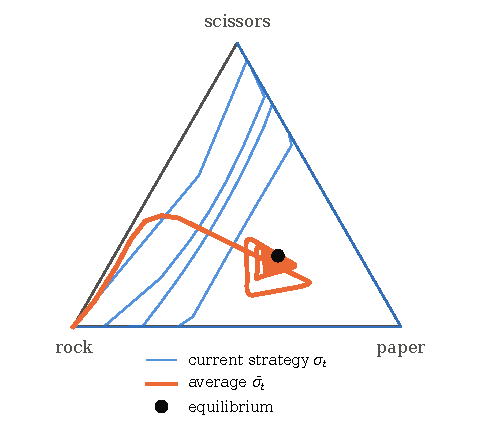
\includegraphics[width=\linewidth]{rm_rps.pdf}\\
{\scriptsize Our computation on a weighted rock-paper-scissors game. The current strategy cycles and the average converges.}
\end{columns}
\note{
Idea of the proof. The regret vector satisfies $\|[R_{T}]^+\|^2 \le \|[R_{T-1}]^+\|^2 + \Delta^2|A|$ because the
cross term $\langle [R_{T-1}]^+, r_T\rangle$ vanishes by the choice of $\sigma_T$: the instantaneous regret is orthogonal to the
current positive regrets. Sum and take square roots. This is Blackwell approachability, and $\Delta$ is the range of the payoffs.\\[3pt]
The folk theorem: if both players have average regret at most $\varepsilon$ then the average strategies are a $2\varepsilon$-equilibrium,
because $\max_{x'} x'^\top A \bar y - \min_{y'} \bar x^\top A y' \le 2\varepsilon$.\\[3pt]
In the figure the limit is $(\frac14,\frac12,\frac14)$.
}
\end{frame}

% =====================================================================================
\begin{frame}{\tagM\ Counterfactual regret minimisation (CFR)}
CFR runs regret matching separately at every information set $I$. The payoff it feeds to each one is the
\textbf{counterfactual value} of an action, which is the expected payoff weighted by the probability that the opponent and
chance lead to $I$, as if the player herself had tried to get there.
\[ v_i(\sigma, I, a) = \sum_{h\in I}\ \pi_{-i}^{\sigma}(h)\sum_{z \sqsupset ha} \pi^{\sigma}(ha\to z)\, u_i(z) \]
\begin{block}{Theorem (Zinkevich, Johanson, Bowling and Piccione 2007)}
The regret of the whole strategy is at most the sum of the local regrets. Therefore the average strategies satisfy
\[ \ex(\bar x_T,\bar y_T) \ \le\ \frac{\Delta\,|\mathcal I|\sqrt{|A|}}{\sqrt T}. \]
\end{block}
One iteration is one pass over the tree, with reach probabilities computed on the way down and values on the way up.
The matrix $A$ is never formed.
\note{
The decomposition is the whole trick. A global regret over an exponentially large strategy space is bounded by a sum of small
local regrets, and each of them is minimised by plain regret matching. This is why CFR scales: the cost of an iteration is linear in the tree
and so is the storage, two numbers for each information set and action.\\[3pt]
In the language of linear algebra, one CFR iteration computes $Ay$ and $A^\top x$ for the current realisation plans by walking the tree.
These are the same two products that any first-order saddle-point method needs.
}
\end{frame}

% =====================================================================================
\begin{frame}{\tagP\tagM\ CFR for poker: one pass for all hands}
In poker the betting is public and only the cards are hidden. At each point of the betting we store
\emph{vectors} indexed by hands, such as the reach probabilities $\pi_1$ and $\pi_2$.
At a leaf the values of all hands come from one matrix-vector product.
\[ v_1 = \text{amount}\cdot B\,\pi_2,\qquad
   B_{ij} = \underbrace{C_{ij}}_{\text{no shared card}}\cdot\begin{cases} 1 & \text{after a fold}\\ \operatorname{sign}(s_i - s_j) & \text{at a showdown}\end{cases} \]
Here $s_i$ is the strength of hand $i$. The matrix $B$ is dense but very structured. Once the hands are sorted by
strength, the sign matrix is all ones below the diagonal and all minus ones above it, and $C$ is the all-ones matrix
minus a sparse correction for hands that share a card.

\medskip
As a result $B\pi$ costs one sort and a running sum, which is $O(n\log n)$ operations and not $n^2$.
\note{
This is the bridge between the tree picture and the implementation. The information sets at a public node are indexed by the
private hand of the player to act, so all information sets at this node form a vector and every CFR operation becomes a vector operation.\\[3pt]
This is also the poker-specific numerical linear algebra. Each terminal block is low rank plus sparse. The fold block is
rank one minus a sparse correction. The showdown block, after sorting, is a sign matrix, which is semiseparable (think of the inverse of
a bidiagonal matrix), times the compatibility mask. The trick is due to Johanson et al.\ 2011.\\[3pt]
The public tree itself is drawn live in the demonstration, so it is not on a slide any more. It has 12 decision points and 21 leaves, and one iteration takes about a millisecond in the browser. Keep in mind that this structure is what a
scalable Newton method would have to exploit, which comes back at the end of the talk.
}
\end{frame}

% =====================================================================================
\begin{frame}{\tagM\ Four variants of one loop}
Modern solvers change how CFR weights the old regrets and how it averages the strategies.

\smallskip
\renewcommand{\arraystretch}{1.15}\small
\begin{tabular}{p{1.5cm}p{6.4cm}p{5.0cm}}
\toprule
method & what changes & a numerical analyst would say \\ \midrule
CFR$^+$ & Negative regrets are reset to zero and later strategies get more weight in the average. & projection onto the nonnegative orthant \\
DCFR & Old regrets and old strategies are multiplied by factors below one. & forgetting factors that damp the transient \\
PCFR$^+$ & The strategy is computed from the regrets plus a prediction of the next regret. & optimism, as in the extragradient method \\ \bottomrule
\end{tabular}

\smallskip
\normalsize The proven rate is still $T^{-1/2}$ for all four. In practice the modern variants are much faster, and we will
now race them against each other on a real hand.
\note{
CFR$^+$ (Tammelin 2014) is what solved limit hold'em. DCFR (Brown and Sandholm 2019) with parameters $(1.5, 0, 2)$ is the default in many solvers:
positive regrets are multiplied by $t^{1.5}/(t^{1.5}+1)$, negative ones by $1/2$, and the average by $(t/(t+1))^2$.
PCFR$^+$ (Farina, Kroer and Sandholm 2021) uses the last instantaneous regret as its prediction and connects regret matching to optimistic mirror descent.\\[3pt]
All four also update the two players in turn, so that the second player already sees the new strategy of the first, which is Gauss-Seidel in place of Jacobi.\\[3pt]
The observed rates are between $T^{-1}$ and $T^{-3/2}$ for the averages, while the last iterate oscillates. Explaining this gap to the
theory is an open question. The rates are still sublinear, and that is the gap our method addresses.
}
\end{frame}

% =====================================================================================
\begin{frame}{\tagP\tagM\ Live demonstration: the river solver table}
\begin{columns}[c]
\column{0.55\textwidth}
\centering
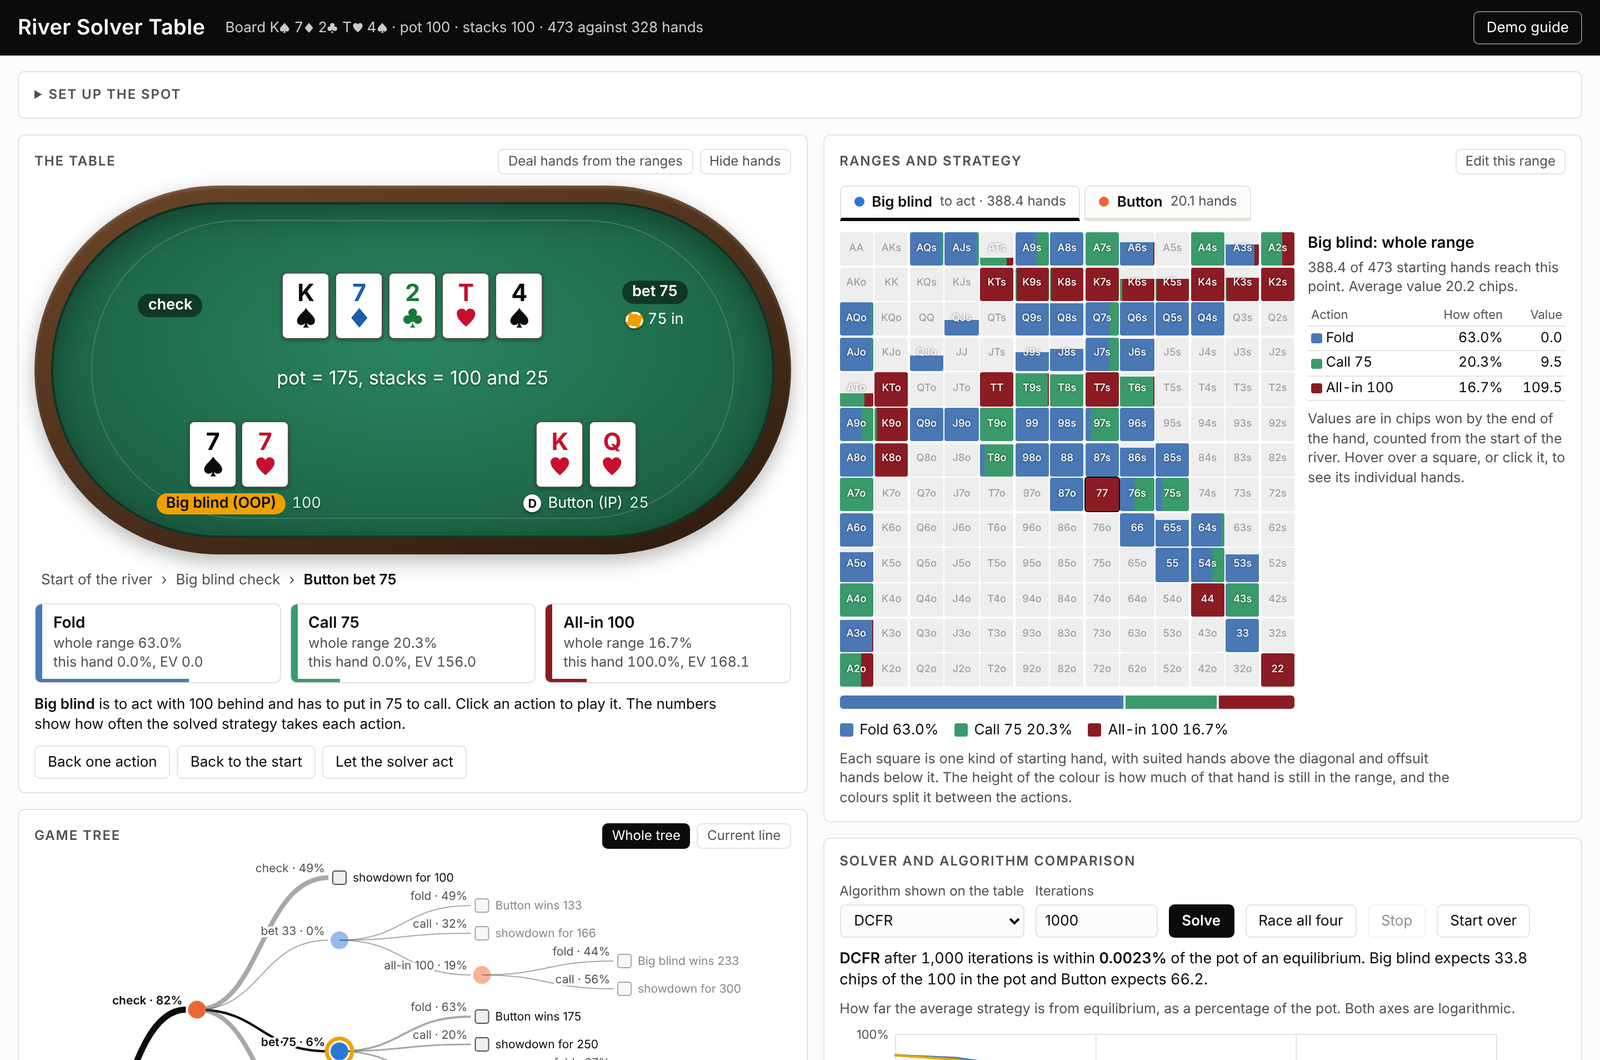
\includegraphics[width=\linewidth]{app_slide.png}
\column{0.43\textwidth}
The page \texttt{app/poker-solver.html} solves our river in the browser. It will answer five questions.
\begin{enumerate}\small\setlength\itemsep{2pt}
\item Which of the four algorithms wins a race?
\item What does the big blind do with each of its 473 hands?
\item How do the ranges and the tree change as the hand is played?
\item Does a hand that mixes get the same value from both actions?
\item Does the solver agree with the pot odds formula?
\end{enumerate}
After that the board, the ranges and the bet sizes are yours to change.
\end{columns}
\note{
Switch to the browser now. The full script with what to click and what to say is in \texttt{app/DEMO\_NOTES.md} (also as a PDF),
and the same steps are in the Demo guide inside the page. Budget twelve minutes.\\[3pt]
Short version of the script. (1) Load the page, which solves the spot with DCFR in two seconds. Point at the table, the grid, the tree and the chart.
(2) Press Race all four. After 1000 iterations CFR is at about 0.11\% of the pot, PCFR$^+$ at 0.009\%, CFR$^+$ at 0.007\% and DCFR at 0.002\%.
(3) Read the big blind's grid: check 82\%, bet a third of the pot 16\%, bet three quarters 2\%. Value bets and bluffs.
(4) Give the big blind three sevens: it checks every time, and after the button bets 75 it raises all-in every time.
(5) After check and bet 75, select ace-nine offsuit: it folds 63\% and calls 37\%, and both actions are worth 0.0 chips.
(6) After the big blind bets 33, the button folds 26\%, and the formula says at most 25\%. After a check and an all-in the big blind folds 68\%, far more than the formula's 50\%.
(7) Change the river card to the nine of hearts and solve again. Then take requests from the audience.\\[3pt]
If the browser fails, the static grids are in \texttt{talk-detailed.pdf}, slides 18 and 19.
}
\end{frame}

% =====================================================================================
\begin{frame}{\tagP\ What the demonstration showed}
\begin{columns}[T]
\column{0.42\textwidth}
The solution reads like poker. Strong hands bet, a few hands with nothing bluff, and the hands in between check.

\medskip
A hand that mixes two actions gets the same value from both. This is complementary slackness.

\medskip
The button defends within 1.5 points of the pot odds formula. The big blind folds much more than the formula says,
because the button's bluffs would still win some showdowns by checking.
\column{0.57\textwidth}
\centering
{\scriptsize\setlength\tabcolsep{3pt}
\begin{tabular}{@{}llccc@{}}
\toprule
defender & line & $s$ & defends & MDF \\ \midrule
Button & BB checks, BTN bets 75, BB jams & $0.10$ & $64.7\%$ & $90.9\%$ \\
Button & BB bets 33 & $0.33$ & $74.3\%$ & $75.2\%$ \\
Button & BB checks, BTN bets 33, BB jams & $0.40$ & $57.8\%$ & $71.2\%$ \\
Button & BB bets 75 & $0.75$ & $55.8\%$ & $57.1\%$ \\
Button & BB bets 100 & $1.00$ & $49.1\%$ & $50.0\%$ \\
Big blind & BB bets 75, BTN jams & $0.10$ & $63.4\%$ & $90.9\%$ \\
Big blind & BB checks, BTN bets 33 & $0.33$ & $52.2\%$ & $75.2\%$ \\
Big blind & BB bets 33, BTN jams & $0.40$ & $56.3\%$ & $71.2\%$ \\
Big blind & BB checks, BTN bets 75 & $0.75$ & $37.5\%$ & $57.1\%$ \\
Big blind & BB checks, BTN bets 100 & $1.00$ & $32.6\%$ & $50.0\%$ \\
\bottomrule
\end{tabular}
}\\[6pt]
{\scriptsize Exact equilibrium of our river. Here $s$ is the bet as a fraction of the pot, MDF is $1/(1+s)$, and a jam is an all-in bet.}
\end{columns}
\note{
This is a consistency check of the whole pipeline. When the big blind bets, the button defends 74.3\% against 75.2\%, 55.8\% against
57.1\% and 49.1\% against 50.0\%, so the toy formula is almost exact. When the button bets after a check, the big blind folds much
more. We checked that the button's weakest betting hands mix between checking and going all-in, so the indifference that fixes
the defence frequency is ``value of the all-in equals value of checking, which is positive'' and not ``value of the all-in equals zero''.\\[3pt]
The numbers in the table come from the exact equilibrium computed by the method of the next part, so they can differ in the last digit from what the
browser showed after 1000 iterations.
}
\end{frame}

% =====================================================================================
\begin{frame}{\tagM\ Why push the precision further?}
\begin{columns}[T]
\column{0.58\textwidth}
Practical solvers stop at about 0.1\% of the pot, and for a human studying a hand that is plenty.

\medskip
More digits matter when a program stitches many small solves together and their errors add up, when we ask exactly which
hands mix, and when research needs a ground truth with a certificate.

\medskip
For a numerical analyst, CFR is a first-order method on a nonsmooth and degenerate problem. It is
robust and cheap, and its tail is sublinear. The classical cure for a slow tail is a \alert{local method of higher
order}, started from a good point.
\column{0.4\textwidth}
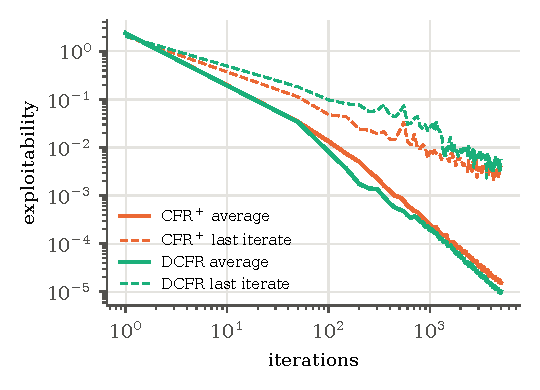
\includegraphics[width=\linewidth]{avg_vs_last.pdf}\\
{\scriptsize Our computation on Leduc. Only the average converges, and each extra digit costs about ten times more iterations.}
\end{columns}
\note{
Make the case without overselling. Precision matters for machines (solving subgames again, evaluation) and for science
(knowing the exact equilibrium, for example the exact bluffing frequencies, or whether a hand mixes at all).\\[3pt]
The analogy for this audience: CFR is like a stationary iterative method. It is fantastic for the first
digits and hopeless for the last ones, and the obvious idea is to switch to a Newton-type method near the solution.\\[3pt]
Numbers for Leduc: CFR$^+$ reaches $\LeducCFRplusLong$ after 50{,}000 iterations and \LeducCFRplusLongTime\ seconds. The curves are on a backup slide.
}
\end{frame}

% =====================================================================================
\begin{frame}{\tagO\ Step 1: write the equilibrium as a variational inequality}
Collect both strategies and both vectors of information-set values in one unknown $z = (x, y, p, q)$. An
equilibrium is a point that satisfies the optimality conditions of both players' linear programs.
\[
\begin{aligned}
 0\le x \ &\perp\ E^\top p - A y \ \ge 0, & Ex &= e,\\
 0\le y \ &\perp\ A^\top x - F^\top q \ \ge 0, & Fy &= f.
\end{aligned}
\]
These conditions have the form $w = Mz + b$ with a matrix that is \textbf{skew-symmetric}.
\[ M = \begin{pmatrix} 0 & -A & E^\top & 0\\ A^\top & 0 & 0 & -F^\top\\ -E & 0 & 0 & 0\\ 0 & F & 0 & 0\end{pmatrix},
   \qquad M + M^\top = 0 . \]
Skew symmetry makes the problem monotone. It also means that the solutions form a polyhedron and
not a single point, so Newton's method cannot be applied directly. CFR gives a starting point for all of $z$ for free.
\note{
This is a mixed linear complementarity problem. The reduced cost $E^\top p - Ay$ of a sequence is its counterfactual
regret scaled by reach, and complementarity says ``play only actions with zero regret''. So CFR and this system talk
about the same quantities: the CFR average strategies are $x$ and $y$, and its best-response values are $p$ and $q$.\\[3pt]
Skewness: the $x$-$y$ block is the zero-sum coupling. The $(x,p)$ and $(y,q)$ blocks are pairs of constraints and multipliers, arranged
with signs so that $M^\top = -M$.\\[3pt]
Non-uniqueness is already visible in Kuhn poker, where the equilibria form a one-parameter family (backup slide).\\[3pt]
If asked what we tried first: Anderson acceleration of the CFR$^+$ map, vector extrapolation of the averages, and Levenberg-Marquardt on the
optimality system. None of them beat DCFR on Leduc. The CFR map is piecewise linear with non-isolated fixed points, and the acceleration theory needs a smooth contraction.
The details are in \texttt{talk-detailed.pdf}.
}
\end{frame}

% =====================================================================================
\begin{frame}{\tagO\ Step 2: the proximal point method makes each problem well posed}
We add a small multiple of the identity. Given $z^k$, the next iterate $z^{k+1}$ solves the same conditions with
\[ w_\rho(z) = (M + \rho I)\,z + b - \rho\, z^{k} . \]
\begin{columns}[T]
\column{0.56\textwidth}
Since $d^\top(M+\rho I)d = \rho\|d\|^2$, the matrix $M+\rho I$ is positive definite and each regularised problem
has exactly one solution.

\medskip
\textbf{Theorem (Rockafellar 1976, Luque 1984).} The iterates converge to a solution of the original problem for every
$\rho>0$. For a polyhedral problem the rate is linear, with a factor that tends to zero with $\rho$.

\medskip
A small $\rho$ gives a fast outer loop and badly conditioned inner problems.
\column{0.41\textwidth}
\begin{block}{Our computation on Leduc with $\rho = 10^{-5}$}
\small The residual after each outer step:\\[2pt]
$3.4\!\times\!10^{-2} \to 4.8\!\times\!10^{-6} \to 3.3\!\times\!10^{-9}$\\ $\to 6.9\!\times\!10^{-12} \to 2.0\!\times\!10^{-14}$\\[3pt]
About three digits for each step.
\end{block}
\end{columns}
\note{
The proximal term fixes the non-uniqueness. Each subproblem has exactly one solution, so Newton's method has a well defined and
nonsingular target. For polyhedral monotone problems the inverse operator is upper Lipschitz (Robinson 1981), which gives linear
convergence of the proximal point method with a factor that tends to zero as $\rho\to0$.\\[3pt]
The trade-off is the whole story of the last part of the talk. A small $\rho$ makes the outer loop fast and the inner problems
nearly as ill posed as the original one, since $\|(M+\rho I)^{-1}\|\le 1/\rho$. There is a backup slide with the rate.
}
\end{frame}

% =====================================================================================
\begin{frame}{\tagO\ Step 3: Newton's method on a piecewise-linear equation}
Each regularised problem can be written as one equation. For every action, either its probability is zero or its
reduced cost is zero, and that is the same as $\min\big(x_i,\ w_\rho(z)_i\big)=0$.

\medskip
A Newton step for this equation guesses which actions are dropped, imposes indifference on all the others, and solves
one linear system. Its matrix has the form $V = D_a + D_b(M+\rho I)$ with nonnegative diagonal matrices $D_a$ and $D_b$.
\begin{block}{Lemma. Every such $V$ with $D_a+D_b$ positive definite is nonsingular.}
\small Suppose $Vd=0$ and put $u = (M+\rho I)d$. Row $i$ reads $(D_a)_{ii}d_i + (D_b)_{ii}u_i = 0$ with nonnegative coefficients
that are not both zero, so $d_i u_i \le 0$. Hence $\rho\|d\|^2 = d^\top u = \sum_i d_i u_i \le 0$, and $d=0$. \hfill$\square$
\end{block}
If the guess of the dropped actions is right, a single step gives the \emph{exact} solution. If it is wrong there is no
global guarantee, so the method needs a good starting guess.
\note{
The min-function turns complementarity into a piecewise-linear equation. Semismooth Newton on it is exactly the
primal-dual active-set method (Hinterm\"uller, Ito and Kunisch 2002). The lemma is the reason
for the proximal term: without $\rho$ we have $d^\top M d = 0$ and the argument fails. Newton matrices of the unregularised problem
are singular at degenerate solutions, which is what we saw with Levenberg-Marquardt.\\[3pt]
The lemma also covers the Fischer-Burmeister reformulation, which has a smooth merit function and a globally convergent damped Newton method.
We tried it first. It worked on Leduc and on a small river with 50 to 70 linear solves, but on the river of the demonstration it
took steps of size $10^{-3}$ for dozens of iterations. That pushed us to the interior-point start on the next slide.
}
\end{frame}

% =====================================================================================
\begin{frame}{\tagO\ Step 4: making it robust and fast}
\begin{columns}[T]
\column{0.55\textwidth}
\textbf{A robust start.} The first regularised problem is the hardest. We solve it with an interior-point method
started at the CFR point. Its solution tells us which actions are dropped, and from there the Newton steps land
exactly on the solution. Every later problem needs only one to three linear solves.

\medskip
\textbf{Fast linear algebra.} After a change of signs in half of the rows, every linear system is symmetric and
\emph{quasi-definite}. By a theorem of Vanderbei, such a matrix has an $LDL^\top$ factorisation for every ordering of
the unknowns, so we can order for sparsity alone and never pivot.
\column{0.42\textwidth}
\begin{block}{One factorisation, in seconds}
\footnotesize
\begin{tabular}{@{}l@{\ \ }c@{\ \ }c@{}}
& small river & our river\\ \midrule
general sparse LU & 0.11 & 25\\
quasi-definite $LDL^\top$ & 0.04 & 7.6
\end{tabular}
\end{block}
\vspace{4pt}
{\small The whole solve from the CFR point to a residual of $10^{-13}$ takes \LeducSolves\ linear solves on Leduc and
\SmallSolves\ on the small river.}
\end{columns}
\note{
The first problem is the hardest because many actions enter or leave the support. The division of labour mirrors what commercial LP solvers do, interior point and then crossover to a vertex, but inside a proximal
loop and with a game-theoretic warm start. We use Mehrotra's predictor-corrector method. In our runs the interior-point phase took 6 to 8 factorisations on Leduc and the small
river, the crossover a few active-set steps, and every later proximal step 1 to 3 steps. We use $\rho=10^{-5}$ throughout.\\[3pt]
Quasi-definite means the block form $\begin{psmallmatrix} P & B\\ B^\top & -N\end{psmallmatrix}$ with $P$ and $N$ positive definite, after grouping $(x,q)$ and $(y,p)$.
Vanderbei's theorem (1995) lets us choose a fill-reducing ordering before seeing the numbers, which is the same reason interior-point
codes like quasi-definite systems. The timings compare SuperLU with QDLDL on one core.\\[3pt]
A caveat: with only $\pm10^{-5}$ on the diagonal, as in the pure active-set systems, static pivoting is too unstable. There we use a
pivoted sparse LU, which is cheap because the active-set system lives on the support only.
}
\end{frame}

% =====================================================================================
\begin{frame}{\tagP\tagO\ Step 5: restrict to the support, solve exactly, then verify}
\begin{columns}[T]
\column{0.54\textwidth}
On larger hands the method so far fails. Many actions are never played and many positions are never
reached, and in those directions the set of equilibria is \emph{flat}. A point with a tiny residual can be far
from a solution, and the Newton step guesses the wrong dropped actions.

\medskip
The cure is to remove those directions. We keep only the actions that DCFR plays with probability above $10^{-3}$ and
solve this smaller problem exactly.

\medskip
Then we check the answer in the full game. If a removed action would have been profitable we put it back and solve again.
\column{0.43\textwidth}
\begin{block}{The complete method}
\small
\begin{enumerate}\setlength\itemsep{2pt}
\item DCFR for a few thousand iterations
\item keep the actions that it uses
\item solve the restricted problem to machine precision
\item compute exact best responses in the full game
\item add back any profitable action and return to 3
\end{enumerate}
\end{block}
{\small Step 4 is a certificate. The final exploitability is measured in the full game and not assumed.}
\end{columns}
\note{
The verification loop is column generation, the same idea as the double-oracle algorithms for games (McMahan, Gordon and Blum 2003,
Bo\v{s}ansk\'y et al.\ 2014). We also keep only the positions that both players can still reach with the kept actions. What is new is the combination with a support predicted by CFR and an exact
second-order solve of the restricted problem.\\[3pt]
Poker helps here. Equilibria are mostly pure, because mixing happens only at indifference. In the exact Leduc equilibrium about half of the
reachable pairs of information set and hand play a single action, and on the small river 71\%. About half of all sequences are outside the
support, and the dense payoff blocks shrink to the hands that actually reach each leaf.\\[3pt]
On our problems Leduc needed 2 rounds, the small river 1, and the river of the demonstration 3, with 16 actions added back in total. The restricted
problem had about 35\% of the unknowns of the full one.
}
\end{frame}

% =====================================================================================
\begin{frame}{\tagO\ Result on the benchmark game, Leduc hold'em}
\begin{columns}[c]
\column{0.6\textwidth}
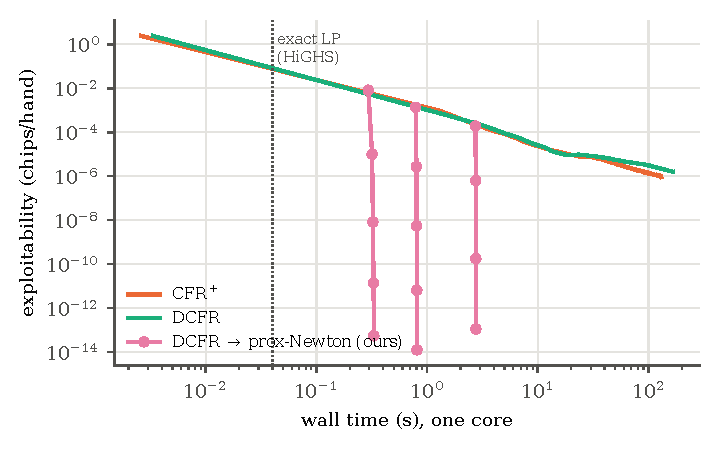
\includegraphics[width=\linewidth]{hybrid_leduc.pdf}
\column{0.38\textwidth}
Each pink curve starts where a short DCFR run stopped and drops straight down to machine precision.

\medskip
From \SuppLeducWarm\ DCFR iterations our method reaches $\SuppLeducExpl$ in \alert{\SuppLeducTime\
seconds}. CFR$^+$ is at $\LeducCFRplusLong$ after \LeducCFRplusLongTime\ seconds.

\medskip
Leduc is tiny and an LP solver needs 0.04 seconds. What matters is the shape of the curves.
\end{columns}
\note{
Each pink curve starts where the DCFR warm start stopped, after 100, 300 or 1000 iterations. The points are verification rounds.
Starting from 100 DCFR iterations is enough and costs one extra round. Starting later only costs DCFR time. The run used \SuppLeducRounds\ rounds and \SuppLeducSolves\ linear solves.\\[3pt]
The value of the game that we obtain, $-0.085606424078\ldots$ chips for the first player, agrees with the LP in all printed digits.\\[3pt]
Be upfront about the LP. Leduc has 964 unknowns and a simplex method finishes in 40 ms. The question is what happens when
the LP does not fit, which is the next slide.
}
\end{frame}

% =====================================================================================
\begin{frame}{\tagO\ Result on the river from the demonstration}
\begin{columns}[T]
\column{0.52\textwidth}
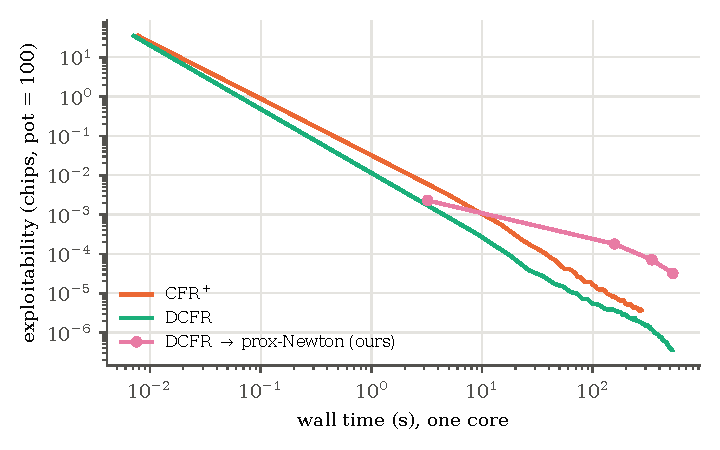
\includegraphics[width=\linewidth]{hybrid_medium.pdf}\\
{\scriptsize 473 against 328 hands and 17{,}626 unknowns. The points are verification rounds.}
\column{0.46\textwidth}
Our method runs DCFR for \SuppMedWarm\ iterations and then needs \SuppMedRounds\ rounds on a problem with \SuppMedFrac\%
of the unknowns. It reaches \alert{$\SuppMedExpl$ chips in \SuppMedTime\ seconds}.

\medskip
At that moment DCFR alone is at $\MedDCFRAtSuppTime$, and after \MedDCFRLongTwoIters\ iterations and \MedDCFRLongTwoTime\
seconds it is at $\MedDCFRLongTwoExpl$.

\medskip
Without the restriction to the support the Newton finish \emph{loses} to DCFR on this hand. The LP solver did not finish in 25
minutes.
\end{columns}
\note{
This is the slide that took the longest to earn. The first version of the method, Newton on the full sequence-form problem, worked
on Leduc and the small river and lost to DCFR here, with $\MedHybExpl$ after \MedHybTime\ seconds. The crossover from the interior point kept landing on a wrong active set,
because the equilibrium set is flat in directions that do not matter, and with
$\rho=10^{-5}$ an error in those directions is amplified by $1/\rho$. A larger $\rho$ made the active-set steps work and the
outer loop crawl. Anderson acceleration of the proximal map helped, to $8\times10^{-7}$ in 8 minutes, and then stalled.\\[3pt]
Restricting to the support predicted by CFR and verifying afterwards removes exactly those directions. \SuppMedAdded\ actions were added back in total.
Starting from 1{,}000 DCFR iterations gives $\SuppMedOneKExpl$ in \SuppMedOneKTime\ seconds.\\[3pt]
On the small river (147 against 139 hands) the method reaches $\SuppSmallExpl$ in \SuppSmallTime\ seconds, DCFR is at $\SmallDCFRExpl$ after \SmallDCFRTime\ seconds, and the LP takes 1.6 seconds. This is on a backup slide.
}
\end{frame}

% =====================================================================================
\begin{frame}{\tagO\ Where it stops winning, and what is open}
\begin{block}{Full ranges: all 1{,}081 hands for both players, 47{,}568 unknowns}
\small The restricted problem still has 43\% of the unknowns and one factorisation takes about 10 seconds. After 80 minutes our
method is at $4.1\times10^{-6}$ chips. DCFR reaches $9.5\times10^{-6}$ in 10 minutes. \textbf{Here CFR wins.}
\end{block}

\medskip
The bottleneck is the linear algebra. Each payoff block is dense, but it is a sorted sign matrix plus a sparse correction,
and a product with it costs $O(n\log n)$. A Newton--Krylov step would then cost only a few CFR iterations, provided we can
find a good preconditioner for systems of the form ``diagonal plus skew''. We think this is the most promising open problem,
and it is a problem in numerical linear algebra.

\medskip
Two further directions are a better prediction of the support from the CFR regrets, which would save verification rounds,
and the use of exact solves inside programs that play in real time.
\note{
The run with full ranges is the honest boundary of the method as implemented. The restriction still removes more than half of the
unknowns, but each factorisation of the remaining system with 20{,}000 unknowns takes about 10 seconds because the payoff blocks between
the hands that remain in play are dense. The first round needed 201 solves and 50 minutes, the second 116, and the second did not
reach machine precision (the proximal loop stalled at a residual of $5\times10^{-7}$).
DCFR does 40{,}000 iterations in 10 minutes.\\[3pt]
The research directions are natural ones for this club. The first is the one I would bet on: the structure that
makes CFR fast (sorting, running sums, card-removal corrections) is exactly the structure that a fast direct or preconditioned iterative
solver for the Newton systems would need. Hierarchical factorisations of the blocks are a candidate.
}
\end{frame}

% =====================================================================================
\begin{frame}{\tagO\ What is new here, and what is not}
The ingredients are classical: the sequence form, the proximal point method, semismooth Newton,
interior point with crossover, quasi-definite factorisations and the CFR family.

\medskip
The closest work is by Yang, Gao, Lin and Kroer (2025), who use a semismooth Newton method for \emph{matrix} games after a
first-order warm start.

\medskip
What we add is a second-order finish that works directly on the sequence form of a poker game. It has four parts:
\begin{itemize}\setlength\itemsep{0pt}
\item the skew formulation with a proximal term, which gives nonsingular Newton matrices by a one-line proof,
\item a warm start for both the strategies and the values taken from CFR,
\item the restriction to the support predicted by CFR, which removes the flat directions,
\item and the verification by exact best responses in the full game.
\end{itemize}
\note{
Be precise about novelty. The general idea of a first-order warm start followed by semismooth Newton for zero-sum games was proposed
for matrix games by Yang, Gao, Lin and Kroer in December 2025 (arXiv 2512.12910). Their Newton system lives on the normal form, they use
Douglas-Rachford splitting and a PRM$^+$ warm start, and they do not treat the structure of extensive-form games.\\[3pt]
To our knowledge no solver based on CFR hands over to a second-order method for the last digits. Early work solved small abstracted games exactly as linear programs (Gilpin and Sandholm 2005). The commercial and research poker solvers that we know of
(PioSolver, GTO+, Libratus, DeepStack) are first-order.
}
\end{frame}

% =====================================================================================
\begin{frame}{Takeaways}
A poker equilibrium is the solution of a structured saddle-point problem, and the sequence form turns it into a linear program
whose size is linear in the game tree.

\medskip
CFR is regret matching at every information set. It never forms the matrix, its proven rate is $T^{-1/2}$, and its modern
variants are much faster in practice, as the race in the browser showed.

\medskip
The output is readable poker: value bets, bluffs, traps and a defence that follows the pot odds.

\medskip
Read as a skew variational inequality, the same problem can be finished by a proximal Newton method. The obstacle is the
flatness of the equilibrium set, and restricting to the support that CFR predicts removes it. On our river this gives
an exploitability of $10^{-12}$ in about two minutes, where DCFR alone is at $10^{-6}$. With full ranges the linear algebra becomes the
bottleneck and CFR wins again.

\medskip
{\small The solver, the interactive page, the benchmarks and these slides are at \texttt{github.com/dwangnumbers/Poker-Solver}.}
\note{
End with the invitation. The open problem on the earlier slide is a natural one for this club: a preconditioner for
shifted skew systems whose off-diagonal blocks are a sorted sign matrix plus a sparse correction.\\[3pt]
If there is time left, go back to the browser and take requests: another board, another range, other bet sizes.
}
\end{frame}

% =====================================================================================
\begin{frame}{Main references}
\footnotesize
\begin{itemize}\setlength\itemsep{1pt}
\item D.~Koller, N.~Megiddo, B.~von Stengel. Efficient computation of equilibria for extensive two-person games. \emph{Games Econ.\ Behav.} 14 (1996).
\item M.~Zinkevich, M.~Johanson, M.~Bowling, C.~Piccione. Regret minimization in games with incomplete information. \emph{NeurIPS} 2007.
\item N.~Brown, T.~Sandholm. Solving imperfect-information games via discounted regret minimization. \emph{AAAI} 2019.
\item R.~T. Rockafellar. Monotone operators and the proximal point algorithm. \emph{SIAM J.\ Control Optim.} 14 (1976).
\item M.~Hinterm\"uller, K.~Ito, K.~Kunisch. The primal-dual active set strategy as a semismooth Newton method. \emph{SIAM J.\ Optim.} 13 (2002).
\item R.~J. Vanderbei. Symmetric quasidefinite matrices. \emph{SIAM J.\ Optim.} 5 (1995).
\item D.~Yang, Y.~Gao, T.~Lin, C.~Kroer. A direct second-order method for solving two-player zero-sum games. arXiv:2512.12910 (2025).
\end{itemize}
The complete list of references is in \texttt{talk-detailed.pdf}.
\end{frame}

% =====================================================================================
\appendix
\begin{frame}{Backup: Kuhn poker, where the equilibrium is not unique}
\begin{columns}[T]
\column{0.55\textwidth}
Kuhn poker uses the three cards \pcard[0.8]{J}{s}\,\pcard[0.8]{Q}{s}\,\pcard[0.8]{K}{s}. Each player puts in one chip and gets one card, and
there is a single bet of one chip.

\medskip
Its equilibria form a one-parameter family. The first player bets the jack as a bluff with any probability
$\alpha$ between 0 and $\tfrac13$, and bets the king with probability $3\alpha$. The value of the game is $-\tfrac1{18}$.

\medskip
The set of equilibria is a polytope and not a point, and any method has to cope with that.
\column{0.42\textwidth}
\begin{block}{Our computation}
\small
The Newton finish returns $\alpha = 0.198$ and bets the king with probability $0.593 = 3\alpha$.\\[2pt]
Value $-0.0555\ldots = -1/18$.\\[2pt]
Exploitability $1.1\times10^{-16}$.
\end{block}
\end{columns}
\note{Kuhn poker is the poker analogue of a two by two test matrix. Jacobians at a solution are
singular, and the proximal term picks one member of the family.}
\end{frame}

\begin{frame}{Backup: the first-order methods on Leduc hold'em}
\begin{columns}[c]
\column{0.58\textwidth}
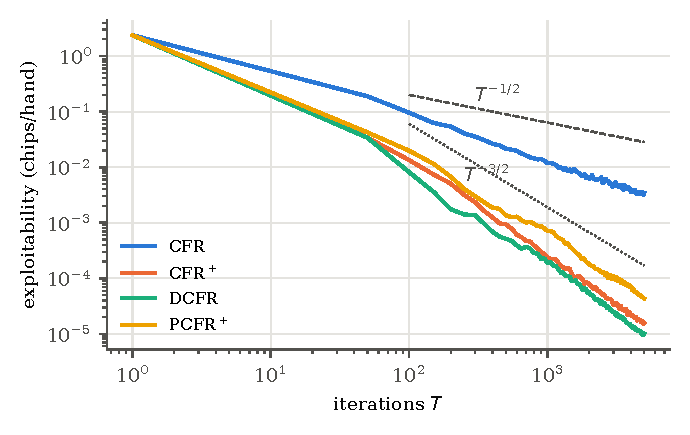
\includegraphics[width=\linewidth]{conv_leduc_iters.pdf}
\column{0.4\textwidth}
The curves show the exploitability of the average strategy for our implementation.

\medskip
After 5{,}000 iterations and \LeducDCFRfiveTime\ seconds DCFR reaches $\LeducDCFRfive$. After 50{,}000 iterations and
\LeducCFRplusLongTime\ seconds CFR$^+$ reaches $\LeducCFRplusLong$ and DCFR $\LeducDCFRLong$.

\medskip
Each extra digit costs about ten times more iterations.
\end{columns}
\note{Exploitability is in chips per hand, and the antes in Leduc are 1 chip.}
\end{frame}

\begin{frame}{Backup: a small river, and every linear solve of one exact solve}
\begin{columns}[c]
\column{0.5\textwidth}
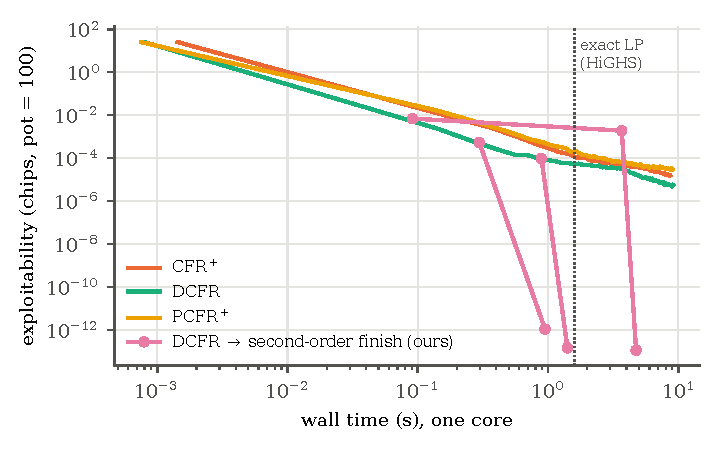
\includegraphics[width=\linewidth]{hybrid_small.pdf}
\column{0.48\textwidth}
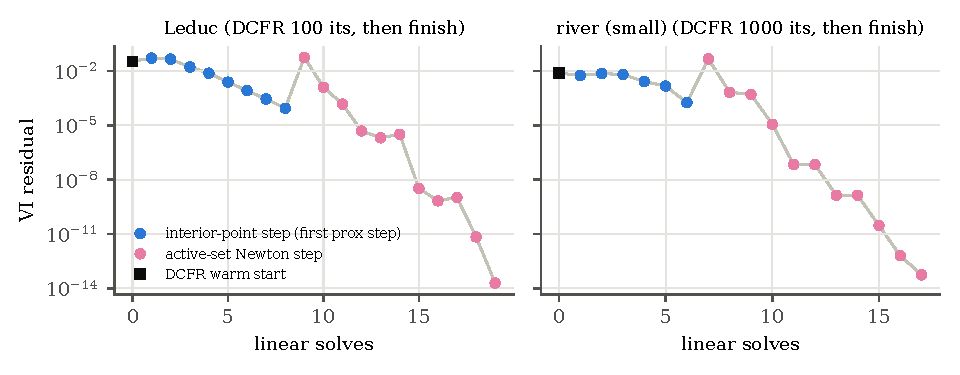
\includegraphics[width=\linewidth]{newton_inner.pdf}
\end{columns}
\medskip
\small On the left is a river with 147 against 139 hands. Our method reaches $\SuppSmallExpl$ chips in \SuppSmallTime\ seconds, DCFR is at
$\SmallDCFRExpl$ after \SmallDCFRTime\ seconds, and the LP takes 1.6 seconds. On the right is the residual after every linear solve. The blue
points are interior-point iterations and the pink points are Newton steps.
\note{The crossover lands on the exact solution of the first regularised
subproblem, whose residual is $\rho\|z^1-z^0\|$, hence the jump. After that each proximal step is solved exactly in one to three steps.}
\end{frame}

\begin{frame}{Backup: the rate of the proximal point method, and why flat equilibria hurt}
The proximal step is the resolvent of a maximal monotone operator $T$, so the iterates move monotonically towards the solution set $Z$.

\medskip
If $T^{-1}$ is upper Lipschitz at $0$ with modulus $a$, which holds for polyhedral problems, then
\[ \operatorname{dist}(z^{k+1}, Z) \ \le\ \frac{a\rho}{\sqrt{1 + a^2\rho^2}}\ \operatorname{dist}(z^k, Z). \]
The modulus $a$ measures how far a point with a small residual can be from $Z$. It is large when the equilibrium set is flat,
that is, when many hands have actions that barely matter.

\medskip
A fast outer loop needs $\rho$ much smaller than $1/a$. But $\|(M+\rho I)^{-1}\|\approx 1/\rho$ then makes the active set of each
subproblem fragile. On Leduc we observe a factor of about $10^{-3}$ for each step at $\rho=10^{-5}$. On the full river of the demonstration no
value of $\rho$ gave both, and the restriction to the support removes the flat directions instead.
\note{Backup for questions about the outer loop. Rockafellar 1976, Luque 1984, Robinson 1981.}
\end{frame}

\end{document}
"
%  This is the simplified deck that goes with the live demonstration (../app). The longer version is talk-detailed.tex.
%  Every number marked "we computed" comes from ../solver (see numbers.tex, generated by gen_numbers.py)
% =====================================================================================
\providecommand\notesmode{0}
\ifnum\notesmode=1 \PassOptionsToClass{handout}{beamer}\fi
\documentclass[10pt,aspectratio=169]{beamer}
\usetheme[progressbar=frametitle,numbering=fraction,block=fill]{metropolis}
\ifnum\notesmode=1
  \setbeameroption{show only notes}
\fi
\usepackage[T1]{fontenc}
\usepackage{lmodern}
\usepackage{amsmath,amssymb,mathtools}
\usepackage{booktabs}
\usepackage{xcolor}
\usepackage{tikz}
\usetikzlibrary{arrows.meta,positioning,calc,shapes.geometric,fit,backgrounds,decorations.pathreplacing}
\usepackage{graphicx}
\usepackage{fancyvrb}
\graphicspath{{../figs/}}
\newcommand{\LeducDCFRfive}{1.0\times 10^{-5}}
\newcommand{\LeducDCFRfiveTime}{14}
\newcommand{\LeducCFRplusLong}{9.2\times 10^{-7}}
\newcommand{\LeducCFRplusLongTime}{130}
\newcommand{\LeducDCFRLong}{1.6\times 10^{-6}}
\newcommand{\LeducHybWarm}{100}
\newcommand{\LeducHybTime}{0.33}
\newcommand{\LeducHybExpl}{5.5\times 10^{-14}}
\newcommand{\LeducHybOuter}{4}
\newcommand{\LeducHybNewton}{19}
\newcommand{\SmallDCFRTime}{9}
\newcommand{\SmallDCFRIters}{30{,}000}
\newcommand{\SmallDCFRExpl}{5.4\times 10^{-6}}
\newcommand{\SmallHybTime}{1.9}
\newcommand{\SmallHybExpl}{3.9\times 10^{-14}}
\newcommand{\SmallHybNewton}{17}
\newcommand{\SmallHybOuter}{6}
\newcommand{\MedDCFRTime}{16}
\newcommand{\MedDCFRExpl}{1.3\times 10^{-4}}
\newcommand{\MedDCFRIters}{5{,}000}
\newcommand{\MedHybTime}{528}
\newcommand{\MedHybExpl}{3.2\times 10^{-5}}
\newcommand{\MedHybOuter}{3}
\newcommand{\MedDCFRLongExpl}{1.8\times 10^{-6}}
\newcommand{\MedDCFRLongTime}{282}
\newcommand{\MedDCFRLongTwoExpl}{3.6\times 10^{-7}}
\newcommand{\MedDCFRLongTwoTime}{520}
\newcommand{\MedDCFRLongTwoIters}{190{,}000}
\newcommand{\MedCFRpLongExpl}{3.8\times 10^{-6}}
\newcommand{\LeducSolves}{19}
\newcommand{\LeducIPM}{8}
\newcommand{\LeducFinishTime}{0.04}
\newcommand{\LeducWarmTime}{0.29}
\newcommand{\SmallSolves}{17}
\newcommand{\SmallIPM}{6}
\newcommand{\SmallFinishTime}{1.58}
\newcommand{\SmallWarmTime}{0.30}
\newcommand{\LeducPure}{49}
\newcommand{\LeducSupport}{59}
\newcommand{\LeducN}{964}
\newcommand{\SmallPure}{71}
\newcommand{\SmallSupport}{52}
\newcommand{\SmallN}{2{,}864}
\newcommand{\SuppLeducTime}{0.30}
\newcommand{\SuppLeducExpl}{6.8\times 10^{-14}}
\newcommand{\SuppLeducRounds}{2}
\newcommand{\SuppLeducWarm}{100}
\newcommand{\SuppLeducSolves}{26}
\newcommand{\SuppSmallTime}{0.95}
\newcommand{\SuppSmallExpl}{1.1\times 10^{-12}}
\newcommand{\SuppSmallRounds}{1}
\newcommand{\SuppSmallWarm}{1{,}000}
\newcommand{\SuppSmallSolves}{16}
\newcommand{\SuppMedTime}{131}
\newcommand{\SuppMedExpl}{2.8\times 10^{-12}}
\newcommand{\SuppMedRounds}{3}
\newcommand{\SuppMedWarm}{3{,}000}
\newcommand{\SuppMedSolves}{163}
\newcommand{\SuppMedFrac}{34}
\newcommand{\SuppMedAdded}{16}
\newcommand{\MedDCFRAtSuppTime}{3.9\times 10^{-6}}
\newcommand{\MedDCFRAtSuppIters}{47{,}490}
\newcommand{\SuppMedOneKTime}{152}
\newcommand{\SuppMedOneKExpl}{3.8\times 10^{-12}}


% ---------- palette (validated categorical slots + inks) ----------
\definecolor{cblue}{HTML}{2A78D6}
\definecolor{corange}{HTML}{EB6834}
\definecolor{caqua}{HTML}{1BAF7A}
\definecolor{cyellow}{HTML}{EDA100}
\definecolor{cmagenta}{HTML}{E87BA4}
\definecolor{ink}{HTML}{0B0B0B}
\definecolor{ink2}{HTML}{52514E}
\definecolor{paper}{HTML}{FCFCFB}
\definecolor{lightblue}{HTML}{CDE2FB}
\definecolor{lightgray}{HTML}{E4E3DF}
\definecolor{felt}{HTML}{1F6B4A}
\definecolor{suitred}{HTML}{C8102E}
\definecolor{suitblue}{HTML}{1C5CAB}
\definecolor{suitgreen}{HTML}{147A3A}
\setbeamercolor{normal text}{fg=ink,bg=paper}
\setbeamercolor{alerted text}{fg=corange}
\setbeamercolor{progress bar}{fg=cblue,bg=lightgray}
\setbeamercolor{frametitle}{bg=ink,fg=paper}
\setbeamercolor{block title}{bg=lightblue,fg=ink}
\setbeamercolor{block body}{bg=lightblue!35,fg=ink}
\setbeamercolor{example text}{fg=caqua!80!black}
\metroset{titleformat frame=regular}
\setbeamerfont{note page}{size=\scriptsize}

% ---------- notation ----------
\newcommand{\src}[1]{{\par\vfill\hfill\tiny\color{ink2}#1}}
\newcommand{\R}{\mathbb{R}}
\newcommand{\ex}{\operatorname{expl}}
\newcommand{\tagP}{\tikz[baseline=-0.6ex]\node[fill=felt,text=white,rounded corners=1.5pt,inner sep=1.6pt,font=\tiny\bfseries]{POKER};}
\newcommand{\tagM}{\tikz[baseline=-0.6ex]\node[fill=cblue,text=white,rounded corners=1.5pt,inner sep=1.6pt,font=\tiny\bfseries]{MATH};}
\newcommand{\tagO}{\tikz[baseline=-0.6ex]\node[fill=corange,text=white,rounded corners=1.5pt,inner sep=1.6pt,font=\tiny\bfseries]{NEW};}

% ---------- playing cards (four-colour deck) ----------
\colorlet{suit-s}{ink}\colorlet{suit-h}{suitred}\colorlet{suit-d}{suitblue}\colorlet{suit-c}{suitgreen}
\newcommand{\suitsym}[1]{\ensuremath{\csname suit@#1\endcsname}}
\makeatletter
\def\suit@s{\spadesuit}\def\suit@h{\heartsuit}\def\suit@d{\diamondsuit}\def\suit@c{\clubsuit}
\makeatother
\newcommand{\pcard}[3][1]{% [scale]{rank}{suit}
  \tikz[baseline=-0.7ex]{\node[draw=ink2,fill=white,rounded corners=2.5pt,minimum width=#1*0.62cm,
  minimum height=#1*0.86cm,inner sep=0pt,text=suit-#3,font=\bfseries\sffamily]
  {\shortstack{#2\\[-1pt]\suitsym{#3}}};}}
\newcommand{\cardback}{\tikz[baseline=-0.7ex]{\node[draw=white,fill=suitred!80!black,rounded corners=2pt,
  minimum width=0.42cm,minimum height=0.6cm,inner sep=0pt]{};}}

\title{Solving Poker}
\subtitle{The numerical analysis behind poker solvers\\ --- and a second-order finish for them}
\author{Numerical Analysis Research Club}
\date{}

\begin{document}

% =====================================================================================
\begin{frame}
  \titlepage
\note{
\textbf{Timing plan for 60 minutes.} Opening and rules 5 $\cdot$ Games, equilibria and the linear program 9 $\cdot$
Regret minimisation and CFR 9 $\cdot$ Live demonstration 12 $\cdot$ The new method 13 $\cdot$ Results, limits and wrap-up 8.
That leaves about four minutes for questions during the talk.\\[4pt]
If running late, shorten the demonstration to its five minute version (see \texttt{app/DEMO\_NOTES.md}) and give the slide
``Making it robust and fast'' one sentence.\\[4pt]
Opening line: ``Ten years ago the best poker players in the world lost to programs whose core is a few lines of
arithmetic repeated a few billion times. This talk is about that arithmetic, read as numerical analysis, and about
what a numerical analyst can add to it.''\\[4pt]
The slides alternate between \textsc{poker} (green tag) and \textsc{math} (blue tag). The orange tag \textsc{new} marks
our own contribution. Every number that we computed comes from the Python solver in the repository. The more detailed
version of this deck, with all citations and extra slides, is \texttt{talk-detailed.pdf}.
}
\end{frame}

% =====================================================================================
\begin{frame}{\tagP\ Ten years of superhuman poker}
\begin{columns}[T]
\column{0.58\textwidth}
In 2015 a program called Cepheus essentially solved two-player limit hold'em.

\medskip
In 2017 two programs, DeepStack and Libratus, beat professional players at the no-limit game, which is far larger.
In 2019 Pluribus did the same at a table of six.

\medskip
Today every serious player studies with a \alert{solver}. You describe one situation, and the program computes how
to play every possible hand in it.

\medskip
All of these programs share one simple iteration. This talk explains it and then tries to improve on it.
\column{0.4\textwidth}
\centering
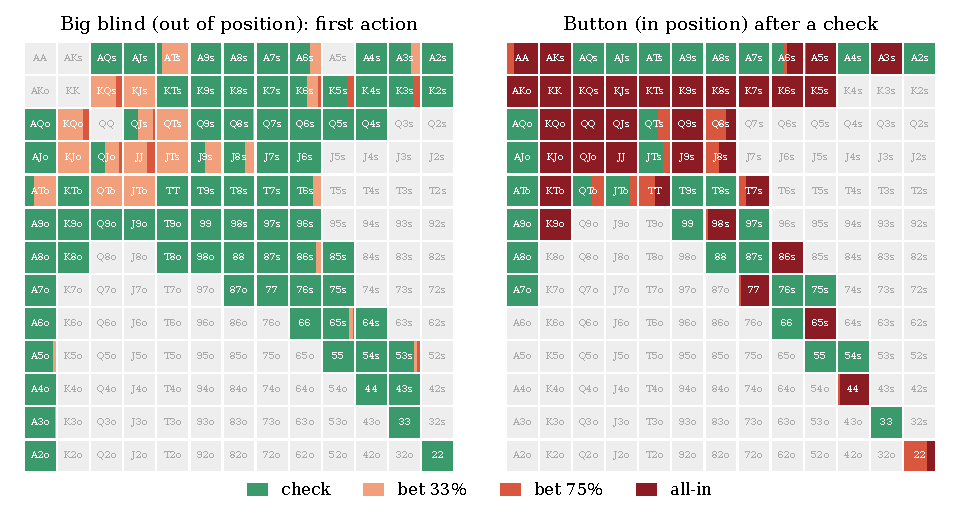
\includegraphics[height=0.6\textheight,trim=0 22 245 0,clip]{grid_root.pdf}\\[-2pt]
{\scriptsize\color{ink2} A solver's answer, computed by our own code. Each square is a starting hand and the colours are actions.}
\end{columns}
\note{
The common core of all these programs is an iterative method, counterfactual regret minimisation, applied to a very large
saddle-point problem. Libratus and DeepStack add abstraction (shrinking the game) and subgame solving
(solving again the part of the game you are actually in), but the inner loop is still a method of the CFR family.\\[3pt]
Commercial solvers such as PioSolver, GTO+ and GTO Wizard are what human players use. You give the board, the
two ranges and the allowed bet sizes, and the program computes an equilibrium of that subgame. The picture on the right is
exactly such an output, produced by our solver for the river situation that we use for the whole talk.\\[3pt]
References if asked: Bowling et al., Science 2015. Morav\v{c}\'ik et al., Science 2017. Brown and Sandholm, Science 2018 and 2019.
}
\end{frame}

% =====================================================================================
\begin{frame}{The plan: poker $\leftrightarrow$ math}
\centering
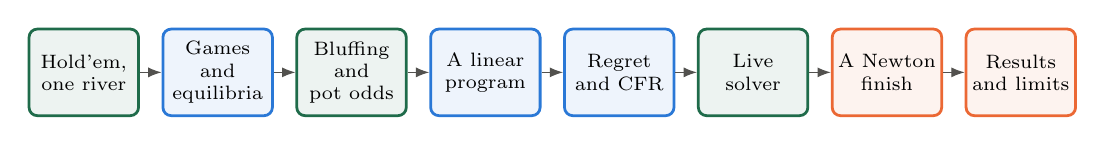
\begin{tikzpicture}[x=1cm,y=1cm,every node/.style={font=\scriptsize}]
  \foreach \i/\t/\c in {0/{Hold'em,\\ one river}/felt, 1/{Games and\\ equilibria}/cblue, 2/{Bluffing and\\ pot odds}/felt,
                       3/{A linear\\ program}/cblue, 4/{Regret\\ and CFR}/cblue, 5/{Live\\ solver}/felt,
                       6/{A Newton\\ finish}/corange, 7/{Results\\ and limits}/corange}{
    \node[draw=\c,line width=1pt,rounded corners=3pt,text width=1.25cm,minimum height=1.1cm,align=center,
          inner sep=2pt,fill=\c!8] (n\i) at (1.7*\i,0) {\t};
  }
  \foreach \i [evaluate=\i as \j using int(\i+1)] in {0,...,6} { \draw[-{Latex},ink2] (n\i) -- (n\j); }
\end{tikzpicture}

\vspace{1.4em}
\raggedright
The equilibrium of a poker game is the solution of a very large and very structured saddle-point problem.
Solvers attack it with a first-order method whose steps are cheap and whose last digits are slow.

\medskip
In the middle of the talk we solve a real hand live in the browser and look at the answer together.

\medskip
Our own contribution comes last. We treat the end of the solve as a nonsmooth equation and finish it with a Newton
method, which reaches machine precision where the first-order method would need millions of iterations.
\note{
Say what the audience will get. First, enough poker to read the output of a solver. Second, the mathematics of why CFR converges
and why it is fast in practice. Third, a live demonstration in which they can ask for any change to the hand. Fourth, a new method
from the numerical optimisation toolbox, with honest results: where it wins by orders of magnitude, and where it does not yet.
}
\end{frame}

% =====================================================================================
\begin{frame}{\tagP\ Texas hold'em in one slide}
\begin{columns}[T]
\column{0.5\textwidth}
Each of the two players is dealt two private cards. Five public cards, the \emph{board}, are then revealed in three
stages called the flop, the turn and the river.

\medskip
There is a round of betting before the flop and after each stage. A player may check, bet, call, raise or fold, and in the
no-limit game a bet can be any size up to the player's stack.

\medskip
If nobody folds, the best five-card hand made from the seven available cards wins the pot.
\column{0.48\textwidth}
\centering
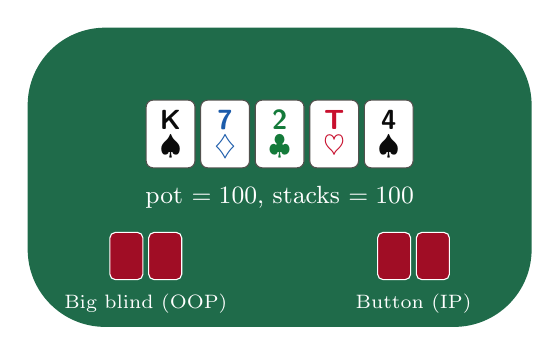
\begin{tikzpicture}
  \fill[felt,rounded corners=28pt] (-3.2,-1.9) rectangle (3.2,1.9);
  \node at (0,0.55) {\pcard{K}{s}\,\pcard{7}{d}\,\pcard{2}{c}\,\pcard{T}{h}\,\pcard{4}{s}};
  \node[text=white,font=\small] at (0,-0.25) {pot $= 100$, stacks $= 100$};
  \node at (-1.7,-1.0) {\cardback\,\cardback};
  \node at (1.7,-1.0) {\cardback\,\cardback};
  \node[text=white,font=\scriptsize] at (-1.7,-1.6) {Big blind (OOP)};
  \node[text=white,font=\scriptsize] at (1.7,-1.6) {Button (IP)};
\end{tikzpicture}\\[4pt]
{\small Our running example is the \alert{river}, the last round of betting.\\
The big blind acts first, which is called being out of position.}
\end{columns}
\note{
Keep this light, since most of the audience has played or watched poker. The key structural fact is that the board is
public and the two hole cards are private. A strategy must therefore be a function of
the public history and your own cards. You do not know the opponent's cards, only a probability distribution over them,
which poker players call a \textbf{range}.\\[3pt]
The river situation is fixed for the whole talk: board K$\spadesuit$ 7$\diamondsuit$ 2$\clubsuit$ T$\heartsuit$ 4$\spadesuit$, pot 100, both players
have 100 behind. The big blind may check or bet 33\% or 75\% of the pot or go all-in. Facing a bet you may fold, call or go all-in.
The live demonstration uses exactly this table.
}
\end{frame}

% =====================================================================================
\begin{frame}{\tagP\ Ranges: what a solver takes as input}
\begin{columns}[T]
\column{0.6\textwidth}
\centering
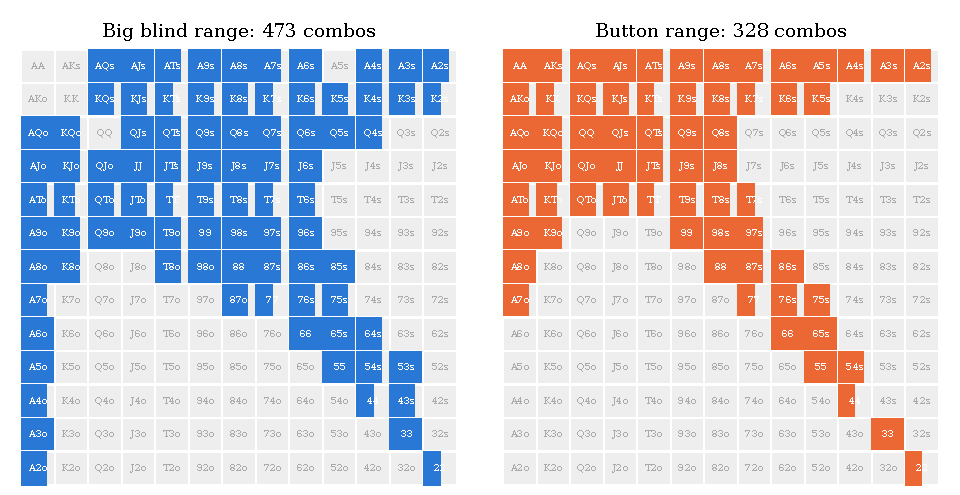
\includegraphics[width=\linewidth]{ranges.pdf}
\column{0.38\textwidth}
A \textbf{range} is a probability vector over the two-card hands a player can hold. There are 1326 such hands, and 1081
once the five board cards are known.

\medskip
In our example the big blind called a raise before the flop and the button made that raise, so the two ranges are
different.

\medskip
The solver returns, for every point of the betting and for every hand, a probability for each action.
\end{columns}
\note{
The 13 by 13 grid is the standard poker picture. Pairs are on the diagonal, suited hands above it and offsuit hands below it.
Each cell is a class of hands, for example AKs stands for 4 combinations. Mathematically the input is two nonnegative vectors
$r_1\in\R^{n_1}$ and $r_2\in\R^{n_2}$. Two hands that share a card cannot both be dealt, which is called card removal, and it is a 0/1
compatibility matrix $C$ between the ranges. Both will appear in the formulas later.\\[3pt]
The width of each bar shows how many combinations are still possible given the board. The king of spades is on the board, so there
are fewer hands with a king.
}
\end{frame}

% =====================================================================================
\begin{frame}{\tagM\ Two-player zero-sum games and Nash equilibrium}
Each player chooses a strategy from a compact convex set, $x\in X$ and $y\in Y$, and the first player receives the
bilinear payoff $x^\top A y$ from the second.
\begin{block}{Minimax theorem (von Neumann 1928)}
\[ \max_{x\in X}\min_{y\in Y} x^\top A y \;=\; \min_{y\in Y}\max_{x\in X} x^\top A y \;=:\; v^\ast . \]
\end{block}
A pair $(x^\ast,y^\ast)$ that attains both sides is a \textbf{Nash equilibrium}, and $v^\ast$ is the value of the game.
Playing $x^\ast$ guarantees at least $v^\ast$ against any opponent, which is what poker players mean by an unexploitable strategy.
\begin{block}{The error that every solver reports is the exploitability}
\[\ex(x,y) \;=\; \tfrac12\Big(\max_{x'} x'^\top A y \;-\; \min_{y'} x^\top A y'\Big)\;\ge 0 ,
  \qquad\text{with equality exactly at an equilibrium.}\]
\end{block}
\note{
For an applied mathematics audience this is a convex-concave saddle-point problem with a bilinear coupling, and the exploitability
is the primal-dual gap. Everything later is a method for driving this gap to zero. Its unit is chips per hand.\\[3pt]
Practical solvers stop at an exploitability of a fraction of a percent of the pot. We will push to $10^{-13}$.
Our numbers are in chips with a pot of 100, so $10^{-2}$ chips is $10^{-4}$ of the pot.
}
\end{frame}

% =====================================================================================
\begin{frame}{\tagP\ Why equilibria mix: bluffing and pot odds}
\begin{columns}[T]
\column{0.56\textwidth}
Take a toy river with a pot of 1. The bettor holds either the best hand or nothing and bets $s$. The caller holds a
medium hand that only beats a bluff.

\medskip
The caller is indifferent between calling and folding when bluffs are a fraction $\beta = \dfrac{s}{1+2s}$ of the bets.

\medskip
The bettor's bluffs are indifferent when the caller continues with probability $\dfrac{1}{1+s}$. Poker players call
this the \emph{minimum defence frequency}.

\medskip
Any pure strategy can be exploited here. The equilibrium randomises, and it does so exactly where the opponent
is made indifferent.
\column{0.4\textwidth}
\centering
\begin{tabular}{ccc}
\toprule
bet $s$ & bluffs $\beta$ & defend \\ \midrule
$1/3$ & 20\% & 75\% \\
$3/4$ & 30\% & 57\% \\
$1$ & 33\% & 50\% \\
$2$ & 40\% & 33\% \\ \bottomrule
\end{tabular}\\[10pt]
{\small We will check the last column against the live solver.}
\end{columns}
\note{
Derivation, to say and not to write. For the caller, calling wins $1+s$ against a bluff and loses $s$ against a value bet.
The caller is indifferent when $\beta(1+s) = (1-\beta)s$, which gives $\beta = s/(1+2s)$. For the bettor with nothing, betting wins the pot $1$
when the caller folds and loses $s$ when called, and checking wins nothing. The bettor is indifferent when $(1-c)\cdot 1 = c\, s$, which gives $c = 1/(1+s)$.\\[3pt]
The mathematical point: at an equilibrium every action played with positive probability is a best response. This is
complementary slackness in the linear program that we are about to write down. Mixing happens exactly where reduced costs vanish.
}
\end{frame}

% =====================================================================================
\begin{frame}{\tagM\ Games on trees with hidden information}
\begin{columns}[T]
\column{0.52\textwidth}
Poker is a game tree. Chance deals the cards, the players act in turn, and the leaves carry the payoffs.

\medskip
A player cannot see the opponent's cards, so several nodes look the same to that player. Such a group of
nodes is an \textbf{information set}, and a strategy assigns a probability distribution over actions to each one.

\medskip
{\footnotesize
\begin{tabular}{lr}
\toprule
game & information sets \\ \midrule
Kuhn poker & 12 \\
Leduc hold'em & 288 \\
Limit hold'em & $3.2\times10^{14}$ \\
No-limit hold'em & about $10^{161}$ \\ \bottomrule
\end{tabular}}
\column{0.46\textwidth}
\centering
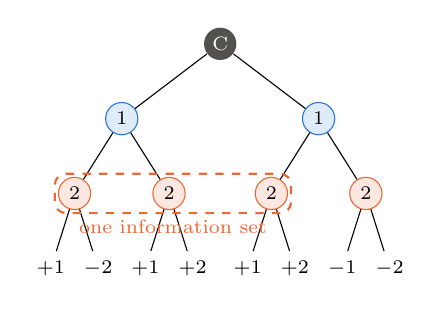
\begin{tikzpicture}[level distance=0.95cm,
   level 1/.style={sibling distance=2.5cm},level 2/.style={sibling distance=1.2cm},level 3/.style={sibling distance=0.6cm},
   every node/.style={font=\scriptsize}]
  \node[circle,fill=ink2,text=white,inner sep=1.5pt] {C}
    child { node[circle,draw=cblue,fill=cblue!15,inner sep=2pt] (a) {1}
       child { node[circle,draw=corange,fill=corange!15,inner sep=2pt] (b1) {2} child{node{$+1$}} child{node{$-2$}} }
       child { node[circle,draw=corange,fill=corange!15,inner sep=2pt] (b2) {2} child{node{$+1$}} child{node{$+2$}} } }
    child { node[circle,draw=cblue,fill=cblue!15,inner sep=2pt] (c) {1}
       child { node[circle,draw=corange,fill=corange!15,inner sep=2pt] (d1) {2} child{node{$+1$}} child{node{$+2$}} }
       child { node[circle,draw=corange,fill=corange!15,inner sep=2pt] (d2) {2} child{node{$-1$}} child{node{$-2$}} } };
  \draw[corange,dashed,thick,rounded corners] ($(b1)+(-0.25,0.25)$) -- ($(d1)+(0.25,0.25)$) -- ($(d1)+(0.25,-0.25)$) -- ($(b1)+(-0.25,-0.25)$) -- cycle;
  \node[corange,font=\scriptsize] at ($(b1)!0.5!(d1)+(0,-0.42)$) {one information set};
\end{tikzpicture}\\[2pt]
{\scriptsize Player 2 sees the action of player 1 but not the deal.}
\end{columns}
\note{
Leduc hold'em is the standard research benchmark. It has a deck of six cards, one private
card each, one public card, and two betting rounds. It has 288 information sets and we use it as our small test problem.\\[3pt]
The size column is the reason the subject exists. Nobody can write down no-limit hold'em. Real systems solve an abstraction
in which similar hands and bet sizes are merged, and then solve subgames like our river again during play.\\[3pt]
We assume perfect recall: a player never forgets what he knew or did. Sizes are from Bowling et al.\ 2015 and Johanson 2013.
Kuhn and Leduc were counted by our code.
}
\end{frame}

% =====================================================================================
\begin{frame}{\tagM\ The sequence form: equilibrium is a linear program}
Give player 1 one variable $x_\sigma$ for each \emph{sequence} $\sigma$ of her own
actions, equal to the product of her probabilities along it. These variables satisfy linear flow constraints
$Ex = e$, $x\ge 0$, and the expected payoff is bilinear in them, $u(x,y) = x^\top A y$.
\begin{block}{Theorem (Koller, Megiddo and von Stengel 1996)}
An equilibrium strategy of player 1 solves
\[\max_{x,\,q}\ f^\top q\quad \text{subject to}\quad A^\top x - F^\top q \ge 0,\quad Ex = e,\quad x\ge 0 ,\]
a linear program whose size is \emph{linear} in the size of the game tree.
\end{block}
So why not call an LP solver? On our river $A$ has 2.9 million nonzeros, because every leaf couples every hand of one
player to every hand of the other, and a good LP code did not finish in 25 minutes. The iteration we describe next
reaches $\MedDCFRExpl$ chips in \MedDCFRTime\ seconds.
\note{
This is the key modelling step. Mixed strategies over the pure strategies of the normal form would have exponentially many
variables. Realisation plans have one variable per sequence, and perfect recall makes the payoff bilinear in them.\\[3pt]
$E$ and $F$ are very sparse, with one row per information set and entries $\pm1$, and they encode flow conservation on a tree.
$A$ is where the poker lives. The program has 17{,}626 unknowns on our river. Say that the dual variables $q$ are the values of the opponent's information sets, and remember them: they are values of information sets, the same quantities
that CFR computes in every iteration. This is how we will warm-start the duals later.\\[3pt]
The LP run used HiGHS through SciPy with default settings on one core and we stopped it after 25 minutes. On the smaller test
problems the LP is perfectly fine: 0.04 s on Leduc and 1.6 s on a small river. The DCFR figure is for \MedDCFRIters\ iterations.
}
\end{frame}

% =====================================================================================
\begin{frame}{\tagM\ Regret matching}
\begin{columns}[T]
\column{0.62\textwidth}
We face the same decision many times. The \emph{regret} $R_T(a)$ of an action is how much better it would have done
than what we played. Regret matching plays each action in proportion to its positive regret.
{\small\[ R_T(a) = \sum_{t=1}^T \big(u_t(a) - u_t(\sigma_t)\big),\quad
   \sigma_{T+1}(a) = \frac{[R_T(a)]^+}{\sum_b [R_T(b)]^+}. \]}
\begin{block}{Theorem (Hart and Mas-Colell 2000)}
The regrets grow only like $\sqrt{T}$: $\ \max_a R_T(a) \le \Delta\sqrt{|A|\,T}$.
\end{block}
When both players of a zero-sum game do this, their \emph{average} strategies converge to an equilibrium.
\column{0.36\textwidth}
\centering
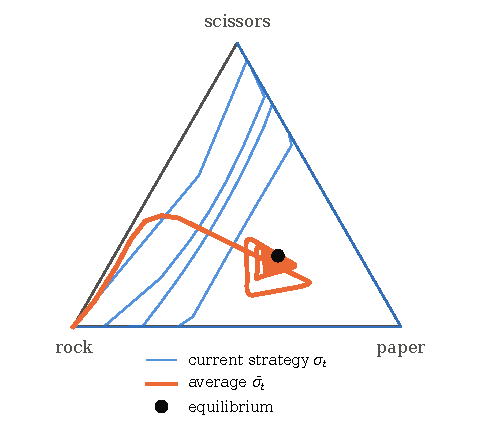
\includegraphics[width=\linewidth]{rm_rps.pdf}\\
{\scriptsize Our computation on a weighted rock-paper-scissors game. The current strategy cycles and the average converges.}
\end{columns}
\note{
Idea of the proof. The regret vector satisfies $\|[R_{T}]^+\|^2 \le \|[R_{T-1}]^+\|^2 + \Delta^2|A|$ because the
cross term $\langle [R_{T-1}]^+, r_T\rangle$ vanishes by the choice of $\sigma_T$: the instantaneous regret is orthogonal to the
current positive regrets. Sum and take square roots. This is Blackwell approachability, and $\Delta$ is the range of the payoffs.\\[3pt]
The folk theorem: if both players have average regret at most $\varepsilon$ then the average strategies are a $2\varepsilon$-equilibrium,
because $\max_{x'} x'^\top A \bar y - \min_{y'} \bar x^\top A y' \le 2\varepsilon$.\\[3pt]
In the figure the limit is $(\frac14,\frac12,\frac14)$.
}
\end{frame}

% =====================================================================================
\begin{frame}{\tagM\ Counterfactual regret minimisation (CFR)}
CFR runs regret matching separately at every information set $I$. The payoff it feeds to each one is the
\textbf{counterfactual value} of an action, which is the expected payoff weighted by the probability that the opponent and
chance lead to $I$, as if the player herself had tried to get there.
\[ v_i(\sigma, I, a) = \sum_{h\in I}\ \pi_{-i}^{\sigma}(h)\sum_{z \sqsupset ha} \pi^{\sigma}(ha\to z)\, u_i(z) \]
\begin{block}{Theorem (Zinkevich, Johanson, Bowling and Piccione 2007)}
The regret of the whole strategy is at most the sum of the local regrets. Therefore the average strategies satisfy
\[ \ex(\bar x_T,\bar y_T) \ \le\ \frac{\Delta\,|\mathcal I|\sqrt{|A|}}{\sqrt T}. \]
\end{block}
One iteration is one pass over the tree, with reach probabilities computed on the way down and values on the way up.
The matrix $A$ is never formed.
\note{
The decomposition is the whole trick. A global regret over an exponentially large strategy space is bounded by a sum of small
local regrets, and each of them is minimised by plain regret matching. This is why CFR scales: the cost of an iteration is linear in the tree
and so is the storage, two numbers for each information set and action.\\[3pt]
In the language of linear algebra, one CFR iteration computes $Ay$ and $A^\top x$ for the current realisation plans by walking the tree.
These are the same two products that any first-order saddle-point method needs.
}
\end{frame}

% =====================================================================================
\begin{frame}{\tagP\tagM\ CFR for poker: one pass for all hands}
In poker the betting is public and only the cards are hidden. At each point of the betting we store
\emph{vectors} indexed by hands, such as the reach probabilities $\pi_1$ and $\pi_2$.
At a leaf the values of all hands come from one matrix-vector product.
\[ v_1 = \text{amount}\cdot B\,\pi_2,\qquad
   B_{ij} = \underbrace{C_{ij}}_{\text{no shared card}}\cdot\begin{cases} 1 & \text{after a fold}\\ \operatorname{sign}(s_i - s_j) & \text{at a showdown}\end{cases} \]
Here $s_i$ is the strength of hand $i$. The matrix $B$ is dense but very structured. Once the hands are sorted by
strength, the sign matrix is all ones below the diagonal and all minus ones above it, and $C$ is the all-ones matrix
minus a sparse correction for hands that share a card.

\medskip
As a result $B\pi$ costs one sort and a running sum, which is $O(n\log n)$ operations and not $n^2$.
\note{
This is the bridge between the tree picture and the implementation. The information sets at a public node are indexed by the
private hand of the player to act, so all information sets at this node form a vector and every CFR operation becomes a vector operation.\\[3pt]
This is also the poker-specific numerical linear algebra. Each terminal block is low rank plus sparse. The fold block is
rank one minus a sparse correction. The showdown block, after sorting, is a sign matrix, which is semiseparable (think of the inverse of
a bidiagonal matrix), times the compatibility mask. The trick is due to Johanson et al.\ 2011.\\[3pt]
The public tree itself is drawn live in the demonstration, so it is not on a slide any more. It has 12 decision points and 21 leaves, and one iteration takes about a millisecond in the browser. Keep in mind that this structure is what a
scalable Newton method would have to exploit, which comes back at the end of the talk.
}
\end{frame}

% =====================================================================================
\begin{frame}{\tagM\ Four variants of one loop}
Modern solvers change how CFR weights the old regrets and how it averages the strategies.

\smallskip
\renewcommand{\arraystretch}{1.15}\small
\begin{tabular}{p{1.5cm}p{6.4cm}p{5.0cm}}
\toprule
method & what changes & a numerical analyst would say \\ \midrule
CFR$^+$ & Negative regrets are reset to zero and later strategies get more weight in the average. & projection onto the nonnegative orthant \\
DCFR & Old regrets and old strategies are multiplied by factors below one. & forgetting factors that damp the transient \\
PCFR$^+$ & The strategy is computed from the regrets plus a prediction of the next regret. & optimism, as in the extragradient method \\ \bottomrule
\end{tabular}

\smallskip
\normalsize The proven rate is still $T^{-1/2}$ for all four. In practice the modern variants are much faster, and we will
now race them against each other on a real hand.
\note{
CFR$^+$ (Tammelin 2014) is what solved limit hold'em. DCFR (Brown and Sandholm 2019) with parameters $(1.5, 0, 2)$ is the default in many solvers:
positive regrets are multiplied by $t^{1.5}/(t^{1.5}+1)$, negative ones by $1/2$, and the average by $(t/(t+1))^2$.
PCFR$^+$ (Farina, Kroer and Sandholm 2021) uses the last instantaneous regret as its prediction and connects regret matching to optimistic mirror descent.\\[3pt]
All four also update the two players in turn, so that the second player already sees the new strategy of the first, which is Gauss-Seidel in place of Jacobi.\\[3pt]
The observed rates are between $T^{-1}$ and $T^{-3/2}$ for the averages, while the last iterate oscillates. Explaining this gap to the
theory is an open question. The rates are still sublinear, and that is the gap our method addresses.
}
\end{frame}

% =====================================================================================
\begin{frame}{\tagP\tagM\ Live demonstration: the river solver table}
\begin{columns}[c]
\column{0.55\textwidth}
\centering
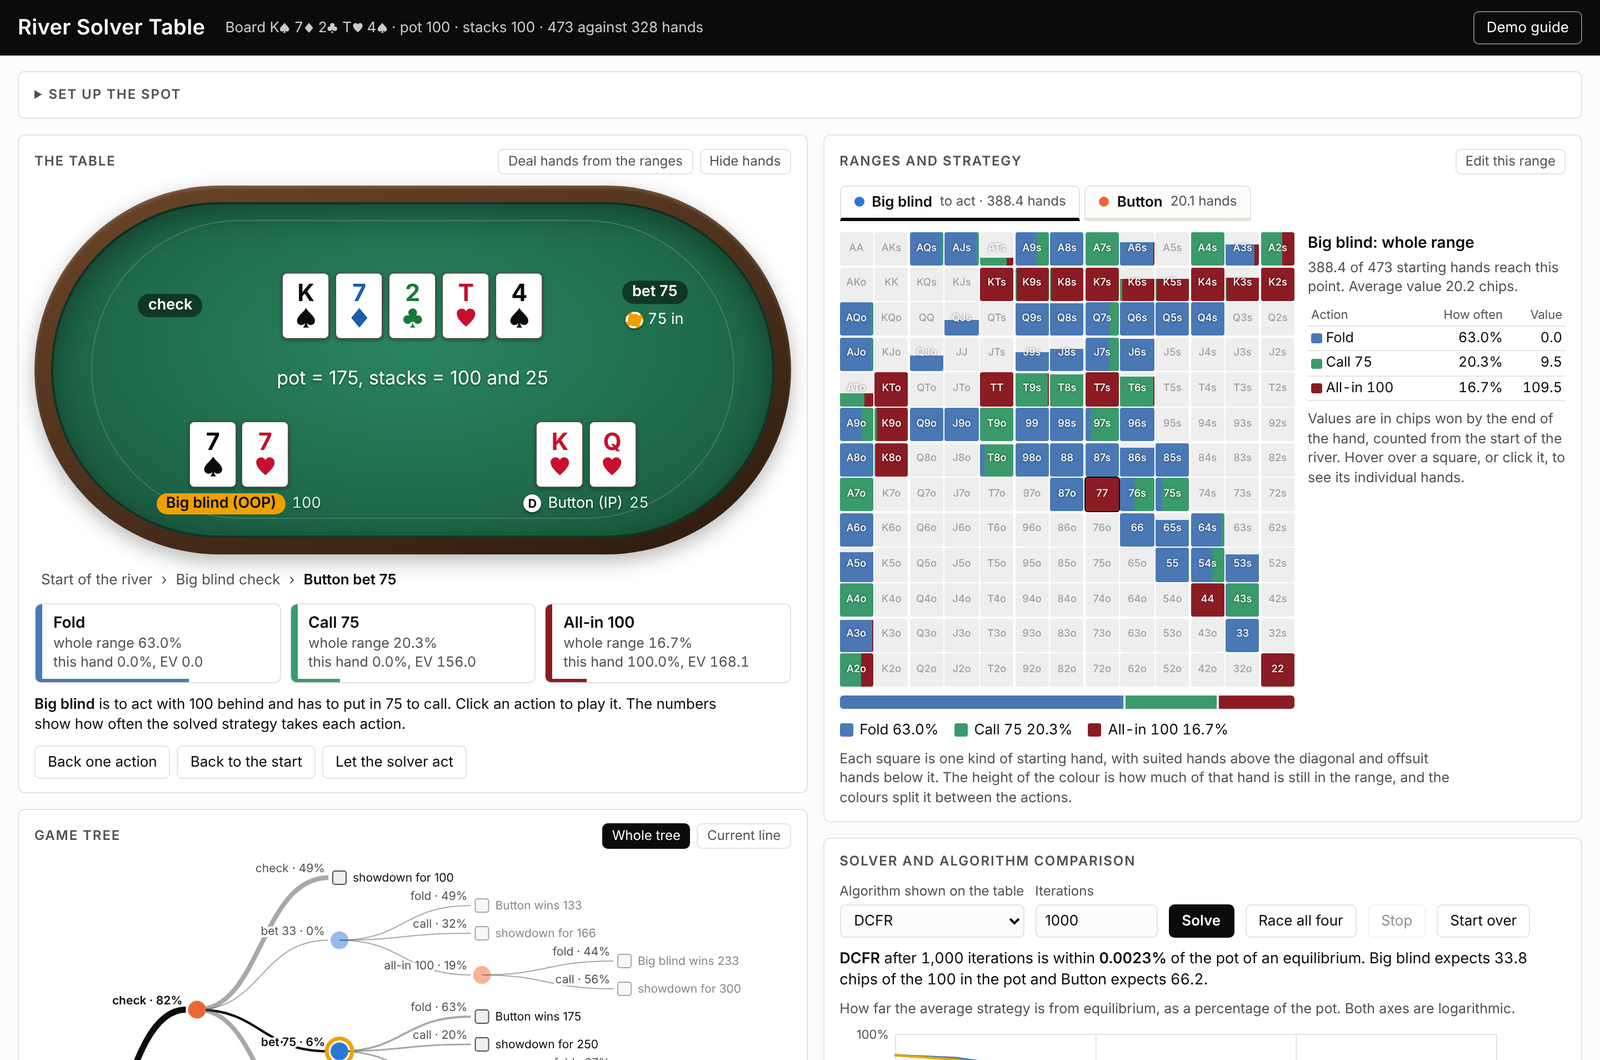
\includegraphics[width=\linewidth]{app_slide.png}
\column{0.43\textwidth}
The page \texttt{app/poker-solver.html} solves our river in the browser. It will answer five questions.
\begin{enumerate}\small\setlength\itemsep{2pt}
\item Which of the four algorithms wins a race?
\item What does the big blind do with each of its 473 hands?
\item How do the ranges and the tree change as the hand is played?
\item Does a hand that mixes get the same value from both actions?
\item Does the solver agree with the pot odds formula?
\end{enumerate}
After that the board, the ranges and the bet sizes are yours to change.
\end{columns}
\note{
Switch to the browser now. The full script with what to click and what to say is in \texttt{app/DEMO\_NOTES.md} (also as a PDF),
and the same steps are in the Demo guide inside the page. Budget twelve minutes.\\[3pt]
Short version of the script. (1) Load the page, which solves the spot with DCFR in two seconds. Point at the table, the grid, the tree and the chart.
(2) Press Race all four. After 1000 iterations CFR is at about 0.11\% of the pot, PCFR$^+$ at 0.009\%, CFR$^+$ at 0.007\% and DCFR at 0.002\%.
(3) Read the big blind's grid: check 82\%, bet a third of the pot 16\%, bet three quarters 2\%. Value bets and bluffs.
(4) Give the big blind three sevens: it checks every time, and after the button bets 75 it raises all-in every time.
(5) After check and bet 75, select ace-nine offsuit: it folds 63\% and calls 37\%, and both actions are worth 0.0 chips.
(6) After the big blind bets 33, the button folds 26\%, and the formula says at most 25\%. After a check and an all-in the big blind folds 68\%, far more than the formula's 50\%.
(7) Change the river card to the nine of hearts and solve again. Then take requests from the audience.\\[3pt]
If the browser fails, the static grids are in \texttt{talk-detailed.pdf}, slides 18 and 19.
}
\end{frame}

% =====================================================================================
\begin{frame}{\tagP\ What the demonstration showed}
\begin{columns}[T]
\column{0.42\textwidth}
The solution reads like poker. Strong hands bet, a few hands with nothing bluff, and the hands in between check.

\medskip
A hand that mixes two actions gets the same value from both. This is complementary slackness.

\medskip
The button defends within 1.5 points of the pot odds formula. The big blind folds much more than the formula says,
because the button's bluffs would still win some showdowns by checking.
\column{0.57\textwidth}
\centering
{\scriptsize\setlength\tabcolsep{3pt}
\begin{tabular}{@{}llccc@{}}
\toprule
defender & line & $s$ & defends & MDF \\ \midrule
Button & BB checks, BTN bets 75, BB jams & $0.10$ & $64.7\%$ & $90.9\%$ \\
Button & BB bets 33 & $0.33$ & $74.3\%$ & $75.2\%$ \\
Button & BB checks, BTN bets 33, BB jams & $0.40$ & $57.8\%$ & $71.2\%$ \\
Button & BB bets 75 & $0.75$ & $55.8\%$ & $57.1\%$ \\
Button & BB bets 100 & $1.00$ & $49.1\%$ & $50.0\%$ \\
Big blind & BB bets 75, BTN jams & $0.10$ & $63.4\%$ & $90.9\%$ \\
Big blind & BB checks, BTN bets 33 & $0.33$ & $52.2\%$ & $75.2\%$ \\
Big blind & BB bets 33, BTN jams & $0.40$ & $56.3\%$ & $71.2\%$ \\
Big blind & BB checks, BTN bets 75 & $0.75$ & $37.5\%$ & $57.1\%$ \\
Big blind & BB checks, BTN bets 100 & $1.00$ & $32.6\%$ & $50.0\%$ \\
\bottomrule
\end{tabular}
}\\[6pt]
{\scriptsize Exact equilibrium of our river. Here $s$ is the bet as a fraction of the pot, MDF is $1/(1+s)$, and a jam is an all-in bet.}
\end{columns}
\note{
This is a consistency check of the whole pipeline. When the big blind bets, the button defends 74.3\% against 75.2\%, 55.8\% against
57.1\% and 49.1\% against 50.0\%, so the toy formula is almost exact. When the button bets after a check, the big blind folds much
more. We checked that the button's weakest betting hands mix between checking and going all-in, so the indifference that fixes
the defence frequency is ``value of the all-in equals value of checking, which is positive'' and not ``value of the all-in equals zero''.\\[3pt]
The numbers in the table come from the exact equilibrium computed by the method of the next part, so they can differ in the last digit from what the
browser showed after 1000 iterations.
}
\end{frame}

% =====================================================================================
\begin{frame}{\tagM\ Why push the precision further?}
\begin{columns}[T]
\column{0.58\textwidth}
Practical solvers stop at about 0.1\% of the pot, and for a human studying a hand that is plenty.

\medskip
More digits matter when a program stitches many small solves together and their errors add up, when we ask exactly which
hands mix, and when research needs a ground truth with a certificate.

\medskip
For a numerical analyst, CFR is a first-order method on a nonsmooth and degenerate problem. It is
robust and cheap, and its tail is sublinear. The classical cure for a slow tail is a \alert{local method of higher
order}, started from a good point.
\column{0.4\textwidth}
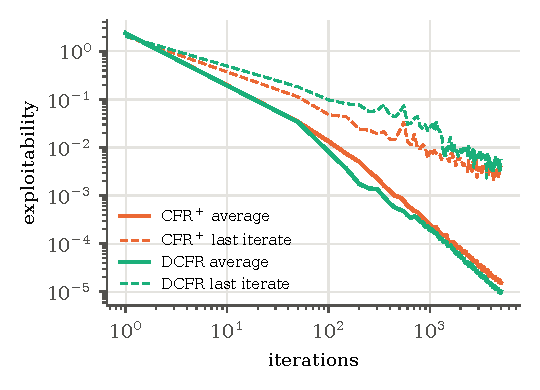
\includegraphics[width=\linewidth]{avg_vs_last.pdf}\\
{\scriptsize Our computation on Leduc. Only the average converges, and each extra digit costs about ten times more iterations.}
\end{columns}
\note{
Make the case without overselling. Precision matters for machines (solving subgames again, evaluation) and for science
(knowing the exact equilibrium, for example the exact bluffing frequencies, or whether a hand mixes at all).\\[3pt]
The analogy for this audience: CFR is like a stationary iterative method. It is fantastic for the first
digits and hopeless for the last ones, and the obvious idea is to switch to a Newton-type method near the solution.\\[3pt]
Numbers for Leduc: CFR$^+$ reaches $\LeducCFRplusLong$ after 50{,}000 iterations and \LeducCFRplusLongTime\ seconds. The curves are on a backup slide.
}
\end{frame}

% =====================================================================================
\begin{frame}{\tagO\ Step 1: write the equilibrium as a variational inequality}
Collect both strategies and both vectors of information-set values in one unknown $z = (x, y, p, q)$. An
equilibrium is a point that satisfies the optimality conditions of both players' linear programs.
\[
\begin{aligned}
 0\le x \ &\perp\ E^\top p - A y \ \ge 0, & Ex &= e,\\
 0\le y \ &\perp\ A^\top x - F^\top q \ \ge 0, & Fy &= f.
\end{aligned}
\]
These conditions have the form $w = Mz + b$ with a matrix that is \textbf{skew-symmetric}.
\[ M = \begin{pmatrix} 0 & -A & E^\top & 0\\ A^\top & 0 & 0 & -F^\top\\ -E & 0 & 0 & 0\\ 0 & F & 0 & 0\end{pmatrix},
   \qquad M + M^\top = 0 . \]
Skew symmetry makes the problem monotone. It also means that the solutions form a polyhedron and
not a single point, so Newton's method cannot be applied directly. CFR gives a starting point for all of $z$ for free.
\note{
This is a mixed linear complementarity problem. The reduced cost $E^\top p - Ay$ of a sequence is its counterfactual
regret scaled by reach, and complementarity says ``play only actions with zero regret''. So CFR and this system talk
about the same quantities: the CFR average strategies are $x$ and $y$, and its best-response values are $p$ and $q$.\\[3pt]
Skewness: the $x$-$y$ block is the zero-sum coupling. The $(x,p)$ and $(y,q)$ blocks are pairs of constraints and multipliers, arranged
with signs so that $M^\top = -M$.\\[3pt]
Non-uniqueness is already visible in Kuhn poker, where the equilibria form a one-parameter family (backup slide).\\[3pt]
If asked what we tried first: Anderson acceleration of the CFR$^+$ map, vector extrapolation of the averages, and Levenberg-Marquardt on the
optimality system. None of them beat DCFR on Leduc. The CFR map is piecewise linear with non-isolated fixed points, and the acceleration theory needs a smooth contraction.
The details are in \texttt{talk-detailed.pdf}.
}
\end{frame}

% =====================================================================================
\begin{frame}{\tagO\ Step 2: the proximal point method makes each problem well posed}
We add a small multiple of the identity. Given $z^k$, the next iterate $z^{k+1}$ solves the same conditions with
\[ w_\rho(z) = (M + \rho I)\,z + b - \rho\, z^{k} . \]
\begin{columns}[T]
\column{0.56\textwidth}
Since $d^\top(M+\rho I)d = \rho\|d\|^2$, the matrix $M+\rho I$ is positive definite and each regularised problem
has exactly one solution.

\medskip
\textbf{Theorem (Rockafellar 1976, Luque 1984).} The iterates converge to a solution of the original problem for every
$\rho>0$. For a polyhedral problem the rate is linear, with a factor that tends to zero with $\rho$.

\medskip
A small $\rho$ gives a fast outer loop and badly conditioned inner problems.
\column{0.41\textwidth}
\begin{block}{Our computation on Leduc with $\rho = 10^{-5}$}
\small The residual after each outer step:\\[2pt]
$3.4\!\times\!10^{-2} \to 4.8\!\times\!10^{-6} \to 3.3\!\times\!10^{-9}$\\ $\to 6.9\!\times\!10^{-12} \to 2.0\!\times\!10^{-14}$\\[3pt]
About three digits for each step.
\end{block}
\end{columns}
\note{
The proximal term fixes the non-uniqueness. Each subproblem has exactly one solution, so Newton's method has a well defined and
nonsingular target. For polyhedral monotone problems the inverse operator is upper Lipschitz (Robinson 1981), which gives linear
convergence of the proximal point method with a factor that tends to zero as $\rho\to0$.\\[3pt]
The trade-off is the whole story of the last part of the talk. A small $\rho$ makes the outer loop fast and the inner problems
nearly as ill posed as the original one, since $\|(M+\rho I)^{-1}\|\le 1/\rho$. There is a backup slide with the rate.
}
\end{frame}

% =====================================================================================
\begin{frame}{\tagO\ Step 3: Newton's method on a piecewise-linear equation}
Each regularised problem can be written as one equation. For every action, either its probability is zero or its
reduced cost is zero, and that is the same as $\min\big(x_i,\ w_\rho(z)_i\big)=0$.

\medskip
A Newton step for this equation guesses which actions are dropped, imposes indifference on all the others, and solves
one linear system. Its matrix has the form $V = D_a + D_b(M+\rho I)$ with nonnegative diagonal matrices $D_a$ and $D_b$.
\begin{block}{Lemma. Every such $V$ with $D_a+D_b$ positive definite is nonsingular.}
\small Suppose $Vd=0$ and put $u = (M+\rho I)d$. Row $i$ reads $(D_a)_{ii}d_i + (D_b)_{ii}u_i = 0$ with nonnegative coefficients
that are not both zero, so $d_i u_i \le 0$. Hence $\rho\|d\|^2 = d^\top u = \sum_i d_i u_i \le 0$, and $d=0$. \hfill$\square$
\end{block}
If the guess of the dropped actions is right, a single step gives the \emph{exact} solution. If it is wrong there is no
global guarantee, so the method needs a good starting guess.
\note{
The min-function turns complementarity into a piecewise-linear equation. Semismooth Newton on it is exactly the
primal-dual active-set method (Hinterm\"uller, Ito and Kunisch 2002). The lemma is the reason
for the proximal term: without $\rho$ we have $d^\top M d = 0$ and the argument fails. Newton matrices of the unregularised problem
are singular at degenerate solutions, which is what we saw with Levenberg-Marquardt.\\[3pt]
The lemma also covers the Fischer-Burmeister reformulation, which has a smooth merit function and a globally convergent damped Newton method.
We tried it first. It worked on Leduc and on a small river with 50 to 70 linear solves, but on the river of the demonstration it
took steps of size $10^{-3}$ for dozens of iterations. That pushed us to the interior-point start on the next slide.
}
\end{frame}

% =====================================================================================
\begin{frame}{\tagO\ Step 4: making it robust and fast}
\begin{columns}[T]
\column{0.55\textwidth}
\textbf{A robust start.} The first regularised problem is the hardest. We solve it with an interior-point method
started at the CFR point. Its solution tells us which actions are dropped, and from there the Newton steps land
exactly on the solution. Every later problem needs only one to three linear solves.

\medskip
\textbf{Fast linear algebra.} After a change of signs in half of the rows, every linear system is symmetric and
\emph{quasi-definite}. By a theorem of Vanderbei, such a matrix has an $LDL^\top$ factorisation for every ordering of
the unknowns, so we can order for sparsity alone and never pivot.
\column{0.42\textwidth}
\begin{block}{One factorisation, in seconds}
\footnotesize
\begin{tabular}{@{}l@{\ \ }c@{\ \ }c@{}}
& small river & our river\\ \midrule
general sparse LU & 0.11 & 25\\
quasi-definite $LDL^\top$ & 0.04 & 7.6
\end{tabular}
\end{block}
\vspace{4pt}
{\small The whole solve from the CFR point to a residual of $10^{-13}$ takes \LeducSolves\ linear solves on Leduc and
\SmallSolves\ on the small river.}
\end{columns}
\note{
The first problem is the hardest because many actions enter or leave the support. The division of labour mirrors what commercial LP solvers do, interior point and then crossover to a vertex, but inside a proximal
loop and with a game-theoretic warm start. We use Mehrotra's predictor-corrector method. In our runs the interior-point phase took 6 to 8 factorisations on Leduc and the small
river, the crossover a few active-set steps, and every later proximal step 1 to 3 steps. We use $\rho=10^{-5}$ throughout.\\[3pt]
Quasi-definite means the block form $\begin{psmallmatrix} P & B\\ B^\top & -N\end{psmallmatrix}$ with $P$ and $N$ positive definite, after grouping $(x,q)$ and $(y,p)$.
Vanderbei's theorem (1995) lets us choose a fill-reducing ordering before seeing the numbers, which is the same reason interior-point
codes like quasi-definite systems. The timings compare SuperLU with QDLDL on one core.\\[3pt]
A caveat: with only $\pm10^{-5}$ on the diagonal, as in the pure active-set systems, static pivoting is too unstable. There we use a
pivoted sparse LU, which is cheap because the active-set system lives on the support only.
}
\end{frame}

% =====================================================================================
\begin{frame}{\tagP\tagO\ Step 5: restrict to the support, solve exactly, then verify}
\begin{columns}[T]
\column{0.54\textwidth}
On larger hands the method so far fails. Many actions are never played and many positions are never
reached, and in those directions the set of equilibria is \emph{flat}. A point with a tiny residual can be far
from a solution, and the Newton step guesses the wrong dropped actions.

\medskip
The cure is to remove those directions. We keep only the actions that DCFR plays with probability above $10^{-3}$ and
solve this smaller problem exactly.

\medskip
Then we check the answer in the full game. If a removed action would have been profitable we put it back and solve again.
\column{0.43\textwidth}
\begin{block}{The complete method}
\small
\begin{enumerate}\setlength\itemsep{2pt}
\item DCFR for a few thousand iterations
\item keep the actions that it uses
\item solve the restricted problem to machine precision
\item compute exact best responses in the full game
\item add back any profitable action and return to 3
\end{enumerate}
\end{block}
{\small Step 4 is a certificate. The final exploitability is measured in the full game and not assumed.}
\end{columns}
\note{
The verification loop is column generation, the same idea as the double-oracle algorithms for games (McMahan, Gordon and Blum 2003,
Bo\v{s}ansk\'y et al.\ 2014). We also keep only the positions that both players can still reach with the kept actions. What is new is the combination with a support predicted by CFR and an exact
second-order solve of the restricted problem.\\[3pt]
Poker helps here. Equilibria are mostly pure, because mixing happens only at indifference. In the exact Leduc equilibrium about half of the
reachable pairs of information set and hand play a single action, and on the small river 71\%. About half of all sequences are outside the
support, and the dense payoff blocks shrink to the hands that actually reach each leaf.\\[3pt]
On our problems Leduc needed 2 rounds, the small river 1, and the river of the demonstration 3, with 16 actions added back in total. The restricted
problem had about 35\% of the unknowns of the full one.
}
\end{frame}

% =====================================================================================
\begin{frame}{\tagO\ Result on the benchmark game, Leduc hold'em}
\begin{columns}[c]
\column{0.6\textwidth}
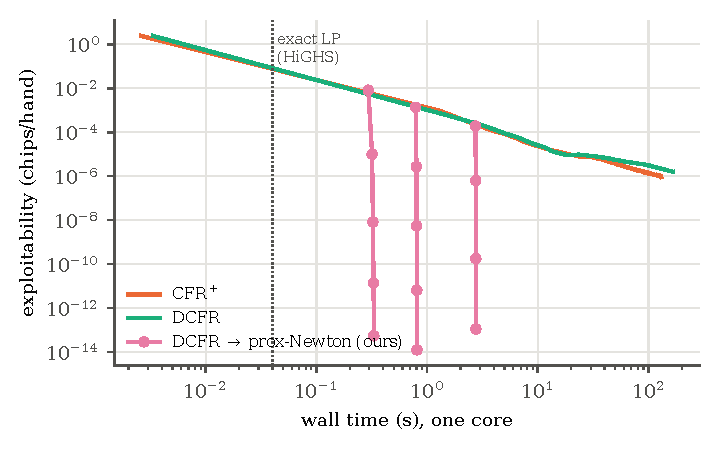
\includegraphics[width=\linewidth]{hybrid_leduc.pdf}
\column{0.38\textwidth}
Each pink curve starts where a short DCFR run stopped and drops straight down to machine precision.

\medskip
From \SuppLeducWarm\ DCFR iterations our method reaches $\SuppLeducExpl$ in \alert{\SuppLeducTime\
seconds}. CFR$^+$ is at $\LeducCFRplusLong$ after \LeducCFRplusLongTime\ seconds.

\medskip
Leduc is tiny and an LP solver needs 0.04 seconds. What matters is the shape of the curves.
\end{columns}
\note{
Each pink curve starts where the DCFR warm start stopped, after 100, 300 or 1000 iterations. The points are verification rounds.
Starting from 100 DCFR iterations is enough and costs one extra round. Starting later only costs DCFR time. The run used \SuppLeducRounds\ rounds and \SuppLeducSolves\ linear solves.\\[3pt]
The value of the game that we obtain, $-0.085606424078\ldots$ chips for the first player, agrees with the LP in all printed digits.\\[3pt]
Be upfront about the LP. Leduc has 964 unknowns and a simplex method finishes in 40 ms. The question is what happens when
the LP does not fit, which is the next slide.
}
\end{frame}

% =====================================================================================
\begin{frame}{\tagO\ Result on the river from the demonstration}
\begin{columns}[T]
\column{0.52\textwidth}
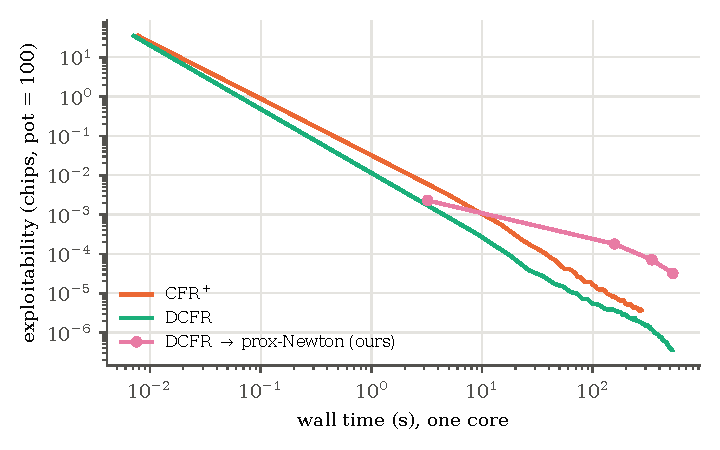
\includegraphics[width=\linewidth]{hybrid_medium.pdf}\\
{\scriptsize 473 against 328 hands and 17{,}626 unknowns. The points are verification rounds.}
\column{0.46\textwidth}
Our method runs DCFR for \SuppMedWarm\ iterations and then needs \SuppMedRounds\ rounds on a problem with \SuppMedFrac\%
of the unknowns. It reaches \alert{$\SuppMedExpl$ chips in \SuppMedTime\ seconds}.

\medskip
At that moment DCFR alone is at $\MedDCFRAtSuppTime$, and after \MedDCFRLongTwoIters\ iterations and \MedDCFRLongTwoTime\
seconds it is at $\MedDCFRLongTwoExpl$.

\medskip
Without the restriction to the support the Newton finish \emph{loses} to DCFR on this hand. The LP solver did not finish in 25
minutes.
\end{columns}
\note{
This is the slide that took the longest to earn. The first version of the method, Newton on the full sequence-form problem, worked
on Leduc and the small river and lost to DCFR here, with $\MedHybExpl$ after \MedHybTime\ seconds. The crossover from the interior point kept landing on a wrong active set,
because the equilibrium set is flat in directions that do not matter, and with
$\rho=10^{-5}$ an error in those directions is amplified by $1/\rho$. A larger $\rho$ made the active-set steps work and the
outer loop crawl. Anderson acceleration of the proximal map helped, to $8\times10^{-7}$ in 8 minutes, and then stalled.\\[3pt]
Restricting to the support predicted by CFR and verifying afterwards removes exactly those directions. \SuppMedAdded\ actions were added back in total.
Starting from 1{,}000 DCFR iterations gives $\SuppMedOneKExpl$ in \SuppMedOneKTime\ seconds.\\[3pt]
On the small river (147 against 139 hands) the method reaches $\SuppSmallExpl$ in \SuppSmallTime\ seconds, DCFR is at $\SmallDCFRExpl$ after \SmallDCFRTime\ seconds, and the LP takes 1.6 seconds. This is on a backup slide.
}
\end{frame}

% =====================================================================================
\begin{frame}{\tagO\ Where it stops winning, and what is open}
\begin{block}{Full ranges: all 1{,}081 hands for both players, 47{,}568 unknowns}
\small The restricted problem still has 43\% of the unknowns and one factorisation takes about 10 seconds. After 80 minutes our
method is at $4.1\times10^{-6}$ chips. DCFR reaches $9.5\times10^{-6}$ in 10 minutes. \textbf{Here CFR wins.}
\end{block}

\medskip
The bottleneck is the linear algebra. Each payoff block is dense, but it is a sorted sign matrix plus a sparse correction,
and a product with it costs $O(n\log n)$. A Newton--Krylov step would then cost only a few CFR iterations, provided we can
find a good preconditioner for systems of the form ``diagonal plus skew''. We think this is the most promising open problem,
and it is a problem in numerical linear algebra.

\medskip
Two further directions are a better prediction of the support from the CFR regrets, which would save verification rounds,
and the use of exact solves inside programs that play in real time.
\note{
The run with full ranges is the honest boundary of the method as implemented. The restriction still removes more than half of the
unknowns, but each factorisation of the remaining system with 20{,}000 unknowns takes about 10 seconds because the payoff blocks between
the hands that remain in play are dense. The first round needed 201 solves and 50 minutes, the second 116, and the second did not
reach machine precision (the proximal loop stalled at a residual of $5\times10^{-7}$).
DCFR does 40{,}000 iterations in 10 minutes.\\[3pt]
The research directions are natural ones for this club. The first is the one I would bet on: the structure that
makes CFR fast (sorting, running sums, card-removal corrections) is exactly the structure that a fast direct or preconditioned iterative
solver for the Newton systems would need. Hierarchical factorisations of the blocks are a candidate.
}
\end{frame}

% =====================================================================================
\begin{frame}{\tagO\ What is new here, and what is not}
The ingredients are classical: the sequence form, the proximal point method, semismooth Newton,
interior point with crossover, quasi-definite factorisations and the CFR family.

\medskip
The closest work is by Yang, Gao, Lin and Kroer (2025), who use a semismooth Newton method for \emph{matrix} games after a
first-order warm start.

\medskip
What we add is a second-order finish that works directly on the sequence form of a poker game. It has four parts:
\begin{itemize}\setlength\itemsep{0pt}
\item the skew formulation with a proximal term, which gives nonsingular Newton matrices by a one-line proof,
\item a warm start for both the strategies and the values taken from CFR,
\item the restriction to the support predicted by CFR, which removes the flat directions,
\item and the verification by exact best responses in the full game.
\end{itemize}
\note{
Be precise about novelty. The general idea of a first-order warm start followed by semismooth Newton for zero-sum games was proposed
for matrix games by Yang, Gao, Lin and Kroer in December 2025 (arXiv 2512.12910). Their Newton system lives on the normal form, they use
Douglas-Rachford splitting and a PRM$^+$ warm start, and they do not treat the structure of extensive-form games.\\[3pt]
To our knowledge no solver based on CFR hands over to a second-order method for the last digits. Early work solved small abstracted games exactly as linear programs (Gilpin and Sandholm 2005). The commercial and research poker solvers that we know of
(PioSolver, GTO+, Libratus, DeepStack) are first-order.
}
\end{frame}

% =====================================================================================
\begin{frame}{Takeaways}
A poker equilibrium is the solution of a structured saddle-point problem, and the sequence form turns it into a linear program
whose size is linear in the game tree.

\medskip
CFR is regret matching at every information set. It never forms the matrix, its proven rate is $T^{-1/2}$, and its modern
variants are much faster in practice, as the race in the browser showed.

\medskip
The output is readable poker: value bets, bluffs, traps and a defence that follows the pot odds.

\medskip
Read as a skew variational inequality, the same problem can be finished by a proximal Newton method. The obstacle is the
flatness of the equilibrium set, and restricting to the support that CFR predicts removes it. On our river this gives
an exploitability of $10^{-12}$ in about two minutes, where DCFR alone is at $10^{-6}$. With full ranges the linear algebra becomes the
bottleneck and CFR wins again.

\medskip
{\small The solver, the interactive page, the benchmarks and these slides are at \texttt{github.com/dwangnumbers/Poker-Solver}.}
\note{
End with the invitation. The open problem on the earlier slide is a natural one for this club: a preconditioner for
shifted skew systems whose off-diagonal blocks are a sorted sign matrix plus a sparse correction.\\[3pt]
If there is time left, go back to the browser and take requests: another board, another range, other bet sizes.
}
\end{frame}

% =====================================================================================
\begin{frame}{Main references}
\footnotesize
\begin{itemize}\setlength\itemsep{1pt}
\item D.~Koller, N.~Megiddo, B.~von Stengel. Efficient computation of equilibria for extensive two-person games. \emph{Games Econ.\ Behav.} 14 (1996).
\item M.~Zinkevich, M.~Johanson, M.~Bowling, C.~Piccione. Regret minimization in games with incomplete information. \emph{NeurIPS} 2007.
\item N.~Brown, T.~Sandholm. Solving imperfect-information games via discounted regret minimization. \emph{AAAI} 2019.
\item R.~T. Rockafellar. Monotone operators and the proximal point algorithm. \emph{SIAM J.\ Control Optim.} 14 (1976).
\item M.~Hinterm\"uller, K.~Ito, K.~Kunisch. The primal-dual active set strategy as a semismooth Newton method. \emph{SIAM J.\ Optim.} 13 (2002).
\item R.~J. Vanderbei. Symmetric quasidefinite matrices. \emph{SIAM J.\ Optim.} 5 (1995).
\item D.~Yang, Y.~Gao, T.~Lin, C.~Kroer. A direct second-order method for solving two-player zero-sum games. arXiv:2512.12910 (2025).
\end{itemize}
The complete list of references is in \texttt{talk-detailed.pdf}.
\end{frame}

% =====================================================================================
\appendix
\begin{frame}{Backup: Kuhn poker, where the equilibrium is not unique}
\begin{columns}[T]
\column{0.55\textwidth}
Kuhn poker uses the three cards \pcard[0.8]{J}{s}\,\pcard[0.8]{Q}{s}\,\pcard[0.8]{K}{s}. Each player puts in one chip and gets one card, and
there is a single bet of one chip.

\medskip
Its equilibria form a one-parameter family. The first player bets the jack as a bluff with any probability
$\alpha$ between 0 and $\tfrac13$, and bets the king with probability $3\alpha$. The value of the game is $-\tfrac1{18}$.

\medskip
The set of equilibria is a polytope and not a point, and any method has to cope with that.
\column{0.42\textwidth}
\begin{block}{Our computation}
\small
The Newton finish returns $\alpha = 0.198$ and bets the king with probability $0.593 = 3\alpha$.\\[2pt]
Value $-0.0555\ldots = -1/18$.\\[2pt]
Exploitability $1.1\times10^{-16}$.
\end{block}
\end{columns}
\note{Kuhn poker is the poker analogue of a two by two test matrix. Jacobians at a solution are
singular, and the proximal term picks one member of the family.}
\end{frame}

\begin{frame}{Backup: the first-order methods on Leduc hold'em}
\begin{columns}[c]
\column{0.58\textwidth}
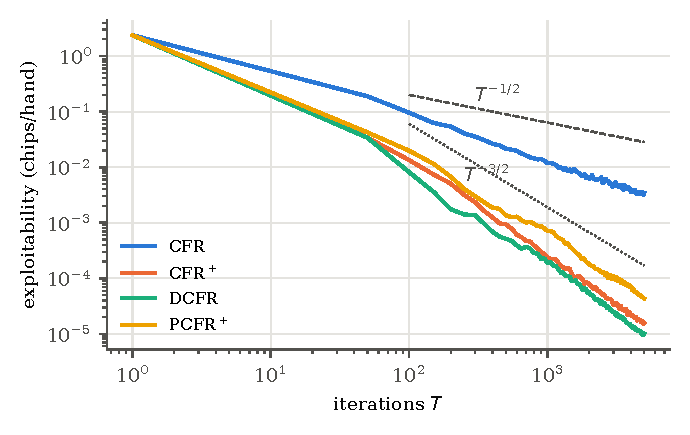
\includegraphics[width=\linewidth]{conv_leduc_iters.pdf}
\column{0.4\textwidth}
The curves show the exploitability of the average strategy for our implementation.

\medskip
After 5{,}000 iterations and \LeducDCFRfiveTime\ seconds DCFR reaches $\LeducDCFRfive$. After 50{,}000 iterations and
\LeducCFRplusLongTime\ seconds CFR$^+$ reaches $\LeducCFRplusLong$ and DCFR $\LeducDCFRLong$.

\medskip
Each extra digit costs about ten times more iterations.
\end{columns}
\note{Exploitability is in chips per hand, and the antes in Leduc are 1 chip.}
\end{frame}

\begin{frame}{Backup: a small river, and every linear solve of one exact solve}
\begin{columns}[c]
\column{0.5\textwidth}
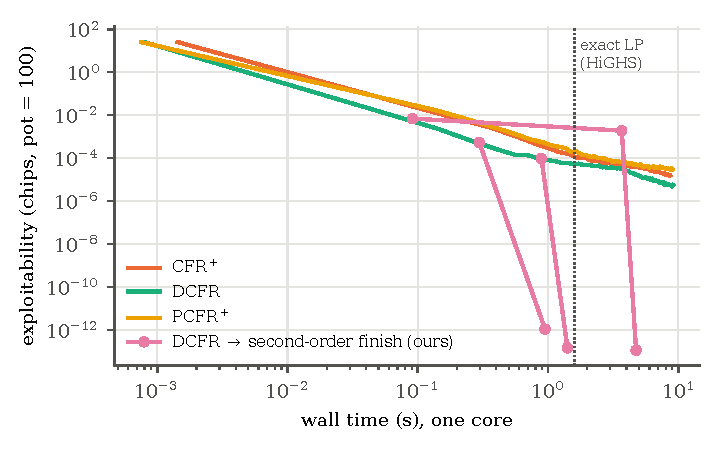
\includegraphics[width=\linewidth]{hybrid_small.pdf}
\column{0.48\textwidth}
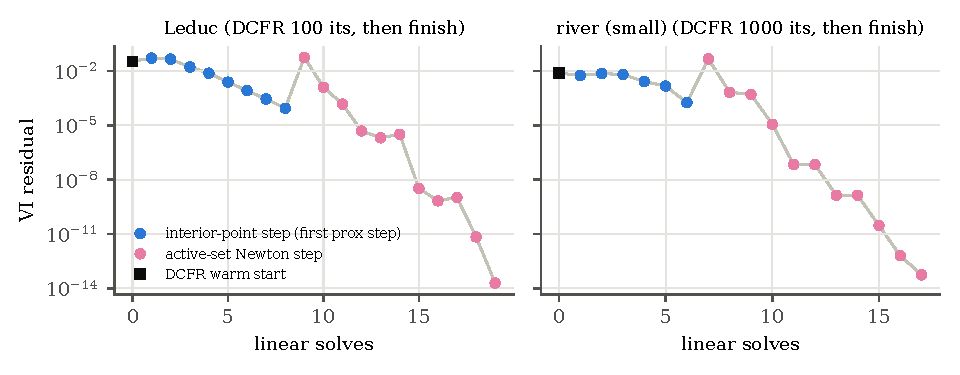
\includegraphics[width=\linewidth]{newton_inner.pdf}
\end{columns}
\medskip
\small On the left is a river with 147 against 139 hands. Our method reaches $\SuppSmallExpl$ chips in \SuppSmallTime\ seconds, DCFR is at
$\SmallDCFRExpl$ after \SmallDCFRTime\ seconds, and the LP takes 1.6 seconds. On the right is the residual after every linear solve. The blue
points are interior-point iterations and the pink points are Newton steps.
\note{The crossover lands on the exact solution of the first regularised
subproblem, whose residual is $\rho\|z^1-z^0\|$, hence the jump. After that each proximal step is solved exactly in one to three steps.}
\end{frame}

\begin{frame}{Backup: the rate of the proximal point method, and why flat equilibria hurt}
The proximal step is the resolvent of a maximal monotone operator $T$, so the iterates move monotonically towards the solution set $Z$.

\medskip
If $T^{-1}$ is upper Lipschitz at $0$ with modulus $a$, which holds for polyhedral problems, then
\[ \operatorname{dist}(z^{k+1}, Z) \ \le\ \frac{a\rho}{\sqrt{1 + a^2\rho^2}}\ \operatorname{dist}(z^k, Z). \]
The modulus $a$ measures how far a point with a small residual can be from $Z$. It is large when the equilibrium set is flat,
that is, when many hands have actions that barely matter.

\medskip
A fast outer loop needs $\rho$ much smaller than $1/a$. But $\|(M+\rho I)^{-1}\|\approx 1/\rho$ then makes the active set of each
subproblem fragile. On Leduc we observe a factor of about $10^{-3}$ for each step at $\rho=10^{-5}$. On the full river of the demonstration no
value of $\rho$ gave both, and the restriction to the support removes the flat directions instead.
\note{Backup for questions about the outer loop. Rockafellar 1976, Luque 1984, Robinson 1981.}
\end{frame}

\end{document}
